\documentclass[twoside]{book}

% Packages required by doxygen
\usepackage{fixltx2e}
\usepackage{calc}
\usepackage{doxygen}
\usepackage[export]{adjustbox} % also loads graphicx
\usepackage{graphicx}
\usepackage[utf8]{inputenc}
\usepackage{makeidx}
\usepackage{multicol}
\usepackage{multirow}
\PassOptionsToPackage{warn}{textcomp}
\usepackage{textcomp}
\usepackage[nointegrals]{wasysym}
\usepackage[table]{xcolor}

% Font selection
\usepackage[T1]{fontenc}
\usepackage[scaled=.90]{helvet}
\usepackage{courier}
\usepackage{amssymb}
\usepackage{sectsty}
\renewcommand{\familydefault}{\sfdefault}
\allsectionsfont{%
  \fontseries{bc}\selectfont%
  \color{darkgray}%
}
\renewcommand{\DoxyLabelFont}{%
  \fontseries{bc}\selectfont%
  \color{darkgray}%
}
\newcommand{\+}{\discretionary{\mbox{\scriptsize$\hookleftarrow$}}{}{}}

% Page & text layout
\usepackage{geometry}
\geometry{%
  a4paper,%
  top=2.5cm,%
  bottom=2.5cm,%
  left=2.5cm,%
  right=2.5cm%
}
\tolerance=750
\hfuzz=15pt
\hbadness=750
\setlength{\emergencystretch}{15pt}
\setlength{\parindent}{0cm}
\setlength{\parskip}{3ex plus 2ex minus 2ex}
\makeatletter
\renewcommand{\paragraph}{%
  \@startsection{paragraph}{4}{0ex}{-1.0ex}{1.0ex}{%
    \normalfont\normalsize\bfseries\SS@parafont%
  }%
}
\renewcommand{\subparagraph}{%
  \@startsection{subparagraph}{5}{0ex}{-1.0ex}{1.0ex}{%
    \normalfont\normalsize\bfseries\SS@subparafont%
  }%
}
\makeatother

% Headers & footers
\usepackage{fancyhdr}
\pagestyle{fancyplain}
\fancyhead[LE]{\fancyplain{}{\bfseries\thepage}}
\fancyhead[CE]{\fancyplain{}{}}
\fancyhead[RE]{\fancyplain{}{\bfseries\leftmark}}
\fancyhead[LO]{\fancyplain{}{\bfseries\rightmark}}
\fancyhead[CO]{\fancyplain{}{}}
\fancyhead[RO]{\fancyplain{}{\bfseries\thepage}}
\fancyfoot[LE]{\fancyplain{}{}}
\fancyfoot[CE]{\fancyplain{}{}}
\fancyfoot[RE]{\fancyplain{}{\bfseries\scriptsize Generated by Doxygen }}
\fancyfoot[LO]{\fancyplain{}{\bfseries\scriptsize Generated by Doxygen }}
\fancyfoot[CO]{\fancyplain{}{}}
\fancyfoot[RO]{\fancyplain{}{}}
\renewcommand{\footrulewidth}{0.4pt}
\renewcommand{\chaptermark}[1]{%
  \markboth{#1}{}%
}
\renewcommand{\sectionmark}[1]{%
  \markright{\thesection\ #1}%
}

% Indices & bibliography
\usepackage{natbib}
\usepackage[titles]{tocloft}
\setcounter{tocdepth}{3}
\setcounter{secnumdepth}{5}
\makeindex

% Hyperlinks (required, but should be loaded last)
\usepackage{ifpdf}
\ifpdf
  \usepackage[pdftex,pagebackref=true]{hyperref}
\else
  \usepackage[ps2pdf,pagebackref=true]{hyperref}
\fi
\hypersetup{%
  colorlinks=true,%
  linkcolor=blue,%
  citecolor=blue,%
  unicode%
}

% Custom commands
\newcommand{\clearemptydoublepage}{%
  \newpage{\pagestyle{empty}\cleardoublepage}%
}

\usepackage{caption}
\captionsetup{labelsep=space,justification=centering,font={bf},singlelinecheck=off,skip=4pt,position=top}

%===== C O N T E N T S =====

\begin{document}

% Titlepage & ToC
\hypersetup{pageanchor=false,
             bookmarksnumbered=true,
             pdfencoding=unicode
            }
\pagenumbering{alph}
\begin{titlepage}
\vspace*{7cm}
\begin{center}%
{\Large I\+T\+Company\+Cpp \\[1ex]\large I\+T\+Company\+Cpp }\\
\vspace*{1cm}
{\large Generated by Doxygen 1.8.13}\\
\end{center}
\end{titlepage}
\clearemptydoublepage
\pagenumbering{roman}
\tableofcontents
\clearemptydoublepage
\pagenumbering{arabic}
\hypersetup{pageanchor=true}

%--- Begin generated contents ---
\chapter{Class Index}
\section{Class List}
Here are the classes, structs, unions and interfaces with brief descriptions\+:\begin{DoxyCompactList}
\item\contentsline{section}{\hyperlink{class_documents}{Documents} \\*\hyperlink{class_documents}{Documents} class }{\pageref{class_documents}}{}
\item\contentsline{section}{\hyperlink{class_employee}{Employee} \\*\hyperlink{class_employee}{Employee} class }{\pageref{class_employee}}{}
\item\contentsline{section}{\hyperlink{class_h_r}{HR} \\*\hyperlink{class_h_r}{HR} class }{\pageref{class_h_r}}{}
\item\contentsline{section}{\hyperlink{class_i_t___company}{I\+T\+\_\+\+Company} \\*I\+T\+Company class }{\pageref{class_i_t___company}}{}
\item\contentsline{section}{\hyperlink{class_personal_card}{Personal\+Card} \\*\hyperlink{class_personal_card}{Personal\+Card} class }{\pageref{class_personal_card}}{}
\end{DoxyCompactList}

\chapter{File Index}
\section{File List}
Here is a list of all files with brief descriptions\+:\begin{DoxyCompactList}
\item\contentsline{section}{C\+:/\+Workspace/\+I\+T\+Company\+Cpp/\+I\+T\+Company/\+I\+T\+Company/\hyperlink{_documents_8cpp}{Documents.\+cpp} }{\pageref{_documents_8cpp}}{}
\item\contentsline{section}{C\+:/\+Workspace/\+I\+T\+Company\+Cpp/\+I\+T\+Company/\+I\+T\+Company/\hyperlink{_documents_8h}{Documents.\+h} }{\pageref{_documents_8h}}{}
\item\contentsline{section}{C\+:/\+Workspace/\+I\+T\+Company\+Cpp/\+I\+T\+Company/\+I\+T\+Company/\hyperlink{_employee_8cpp}{Employee.\+cpp} }{\pageref{_employee_8cpp}}{}
\item\contentsline{section}{C\+:/\+Workspace/\+I\+T\+Company\+Cpp/\+I\+T\+Company/\+I\+T\+Company/\hyperlink{_employee_8h}{Employee.\+h} }{\pageref{_employee_8h}}{}
\item\contentsline{section}{C\+:/\+Workspace/\+I\+T\+Company\+Cpp/\+I\+T\+Company/\+I\+T\+Company/\hyperlink{_h_r_8cpp}{H\+R.\+cpp} }{\pageref{_h_r_8cpp}}{}
\item\contentsline{section}{C\+:/\+Workspace/\+I\+T\+Company\+Cpp/\+I\+T\+Company/\+I\+T\+Company/\hyperlink{_h_r_8h}{H\+R.\+h} }{\pageref{_h_r_8h}}{}
\item\contentsline{section}{C\+:/\+Workspace/\+I\+T\+Company\+Cpp/\+I\+T\+Company/\+I\+T\+Company/\hyperlink{_i_t___company_8cpp}{I\+T\+\_\+\+Company.\+cpp} }{\pageref{_i_t___company_8cpp}}{}
\item\contentsline{section}{C\+:/\+Workspace/\+I\+T\+Company\+Cpp/\+I\+T\+Company/\+I\+T\+Company/\hyperlink{_i_t___company_8h}{I\+T\+\_\+\+Company.\+h} }{\pageref{_i_t___company_8h}}{}
\item\contentsline{section}{C\+:/\+Workspace/\+I\+T\+Company\+Cpp/\+I\+T\+Company/\+I\+T\+Company/\hyperlink{_main_8cpp}{Main.\+cpp} }{\pageref{_main_8cpp}}{}
\item\contentsline{section}{C\+:/\+Workspace/\+I\+T\+Company\+Cpp/\+I\+T\+Company/\+I\+T\+Company/\hyperlink{_personal_card_8cpp}{Personal\+Card.\+cpp} }{\pageref{_personal_card_8cpp}}{}
\item\contentsline{section}{C\+:/\+Workspace/\+I\+T\+Company\+Cpp/\+I\+T\+Company/\+I\+T\+Company/\hyperlink{_personal_card_8h}{Personal\+Card.\+h} }{\pageref{_personal_card_8h}}{}
\end{DoxyCompactList}

\chapter{Class Documentation}
\hypertarget{class_documents}{}\section{Documents Class Reference}
\label{class_documents}\index{Documents@{Documents}}


\hyperlink{class_documents}{Documents} class.  




{\ttfamily \#include $<$Documents.\+h$>$}

\subsection*{Public Member Functions}
\begin{DoxyCompactItemize}
\item 
\mbox{\Hypertarget{class_documents_a52daba61782250a38f4964910a961793}\label{class_documents_a52daba61782250a38f4964910a961793}} 
\hyperlink{class_documents_a52daba61782250a38f4964910a961793}{Documents} ()
\begin{DoxyCompactList}\small\item\em Default constructor. \end{DoxyCompactList}\item 
\mbox{\Hypertarget{class_documents_a67e92e6e30aeff0300ac69e55bd2aab0}\label{class_documents_a67e92e6e30aeff0300ac69e55bd2aab0}} 
\hyperlink{class_documents_a67e92e6e30aeff0300ac69e55bd2aab0}{$\sim$\+Documents} ()
\begin{DoxyCompactList}\small\item\em Destructor. \end{DoxyCompactList}\item 
\mbox{\Hypertarget{class_documents_a524740a8fbe3933562d63c9999c0cb53}\label{class_documents_a524740a8fbe3933562d63c9999c0cb53}} 
std\+::string \hyperlink{class_documents_a524740a8fbe3933562d63c9999c0cb53}{Create} ()
\begin{DoxyCompactList}\small\item\em Creation method. \end{DoxyCompactList}\item 
\mbox{\Hypertarget{class_documents_aa101f46efd37c76443f90822407bcaa3}\label{class_documents_aa101f46efd37c76443f90822407bcaa3}} 
void \hyperlink{class_documents_aa101f46efd37c76443f90822407bcaa3}{Set\+Order\+To\+Accept} (string v\+\_\+\+Order\+To\+Accept)
\begin{DoxyCompactList}\small\item\em Setter Order to accept. \end{DoxyCompactList}\item 
\mbox{\Hypertarget{class_documents_ae91e6dba2623a69fafd9b886093087d0}\label{class_documents_ae91e6dba2623a69fafd9b886093087d0}} 
void \hyperlink{class_documents_ae91e6dba2623a69fafd9b886093087d0}{Set\+Order\+To\+Dismission} (string v\+\_\+\+Order\+To\+Dismission)
\begin{DoxyCompactList}\small\item\em Setter Order to dismiss. \end{DoxyCompactList}\item 
\mbox{\Hypertarget{class_documents_a484f3e195b0ab7383ef09278cd95907f}\label{class_documents_a484f3e195b0ab7383ef09278cd95907f}} 
void \hyperlink{class_documents_a484f3e195b0ab7383ef09278cd95907f}{Set\+Order\+To\+Give\+Vacation} (string v\+\_\+\+Order\+To\+Give\+Vacation)
\begin{DoxyCompactList}\small\item\em Setter Order give vacation. \end{DoxyCompactList}\item 
\mbox{\Hypertarget{class_documents_a49f95590b3808cdada6632f702213bfa}\label{class_documents_a49f95590b3808cdada6632f702213bfa}} 
void \hyperlink{class_documents_a49f95590b3808cdada6632f702213bfa}{Set\+Employment\+History\+Book} (string v\+\_\+\+Employment\+History\+Book)
\begin{DoxyCompactList}\small\item\em Setter employment history book. \end{DoxyCompactList}\item 
\mbox{\Hypertarget{class_documents_aac5573ba9b558530c669eccf178e3879}\label{class_documents_aac5573ba9b558530c669eccf178e3879}} 
string {\bfseries Get\+Order\+To\+Accept} ()
\item 
\mbox{\Hypertarget{class_documents_a47d56daa1f7434c712707bec1c827ea2}\label{class_documents_a47d56daa1f7434c712707bec1c827ea2}} 
string {\bfseries Get\+Order\+To\+Dismission} ()
\item 
\mbox{\Hypertarget{class_documents_ab13dc4fd233d75d6be5a39142ad99b13}\label{class_documents_ab13dc4fd233d75d6be5a39142ad99b13}} 
string {\bfseries Get\+Order\+To\+Give\+Vacation} ()
\item 
\mbox{\Hypertarget{class_documents_a44b0e6798731de568258ff317c6700da}\label{class_documents_a44b0e6798731de568258ff317c6700da}} 
string {\bfseries Get\+Employment\+History\+Book} ()
\item 
\mbox{\Hypertarget{class_documents_a97d69eea71291c43d6c344c4efeb8fc6}\label{class_documents_a97d69eea71291c43d6c344c4efeb8fc6}} 
bool {\bfseries Check\+Order\+To\+Dismiss} (string order\+To\+Dismiss)
\end{DoxyCompactItemize}
\subsection*{Public Attributes}
\begin{DoxyCompactItemize}
\item 
\mbox{\Hypertarget{class_documents_a28e850b0505533696603105c57450770}\label{class_documents_a28e850b0505533696603105c57450770}} 
std\+::string \hyperlink{class_documents_a28e850b0505533696603105c57450770}{Employment\+Contract}
\begin{DoxyCompactList}\small\item\em Employment contract. \end{DoxyCompactList}\end{DoxyCompactItemize}
\subsection*{Private Member Functions}
\begin{DoxyCompactItemize}
\item 
\mbox{\Hypertarget{class_documents_a7f06bda36f9fe48a22a8c511aa1e2d06}\label{class_documents_a7f06bda36f9fe48a22a8c511aa1e2d06}} 
string \hyperlink{class_documents_a7f06bda36f9fe48a22a8c511aa1e2d06}{Docs\+\_\+\+Utility} ()
\begin{DoxyCompactList}\small\item\em Utility function. \end{DoxyCompactList}\end{DoxyCompactItemize}
\subsection*{Private Attributes}
\begin{DoxyCompactItemize}
\item 
\mbox{\Hypertarget{class_documents_aeee4dc66716ab38efeae09702bc8feed}\label{class_documents_aeee4dc66716ab38efeae09702bc8feed}} 
string \hyperlink{class_documents_aeee4dc66716ab38efeae09702bc8feed}{Order\+To\+Accept}
\begin{DoxyCompactList}\small\item\em Order to accept. \end{DoxyCompactList}\item 
\mbox{\Hypertarget{class_documents_a6d875e6e5ac48c55f9d9121ef302ac50}\label{class_documents_a6d875e6e5ac48c55f9d9121ef302ac50}} 
string \hyperlink{class_documents_a6d875e6e5ac48c55f9d9121ef302ac50}{Order\+To\+Dismission}
\begin{DoxyCompactList}\small\item\em Order to dismiss. \end{DoxyCompactList}\item 
\mbox{\Hypertarget{class_documents_ad55168aa0283ea51d965e732d52bee5a}\label{class_documents_ad55168aa0283ea51d965e732d52bee5a}} 
string \hyperlink{class_documents_ad55168aa0283ea51d965e732d52bee5a}{Order\+To\+Give\+Vacation}
\begin{DoxyCompactList}\small\item\em Vacation order. \end{DoxyCompactList}\item 
\mbox{\Hypertarget{class_documents_ab78a87bb29b653f803e657e6406905b4}\label{class_documents_ab78a87bb29b653f803e657e6406905b4}} 
string \hyperlink{class_documents_ab78a87bb29b653f803e657e6406905b4}{Employment\+History\+Book}
\begin{DoxyCompactList}\small\item\em Employment history. \end{DoxyCompactList}\end{DoxyCompactItemize}


\subsection{Detailed Description}
\hyperlink{class_documents}{Documents} class. 

Definition at line 10 of file Documents.\+h.



The documentation for this class was generated from the following files\+:\begin{DoxyCompactItemize}
\item 
C\+:/\+Workspace/\+I\+T\+Company\+Cpp/\+I\+T\+Company/\+I\+T\+Company/Documents.\+h\item 
C\+:/\+Workspace/\+I\+T\+Company\+Cpp/\+I\+T\+Company/\+I\+T\+Company/Documents.\+cpp\end{DoxyCompactItemize}

\hypertarget{class_employee}{}\section{Employee Class Reference}
\label{class_employee}\index{Employee@{Employee}}


\hyperlink{class_employee}{Employee} class.  




{\ttfamily \#include $<$Employee.\+h$>$}



Collaboration diagram for Employee\+:\nopagebreak
\begin{figure}[H]
\begin{center}
\leavevmode
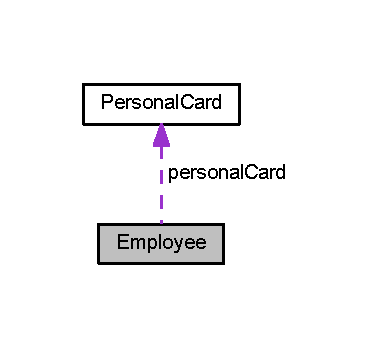
\includegraphics[width=179pt]{class_employee__coll__graph}
\end{center}
\end{figure}
\subsection*{Public Member Functions}
\begin{DoxyCompactItemize}
\item 
\hyperlink{class_employee_a003c7bd08c40924e381eb0750cbb906f}{Employee} ()
\begin{DoxyCompactList}\small\item\em Default constructor. \end{DoxyCompactList}\item 
\hyperlink{class_employee_abed56e9c007fff2bfe27ca87251baaf2}{$\sim$\+Employee} ()
\begin{DoxyCompactList}\small\item\em Destructor. \end{DoxyCompactList}\item 
void \hyperlink{class_employee_a0bec05aa09e9a7a12e3c3de49c43c158}{Dismiss} (void)
\begin{DoxyCompactList}\small\item\em O\+Rder to dismiss. \end{DoxyCompactList}\item 
string \hyperlink{class_employee_ae210ea3433b4596f9d3ff5dee4c63bc2}{Get\+New\+Position} (void)
\begin{DoxyCompactList}\small\item\em Returns new position. \end{DoxyCompactList}\item 
int \hyperlink{class_employee_a8644c276b8a3cdb8bb62a71a492e574d}{Go\+On\+Training\+Courses} (void)
\begin{DoxyCompactList}\small\item\em Sends to training course. \end{DoxyCompactList}\item 
string \hyperlink{class_employee_a37e77828f9f559a27951e3113b3fb520}{Give\+Resume} (void)
\begin{DoxyCompactList}\small\item\em Returns CV. \end{DoxyCompactList}\item 
string \hyperlink{class_employee_ad7a5d34564702bc8b880db1714c75413}{Accept\+Employment\+Contract} (void)
\item 
void \hyperlink{class_employee_a62cc0f19d969528e061ad178a1b109ac}{Set\+Date\+Of\+Acception} (string v\+\_\+\+Date\+Of\+Acception)
\item 
void \hyperlink{class_employee_a7eebc60f8cfd43fe07fae6196a317b0c}{Set\+Cause\+Of\+Acception} (string v\+\_\+\+Cause\+Of\+Acception)
\item 
void \hyperlink{class_employee_ae0a2d5a5ec36af567bc7e434d18de422}{Set\+Number\+Of\+Acceptional\+Order} (int v\+\_\+\+Number\+Of\+Acceptional\+Order)
\item 
void \hyperlink{class_employee_acbb98daeb702b22d616c8b7064784210}{Set\+Date\+Of\+Dismiss} (string v\+\_\+\+Date\+Of\+Dismiss)
\item 
void \hyperlink{class_employee_ac129a41d2cb756360ad056bf39c25464}{Set\+Cause\+Of\+Dismission} (string v\+\_\+\+Cause\+Of\+Dismission)
\item 
void \hyperlink{class_employee_abcf46d071f43b17f0a83b00a327822b9}{Set\+Number\+Of\+Dismissal\+Order} (int v\+\_\+\+Number\+Of\+Dismissal\+Order)
\item 
void \hyperlink{class_employee_a3ffb3c8c2dc4817f88801be832eb8caa}{Set\+Date\+Of\+Returning\+Money} (string v\+\_\+\+Date\+Of\+Returning\+Money)
\item 
string \hyperlink{class_employee_ad8df9b482bc23365e06357005524c5fd}{Get\+Date\+Of\+Acception} ()
\item 
string \hyperlink{class_employee_a462e85cd69817614a7c9e030fb806f29}{Get\+Cause\+Of\+Acception} ()
\item 
int \hyperlink{class_employee_a8ad22e912e2e4e336416df20480ceb54}{Get\+Number\+Of\+Acceptional\+Order} ()
\item 
string \hyperlink{class_employee_a9bf98793dad6f452b3b99b353a4a6635}{Get\+Date\+Of\+Dismiss} ()
\item 
string \hyperlink{class_employee_aa7e35077b13efe6cbc362dc7b561b010}{Get\+Cause\+Of\+Dismission} ()
\item 
int \hyperlink{class_employee_a521952ca263ba6ad783c634631070076}{Get\+Number\+Of\+Dismissal\+Order} ()
\item 
string \hyperlink{class_employee_a7782178746f3640942450a0f7271ef60}{Get\+Date\+Of\+Returning\+Money} ()
\item 
bool \hyperlink{class_employee_a48638241e63b03873954369b285d1cd9}{Check\+Number\+Of\+Acceptional\+Order} (int number\+Of\+Acceptional\+Order)
\item 
bool \hyperlink{class_employee_ac7bf1d7191d60ada37e85f8d311a254d}{Check\+Number\+Of\+Dismissal\+Order} (int number\+Of\+Dismissal\+Order)
\end{DoxyCompactItemize}
\subsection*{Private Member Functions}
\begin{DoxyCompactItemize}
\item 
void \hyperlink{class_employee_a6d9c2cbf05d3137a24c322b1525fffa2}{Employee\+\_\+\+Utility\+\_\+\+Dismiss} ()
\item 
void \hyperlink{class_employee_a534f83eb6f2f106f72d802fcae00eb14}{Employee\+\_\+\+Utility\+\_\+\+Accept} ()
\end{DoxyCompactItemize}
\subsection*{Private Attributes}
\begin{DoxyCompactItemize}
\item 
string \hyperlink{class_employee_a4b6f93cebcc5e3bb343f89d65467c4d2}{Date\+Of\+Acception}
\item 
string \hyperlink{class_employee_ae218a1ea5ff298c3501afa8e815da9d7}{Cause\+Of\+Acception}
\item 
int \hyperlink{class_employee_aafefc3b0042fe3cf88dff13a6458e5de}{Number\+Of\+Acceptional\+Order}
\item 
string \hyperlink{class_employee_a1402b4d32163d3fca601082052d2ff80}{Date\+Of\+Dismiss}
\item 
string \hyperlink{class_employee_a80bd5a84291a0369521af1dcfecca970}{Cause\+Of\+Dismission}
\item 
int \hyperlink{class_employee_a0dc06d409299d253f240ceb01d1a3faf}{Number\+Of\+Dismissal\+Order}
\item 
string \hyperlink{class_employee_a05233437fad4de82175600c04552f0ca}{Date\+Of\+Returning\+Money}
\item 
\hyperlink{class_personal_card}{Personal\+Card} \hyperlink{class_employee_a3a0668e43e943ba0ac0ad0470de8599a}{personal\+Card}
\end{DoxyCompactItemize}


\subsection{Detailed Description}
\hyperlink{class_employee}{Employee} class. 

Definition at line 13 of file Employee.\+h.



\subsection{Constructor \& Destructor Documentation}
\mbox{\Hypertarget{class_employee_a003c7bd08c40924e381eb0750cbb906f}\label{class_employee_a003c7bd08c40924e381eb0750cbb906f}} 
\index{Employee@{Employee}!Employee@{Employee}}
\index{Employee@{Employee}!Employee@{Employee}}
\subsubsection{\texorpdfstring{Employee()}{Employee()}}
{\footnotesize\ttfamily Employee\+::\+Employee (\begin{DoxyParamCaption}{ }\end{DoxyParamCaption})}



Default constructor. 



Definition at line 4 of file Employee.\+cpp.

\mbox{\Hypertarget{class_employee_abed56e9c007fff2bfe27ca87251baaf2}\label{class_employee_abed56e9c007fff2bfe27ca87251baaf2}} 
\index{Employee@{Employee}!````~Employee@{$\sim$\+Employee}}
\index{````~Employee@{$\sim$\+Employee}!Employee@{Employee}}
\subsubsection{\texorpdfstring{$\sim$\+Employee()}{~Employee()}}
{\footnotesize\ttfamily Employee\+::$\sim$\+Employee (\begin{DoxyParamCaption}{ }\end{DoxyParamCaption})}



Destructor. 



Definition at line 7 of file Employee.\+cpp.



\subsection{Member Function Documentation}
\mbox{\Hypertarget{class_employee_ad7a5d34564702bc8b880db1714c75413}\label{class_employee_ad7a5d34564702bc8b880db1714c75413}} 
\index{Employee@{Employee}!Accept\+Employment\+Contract@{Accept\+Employment\+Contract}}
\index{Accept\+Employment\+Contract@{Accept\+Employment\+Contract}!Employee@{Employee}}
\subsubsection{\texorpdfstring{Accept\+Employment\+Contract()}{AcceptEmploymentContract()}}
{\footnotesize\ttfamily std\+::string Employee\+::\+Accept\+Employment\+Contract (\begin{DoxyParamCaption}\item[{void}]{ }\end{DoxyParamCaption})}



Definition at line 88 of file Employee.\+cpp.

Here is the call graph for this function\+:
\nopagebreak
\begin{figure}[H]
\begin{center}
\leavevmode
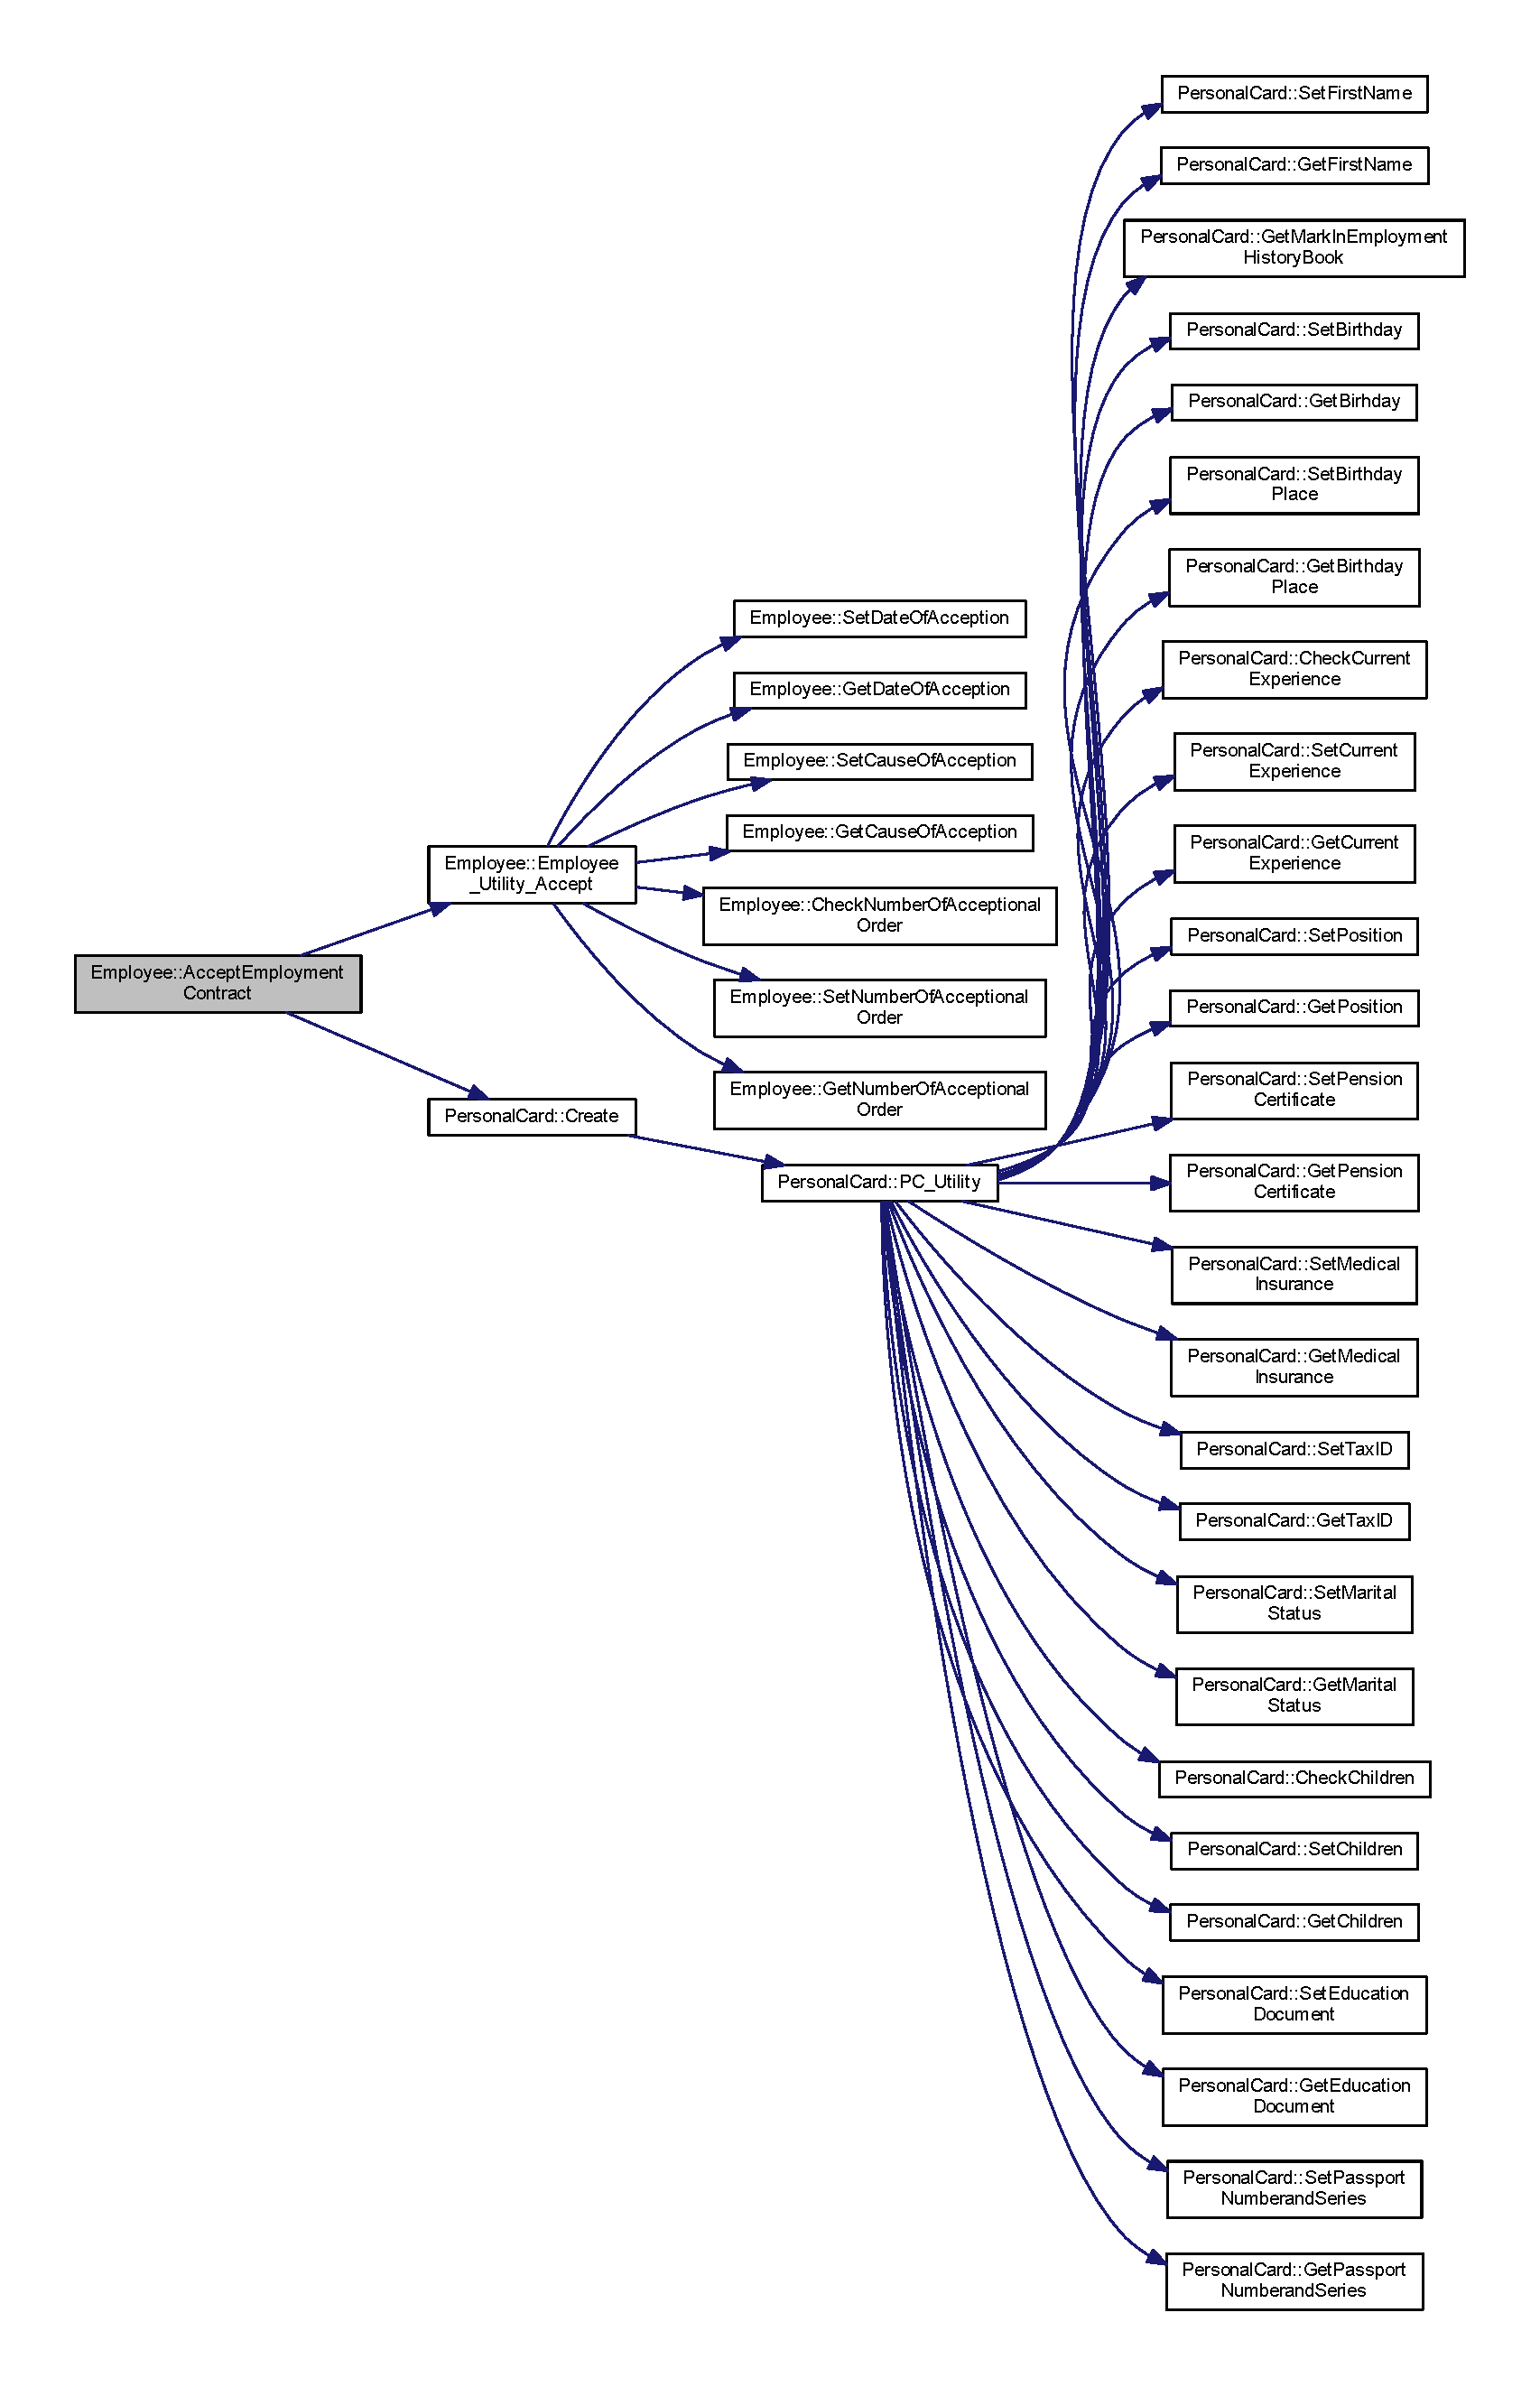
\includegraphics[width=350pt]{class_employee_ad7a5d34564702bc8b880db1714c75413_cgraph}
\end{center}
\end{figure}
\mbox{\Hypertarget{class_employee_a48638241e63b03873954369b285d1cd9}\label{class_employee_a48638241e63b03873954369b285d1cd9}} 
\index{Employee@{Employee}!Check\+Number\+Of\+Acceptional\+Order@{Check\+Number\+Of\+Acceptional\+Order}}
\index{Check\+Number\+Of\+Acceptional\+Order@{Check\+Number\+Of\+Acceptional\+Order}!Employee@{Employee}}
\subsubsection{\texorpdfstring{Check\+Number\+Of\+Acceptional\+Order()}{CheckNumberOfAcceptionalOrder()}}
{\footnotesize\ttfamily bool Employee\+::\+Check\+Number\+Of\+Acceptional\+Order (\begin{DoxyParamCaption}\item[{int}]{number\+Of\+Acceptional\+Order }\end{DoxyParamCaption})}



Definition at line 153 of file Employee.\+cpp.

Here is the caller graph for this function\+:
\nopagebreak
\begin{figure}[H]
\begin{center}
\leavevmode
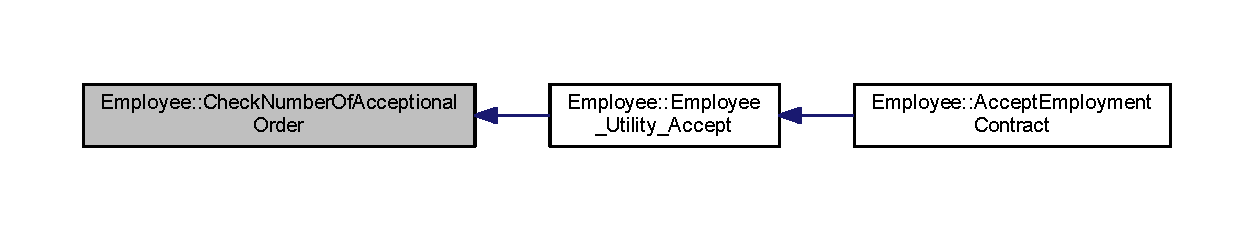
\includegraphics[width=350pt]{class_employee_a48638241e63b03873954369b285d1cd9_icgraph}
\end{center}
\end{figure}
\mbox{\Hypertarget{class_employee_ac7bf1d7191d60ada37e85f8d311a254d}\label{class_employee_ac7bf1d7191d60ada37e85f8d311a254d}} 
\index{Employee@{Employee}!Check\+Number\+Of\+Dismissal\+Order@{Check\+Number\+Of\+Dismissal\+Order}}
\index{Check\+Number\+Of\+Dismissal\+Order@{Check\+Number\+Of\+Dismissal\+Order}!Employee@{Employee}}
\subsubsection{\texorpdfstring{Check\+Number\+Of\+Dismissal\+Order()}{CheckNumberOfDismissalOrder()}}
{\footnotesize\ttfamily bool Employee\+::\+Check\+Number\+Of\+Dismissal\+Order (\begin{DoxyParamCaption}\item[{int}]{number\+Of\+Dismissal\+Order }\end{DoxyParamCaption})}



Definition at line 159 of file Employee.\+cpp.

Here is the caller graph for this function\+:
\nopagebreak
\begin{figure}[H]
\begin{center}
\leavevmode
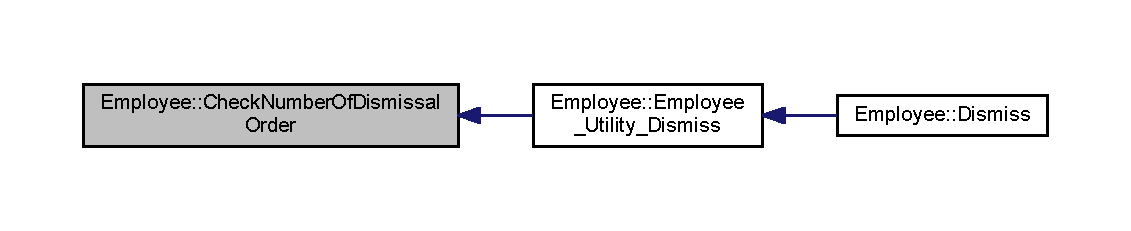
\includegraphics[width=350pt]{class_employee_ac7bf1d7191d60ada37e85f8d311a254d_icgraph}
\end{center}
\end{figure}
\mbox{\Hypertarget{class_employee_a0bec05aa09e9a7a12e3c3de49c43c158}\label{class_employee_a0bec05aa09e9a7a12e3c3de49c43c158}} 
\index{Employee@{Employee}!Dismiss@{Dismiss}}
\index{Dismiss@{Dismiss}!Employee@{Employee}}
\subsubsection{\texorpdfstring{Dismiss()}{Dismiss()}}
{\footnotesize\ttfamily void Employee\+::\+Dismiss (\begin{DoxyParamCaption}\item[{void}]{ }\end{DoxyParamCaption})}



O\+Rder to dismiss. 



Definition at line 72 of file Employee.\+cpp.

Here is the call graph for this function\+:
\nopagebreak
\begin{figure}[H]
\begin{center}
\leavevmode
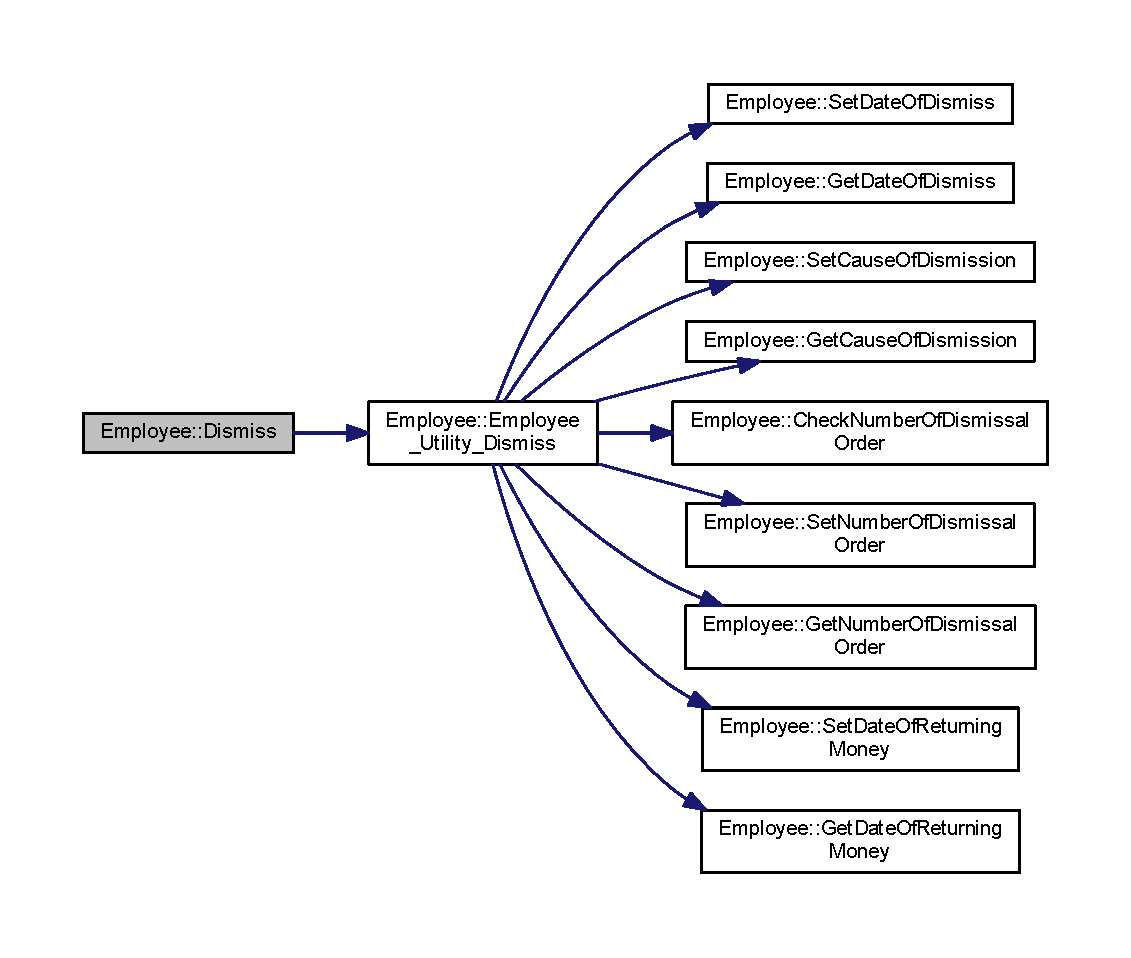
\includegraphics[width=350pt]{class_employee_a0bec05aa09e9a7a12e3c3de49c43c158_cgraph}
\end{center}
\end{figure}
\mbox{\Hypertarget{class_employee_a534f83eb6f2f106f72d802fcae00eb14}\label{class_employee_a534f83eb6f2f106f72d802fcae00eb14}} 
\index{Employee@{Employee}!Employee\+\_\+\+Utility\+\_\+\+Accept@{Employee\+\_\+\+Utility\+\_\+\+Accept}}
\index{Employee\+\_\+\+Utility\+\_\+\+Accept@{Employee\+\_\+\+Utility\+\_\+\+Accept}!Employee@{Employee}}
\subsubsection{\texorpdfstring{Employee\+\_\+\+Utility\+\_\+\+Accept()}{Employee\_Utility\_Accept()}}
{\footnotesize\ttfamily void Employee\+::\+Employee\+\_\+\+Utility\+\_\+\+Accept (\begin{DoxyParamCaption}{ }\end{DoxyParamCaption})\hspace{0.3cm}{\ttfamily [private]}}



Definition at line 10 of file Employee.\+cpp.

Here is the call graph for this function\+:
\nopagebreak
\begin{figure}[H]
\begin{center}
\leavevmode
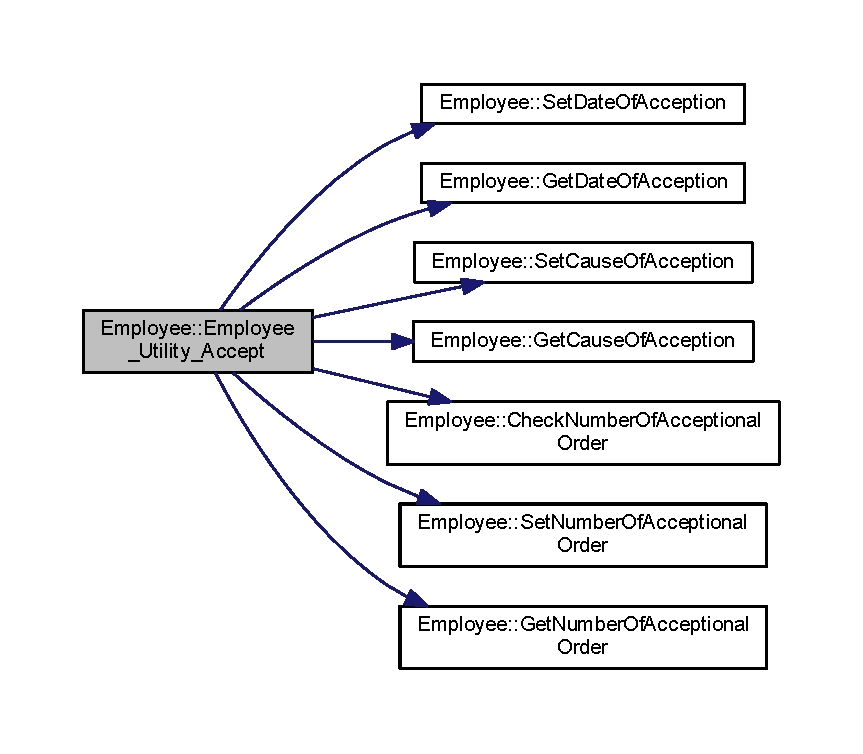
\includegraphics[width=350pt]{class_employee_a534f83eb6f2f106f72d802fcae00eb14_cgraph}
\end{center}
\end{figure}
Here is the caller graph for this function\+:
\nopagebreak
\begin{figure}[H]
\begin{center}
\leavevmode
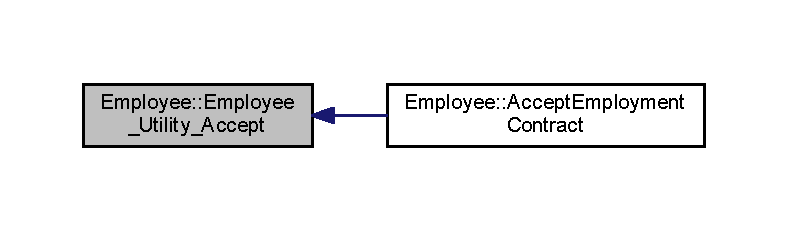
\includegraphics[width=350pt]{class_employee_a534f83eb6f2f106f72d802fcae00eb14_icgraph}
\end{center}
\end{figure}
\mbox{\Hypertarget{class_employee_a6d9c2cbf05d3137a24c322b1525fffa2}\label{class_employee_a6d9c2cbf05d3137a24c322b1525fffa2}} 
\index{Employee@{Employee}!Employee\+\_\+\+Utility\+\_\+\+Dismiss@{Employee\+\_\+\+Utility\+\_\+\+Dismiss}}
\index{Employee\+\_\+\+Utility\+\_\+\+Dismiss@{Employee\+\_\+\+Utility\+\_\+\+Dismiss}!Employee@{Employee}}
\subsubsection{\texorpdfstring{Employee\+\_\+\+Utility\+\_\+\+Dismiss()}{Employee\_Utility\_Dismiss()}}
{\footnotesize\ttfamily void Employee\+::\+Employee\+\_\+\+Utility\+\_\+\+Dismiss (\begin{DoxyParamCaption}{ }\end{DoxyParamCaption})\hspace{0.3cm}{\ttfamily [private]}}



Definition at line 38 of file Employee.\+cpp.

Here is the call graph for this function\+:
\nopagebreak
\begin{figure}[H]
\begin{center}
\leavevmode
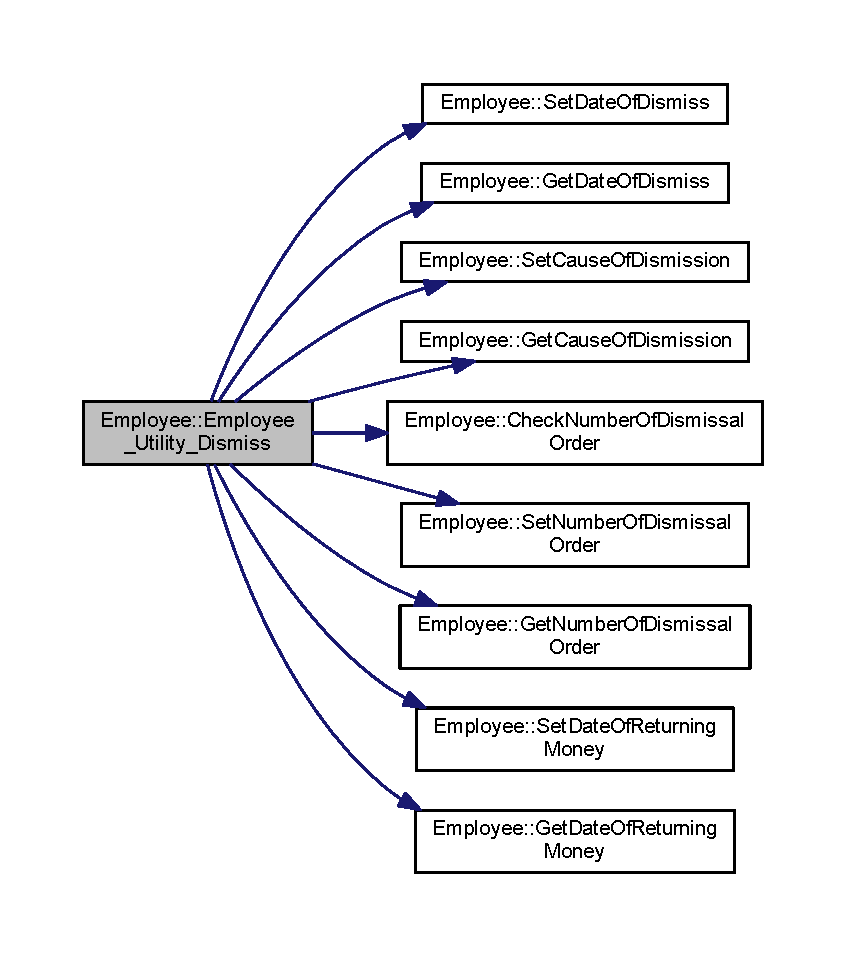
\includegraphics[width=350pt]{class_employee_a6d9c2cbf05d3137a24c322b1525fffa2_cgraph}
\end{center}
\end{figure}
Here is the caller graph for this function\+:
\nopagebreak
\begin{figure}[H]
\begin{center}
\leavevmode
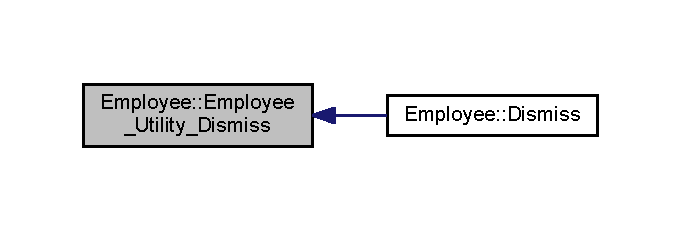
\includegraphics[width=327pt]{class_employee_a6d9c2cbf05d3137a24c322b1525fffa2_icgraph}
\end{center}
\end{figure}
\mbox{\Hypertarget{class_employee_a462e85cd69817614a7c9e030fb806f29}\label{class_employee_a462e85cd69817614a7c9e030fb806f29}} 
\index{Employee@{Employee}!Get\+Cause\+Of\+Acception@{Get\+Cause\+Of\+Acception}}
\index{Get\+Cause\+Of\+Acception@{Get\+Cause\+Of\+Acception}!Employee@{Employee}}
\subsubsection{\texorpdfstring{Get\+Cause\+Of\+Acception()}{GetCauseOfAcception()}}
{\footnotesize\ttfamily string Employee\+::\+Get\+Cause\+Of\+Acception (\begin{DoxyParamCaption}{ }\end{DoxyParamCaption})}



Definition at line 130 of file Employee.\+cpp.

Here is the caller graph for this function\+:
\nopagebreak
\begin{figure}[H]
\begin{center}
\leavevmode
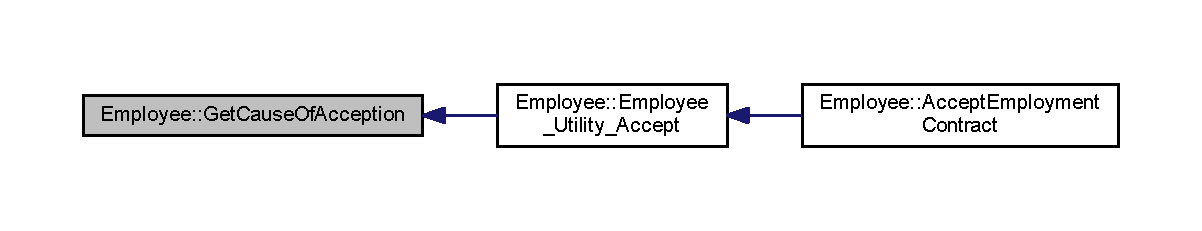
\includegraphics[width=350pt]{class_employee_a462e85cd69817614a7c9e030fb806f29_icgraph}
\end{center}
\end{figure}
\mbox{\Hypertarget{class_employee_aa7e35077b13efe6cbc362dc7b561b010}\label{class_employee_aa7e35077b13efe6cbc362dc7b561b010}} 
\index{Employee@{Employee}!Get\+Cause\+Of\+Dismission@{Get\+Cause\+Of\+Dismission}}
\index{Get\+Cause\+Of\+Dismission@{Get\+Cause\+Of\+Dismission}!Employee@{Employee}}
\subsubsection{\texorpdfstring{Get\+Cause\+Of\+Dismission()}{GetCauseOfDismission()}}
{\footnotesize\ttfamily string Employee\+::\+Get\+Cause\+Of\+Dismission (\begin{DoxyParamCaption}{ }\end{DoxyParamCaption})}



Definition at line 142 of file Employee.\+cpp.

Here is the caller graph for this function\+:
\nopagebreak
\begin{figure}[H]
\begin{center}
\leavevmode
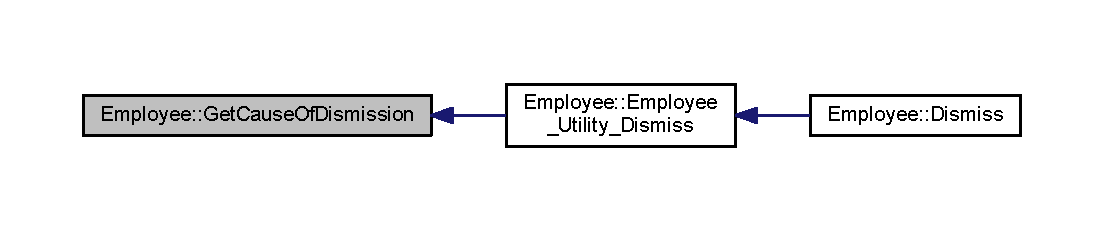
\includegraphics[width=350pt]{class_employee_aa7e35077b13efe6cbc362dc7b561b010_icgraph}
\end{center}
\end{figure}
\mbox{\Hypertarget{class_employee_ad8df9b482bc23365e06357005524c5fd}\label{class_employee_ad8df9b482bc23365e06357005524c5fd}} 
\index{Employee@{Employee}!Get\+Date\+Of\+Acception@{Get\+Date\+Of\+Acception}}
\index{Get\+Date\+Of\+Acception@{Get\+Date\+Of\+Acception}!Employee@{Employee}}
\subsubsection{\texorpdfstring{Get\+Date\+Of\+Acception()}{GetDateOfAcception()}}
{\footnotesize\ttfamily string Employee\+::\+Get\+Date\+Of\+Acception (\begin{DoxyParamCaption}{ }\end{DoxyParamCaption})}



Definition at line 126 of file Employee.\+cpp.

Here is the caller graph for this function\+:
\nopagebreak
\begin{figure}[H]
\begin{center}
\leavevmode
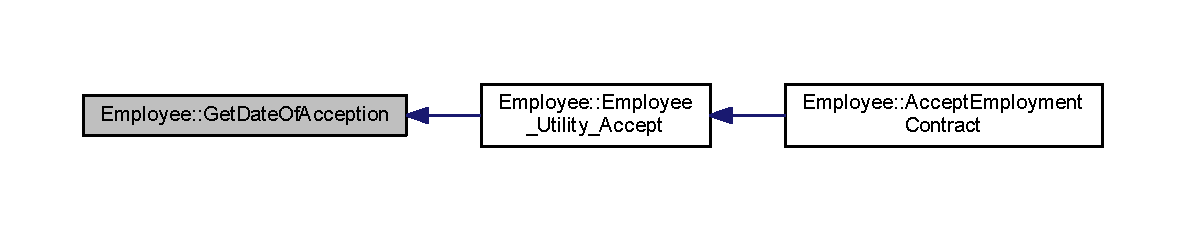
\includegraphics[width=350pt]{class_employee_ad8df9b482bc23365e06357005524c5fd_icgraph}
\end{center}
\end{figure}
\mbox{\Hypertarget{class_employee_a9bf98793dad6f452b3b99b353a4a6635}\label{class_employee_a9bf98793dad6f452b3b99b353a4a6635}} 
\index{Employee@{Employee}!Get\+Date\+Of\+Dismiss@{Get\+Date\+Of\+Dismiss}}
\index{Get\+Date\+Of\+Dismiss@{Get\+Date\+Of\+Dismiss}!Employee@{Employee}}
\subsubsection{\texorpdfstring{Get\+Date\+Of\+Dismiss()}{GetDateOfDismiss()}}
{\footnotesize\ttfamily string Employee\+::\+Get\+Date\+Of\+Dismiss (\begin{DoxyParamCaption}{ }\end{DoxyParamCaption})}



Definition at line 138 of file Employee.\+cpp.

Here is the caller graph for this function\+:
\nopagebreak
\begin{figure}[H]
\begin{center}
\leavevmode
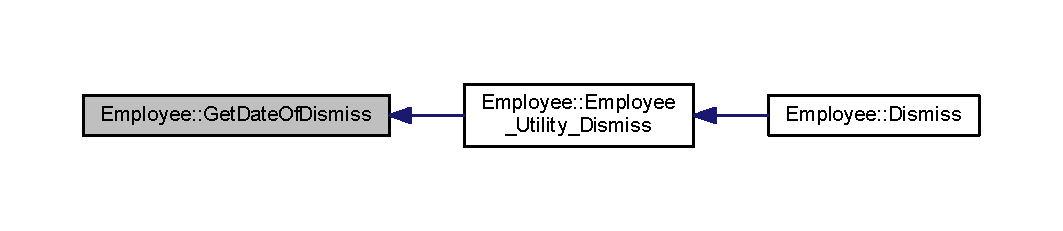
\includegraphics[width=350pt]{class_employee_a9bf98793dad6f452b3b99b353a4a6635_icgraph}
\end{center}
\end{figure}
\mbox{\Hypertarget{class_employee_a7782178746f3640942450a0f7271ef60}\label{class_employee_a7782178746f3640942450a0f7271ef60}} 
\index{Employee@{Employee}!Get\+Date\+Of\+Returning\+Money@{Get\+Date\+Of\+Returning\+Money}}
\index{Get\+Date\+Of\+Returning\+Money@{Get\+Date\+Of\+Returning\+Money}!Employee@{Employee}}
\subsubsection{\texorpdfstring{Get\+Date\+Of\+Returning\+Money()}{GetDateOfReturningMoney()}}
{\footnotesize\ttfamily string Employee\+::\+Get\+Date\+Of\+Returning\+Money (\begin{DoxyParamCaption}{ }\end{DoxyParamCaption})}



Definition at line 149 of file Employee.\+cpp.

Here is the caller graph for this function\+:
\nopagebreak
\begin{figure}[H]
\begin{center}
\leavevmode
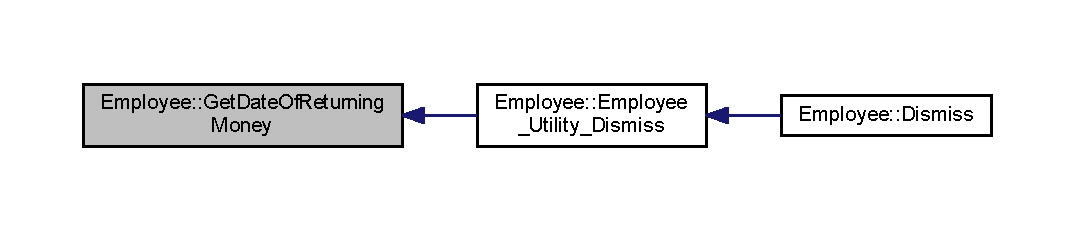
\includegraphics[width=350pt]{class_employee_a7782178746f3640942450a0f7271ef60_icgraph}
\end{center}
\end{figure}
\mbox{\Hypertarget{class_employee_ae210ea3433b4596f9d3ff5dee4c63bc2}\label{class_employee_ae210ea3433b4596f9d3ff5dee4c63bc2}} 
\index{Employee@{Employee}!Get\+New\+Position@{Get\+New\+Position}}
\index{Get\+New\+Position@{Get\+New\+Position}!Employee@{Employee}}
\subsubsection{\texorpdfstring{Get\+New\+Position()}{GetNewPosition()}}
{\footnotesize\ttfamily std\+::string Employee\+::\+Get\+New\+Position (\begin{DoxyParamCaption}\item[{void}]{ }\end{DoxyParamCaption})}



Returns new position. 



Definition at line 76 of file Employee.\+cpp.

\mbox{\Hypertarget{class_employee_a8ad22e912e2e4e336416df20480ceb54}\label{class_employee_a8ad22e912e2e4e336416df20480ceb54}} 
\index{Employee@{Employee}!Get\+Number\+Of\+Acceptional\+Order@{Get\+Number\+Of\+Acceptional\+Order}}
\index{Get\+Number\+Of\+Acceptional\+Order@{Get\+Number\+Of\+Acceptional\+Order}!Employee@{Employee}}
\subsubsection{\texorpdfstring{Get\+Number\+Of\+Acceptional\+Order()}{GetNumberOfAcceptionalOrder()}}
{\footnotesize\ttfamily int Employee\+::\+Get\+Number\+Of\+Acceptional\+Order (\begin{DoxyParamCaption}{ }\end{DoxyParamCaption})}



Definition at line 134 of file Employee.\+cpp.

Here is the caller graph for this function\+:
\nopagebreak
\begin{figure}[H]
\begin{center}
\leavevmode
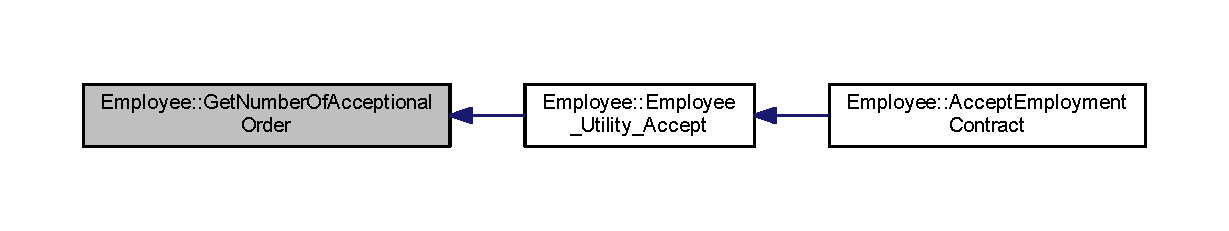
\includegraphics[width=350pt]{class_employee_a8ad22e912e2e4e336416df20480ceb54_icgraph}
\end{center}
\end{figure}
\mbox{\Hypertarget{class_employee_a521952ca263ba6ad783c634631070076}\label{class_employee_a521952ca263ba6ad783c634631070076}} 
\index{Employee@{Employee}!Get\+Number\+Of\+Dismissal\+Order@{Get\+Number\+Of\+Dismissal\+Order}}
\index{Get\+Number\+Of\+Dismissal\+Order@{Get\+Number\+Of\+Dismissal\+Order}!Employee@{Employee}}
\subsubsection{\texorpdfstring{Get\+Number\+Of\+Dismissal\+Order()}{GetNumberOfDismissalOrder()}}
{\footnotesize\ttfamily int Employee\+::\+Get\+Number\+Of\+Dismissal\+Order (\begin{DoxyParamCaption}{ }\end{DoxyParamCaption})}



Definition at line 145 of file Employee.\+cpp.

Here is the caller graph for this function\+:
\nopagebreak
\begin{figure}[H]
\begin{center}
\leavevmode
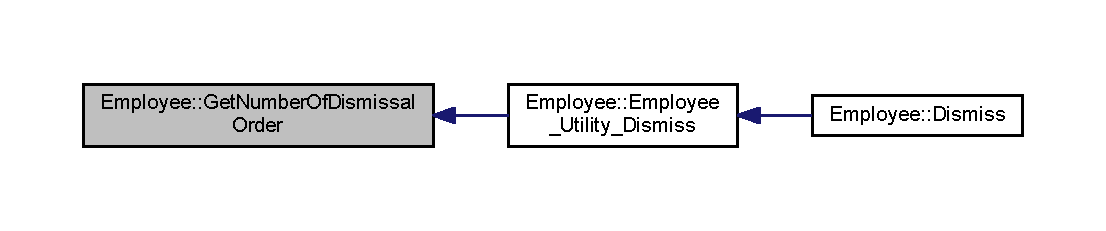
\includegraphics[width=350pt]{class_employee_a521952ca263ba6ad783c634631070076_icgraph}
\end{center}
\end{figure}
\mbox{\Hypertarget{class_employee_a37e77828f9f559a27951e3113b3fb520}\label{class_employee_a37e77828f9f559a27951e3113b3fb520}} 
\index{Employee@{Employee}!Give\+Resume@{Give\+Resume}}
\index{Give\+Resume@{Give\+Resume}!Employee@{Employee}}
\subsubsection{\texorpdfstring{Give\+Resume()}{GiveResume()}}
{\footnotesize\ttfamily std\+::string Employee\+::\+Give\+Resume (\begin{DoxyParamCaption}\item[{void}]{ }\end{DoxyParamCaption})}



Returns CV. 



Definition at line 84 of file Employee.\+cpp.

\mbox{\Hypertarget{class_employee_a8644c276b8a3cdb8bb62a71a492e574d}\label{class_employee_a8644c276b8a3cdb8bb62a71a492e574d}} 
\index{Employee@{Employee}!Go\+On\+Training\+Courses@{Go\+On\+Training\+Courses}}
\index{Go\+On\+Training\+Courses@{Go\+On\+Training\+Courses}!Employee@{Employee}}
\subsubsection{\texorpdfstring{Go\+On\+Training\+Courses()}{GoOnTrainingCourses()}}
{\footnotesize\ttfamily int Employee\+::\+Go\+On\+Training\+Courses (\begin{DoxyParamCaption}\item[{void}]{ }\end{DoxyParamCaption})}



Sends to training course. 



Definition at line 80 of file Employee.\+cpp.

\mbox{\Hypertarget{class_employee_a7eebc60f8cfd43fe07fae6196a317b0c}\label{class_employee_a7eebc60f8cfd43fe07fae6196a317b0c}} 
\index{Employee@{Employee}!Set\+Cause\+Of\+Acception@{Set\+Cause\+Of\+Acception}}
\index{Set\+Cause\+Of\+Acception@{Set\+Cause\+Of\+Acception}!Employee@{Employee}}
\subsubsection{\texorpdfstring{Set\+Cause\+Of\+Acception()}{SetCauseOfAcception()}}
{\footnotesize\ttfamily void Employee\+::\+Set\+Cause\+Of\+Acception (\begin{DoxyParamCaption}\item[{string}]{v\+\_\+\+Cause\+Of\+Acception }\end{DoxyParamCaption})}



Definition at line 102 of file Employee.\+cpp.

Here is the caller graph for this function\+:
\nopagebreak
\begin{figure}[H]
\begin{center}
\leavevmode
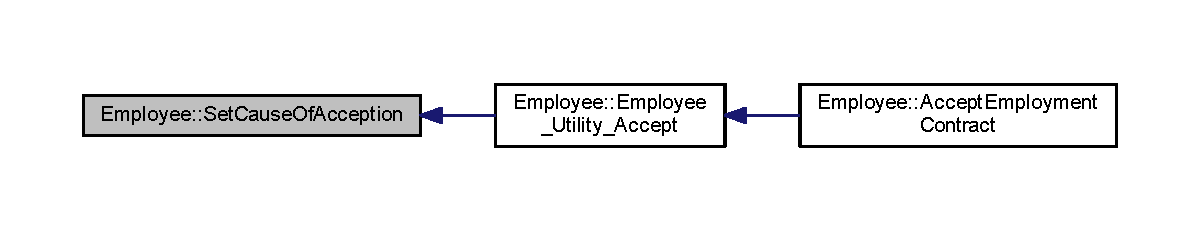
\includegraphics[width=350pt]{class_employee_a7eebc60f8cfd43fe07fae6196a317b0c_icgraph}
\end{center}
\end{figure}
\mbox{\Hypertarget{class_employee_ac129a41d2cb756360ad056bf39c25464}\label{class_employee_ac129a41d2cb756360ad056bf39c25464}} 
\index{Employee@{Employee}!Set\+Cause\+Of\+Dismission@{Set\+Cause\+Of\+Dismission}}
\index{Set\+Cause\+Of\+Dismission@{Set\+Cause\+Of\+Dismission}!Employee@{Employee}}
\subsubsection{\texorpdfstring{Set\+Cause\+Of\+Dismission()}{SetCauseOfDismission()}}
{\footnotesize\ttfamily void Employee\+::\+Set\+Cause\+Of\+Dismission (\begin{DoxyParamCaption}\item[{string}]{v\+\_\+\+Cause\+Of\+Dismission }\end{DoxyParamCaption})}



Definition at line 114 of file Employee.\+cpp.

Here is the caller graph for this function\+:
\nopagebreak
\begin{figure}[H]
\begin{center}
\leavevmode
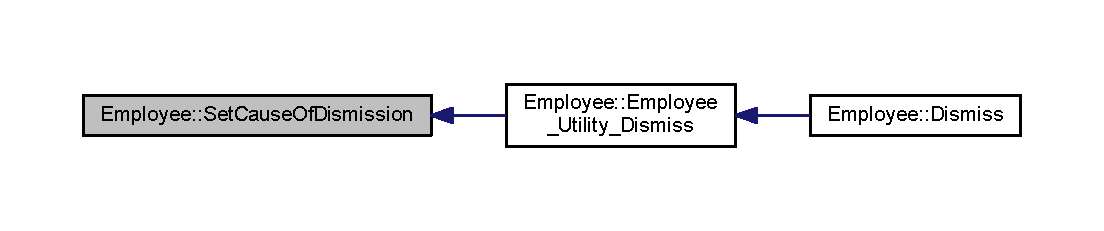
\includegraphics[width=350pt]{class_employee_ac129a41d2cb756360ad056bf39c25464_icgraph}
\end{center}
\end{figure}
\mbox{\Hypertarget{class_employee_a62cc0f19d969528e061ad178a1b109ac}\label{class_employee_a62cc0f19d969528e061ad178a1b109ac}} 
\index{Employee@{Employee}!Set\+Date\+Of\+Acception@{Set\+Date\+Of\+Acception}}
\index{Set\+Date\+Of\+Acception@{Set\+Date\+Of\+Acception}!Employee@{Employee}}
\subsubsection{\texorpdfstring{Set\+Date\+Of\+Acception()}{SetDateOfAcception()}}
{\footnotesize\ttfamily void Employee\+::\+Set\+Date\+Of\+Acception (\begin{DoxyParamCaption}\item[{string}]{v\+\_\+\+Date\+Of\+Acception }\end{DoxyParamCaption})}



Definition at line 98 of file Employee.\+cpp.

Here is the caller graph for this function\+:
\nopagebreak
\begin{figure}[H]
\begin{center}
\leavevmode
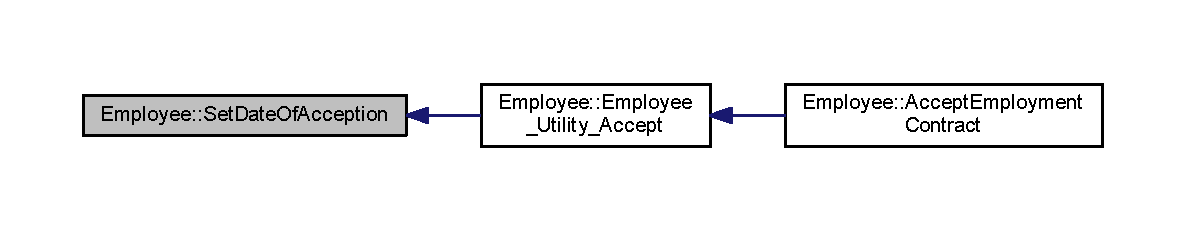
\includegraphics[width=350pt]{class_employee_a62cc0f19d969528e061ad178a1b109ac_icgraph}
\end{center}
\end{figure}
\mbox{\Hypertarget{class_employee_acbb98daeb702b22d616c8b7064784210}\label{class_employee_acbb98daeb702b22d616c8b7064784210}} 
\index{Employee@{Employee}!Set\+Date\+Of\+Dismiss@{Set\+Date\+Of\+Dismiss}}
\index{Set\+Date\+Of\+Dismiss@{Set\+Date\+Of\+Dismiss}!Employee@{Employee}}
\subsubsection{\texorpdfstring{Set\+Date\+Of\+Dismiss()}{SetDateOfDismiss()}}
{\footnotesize\ttfamily void Employee\+::\+Set\+Date\+Of\+Dismiss (\begin{DoxyParamCaption}\item[{string}]{v\+\_\+\+Date\+Of\+Dismiss }\end{DoxyParamCaption})}



Definition at line 110 of file Employee.\+cpp.

Here is the caller graph for this function\+:
\nopagebreak
\begin{figure}[H]
\begin{center}
\leavevmode
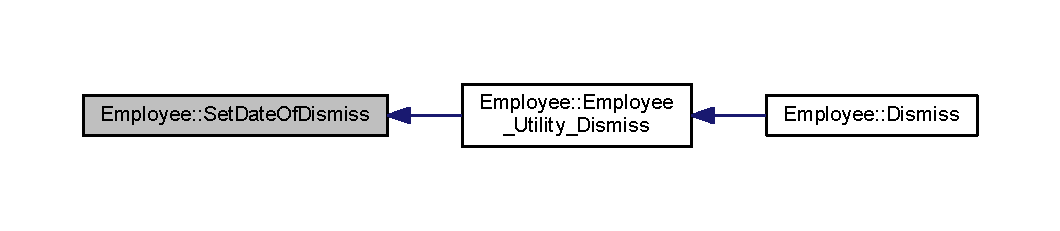
\includegraphics[width=350pt]{class_employee_acbb98daeb702b22d616c8b7064784210_icgraph}
\end{center}
\end{figure}
\mbox{\Hypertarget{class_employee_a3ffb3c8c2dc4817f88801be832eb8caa}\label{class_employee_a3ffb3c8c2dc4817f88801be832eb8caa}} 
\index{Employee@{Employee}!Set\+Date\+Of\+Returning\+Money@{Set\+Date\+Of\+Returning\+Money}}
\index{Set\+Date\+Of\+Returning\+Money@{Set\+Date\+Of\+Returning\+Money}!Employee@{Employee}}
\subsubsection{\texorpdfstring{Set\+Date\+Of\+Returning\+Money()}{SetDateOfReturningMoney()}}
{\footnotesize\ttfamily void Employee\+::\+Set\+Date\+Of\+Returning\+Money (\begin{DoxyParamCaption}\item[{string}]{v\+\_\+\+Date\+Of\+Returning\+Money }\end{DoxyParamCaption})}



Definition at line 122 of file Employee.\+cpp.

Here is the caller graph for this function\+:
\nopagebreak
\begin{figure}[H]
\begin{center}
\leavevmode
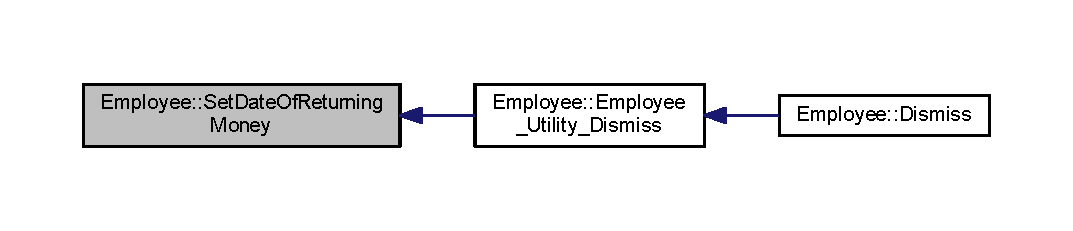
\includegraphics[width=350pt]{class_employee_a3ffb3c8c2dc4817f88801be832eb8caa_icgraph}
\end{center}
\end{figure}
\mbox{\Hypertarget{class_employee_ae0a2d5a5ec36af567bc7e434d18de422}\label{class_employee_ae0a2d5a5ec36af567bc7e434d18de422}} 
\index{Employee@{Employee}!Set\+Number\+Of\+Acceptional\+Order@{Set\+Number\+Of\+Acceptional\+Order}}
\index{Set\+Number\+Of\+Acceptional\+Order@{Set\+Number\+Of\+Acceptional\+Order}!Employee@{Employee}}
\subsubsection{\texorpdfstring{Set\+Number\+Of\+Acceptional\+Order()}{SetNumberOfAcceptionalOrder()}}
{\footnotesize\ttfamily void Employee\+::\+Set\+Number\+Of\+Acceptional\+Order (\begin{DoxyParamCaption}\item[{int}]{v\+\_\+\+Number\+Of\+Acceptional\+Order }\end{DoxyParamCaption})}



Definition at line 106 of file Employee.\+cpp.

Here is the caller graph for this function\+:
\nopagebreak
\begin{figure}[H]
\begin{center}
\leavevmode
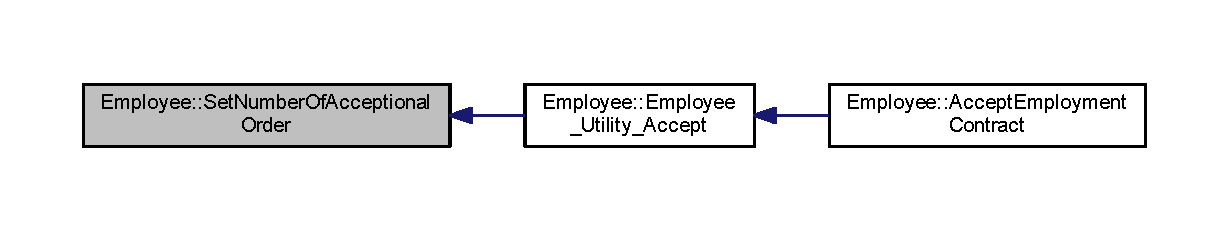
\includegraphics[width=350pt]{class_employee_ae0a2d5a5ec36af567bc7e434d18de422_icgraph}
\end{center}
\end{figure}
\mbox{\Hypertarget{class_employee_abcf46d071f43b17f0a83b00a327822b9}\label{class_employee_abcf46d071f43b17f0a83b00a327822b9}} 
\index{Employee@{Employee}!Set\+Number\+Of\+Dismissal\+Order@{Set\+Number\+Of\+Dismissal\+Order}}
\index{Set\+Number\+Of\+Dismissal\+Order@{Set\+Number\+Of\+Dismissal\+Order}!Employee@{Employee}}
\subsubsection{\texorpdfstring{Set\+Number\+Of\+Dismissal\+Order()}{SetNumberOfDismissalOrder()}}
{\footnotesize\ttfamily void Employee\+::\+Set\+Number\+Of\+Dismissal\+Order (\begin{DoxyParamCaption}\item[{int}]{v\+\_\+\+Number\+Of\+Dismissal\+Order }\end{DoxyParamCaption})}



Definition at line 118 of file Employee.\+cpp.

Here is the caller graph for this function\+:
\nopagebreak
\begin{figure}[H]
\begin{center}
\leavevmode
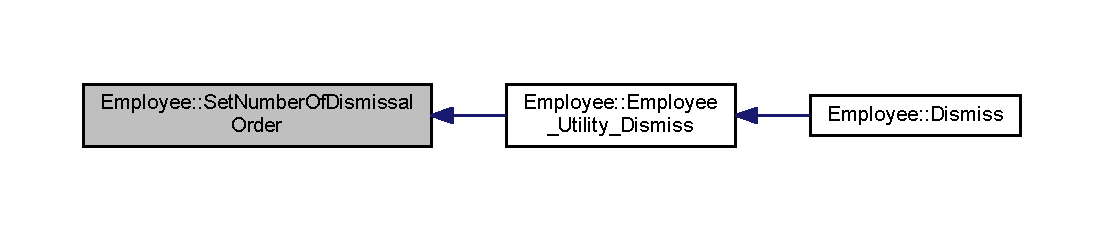
\includegraphics[width=350pt]{class_employee_abcf46d071f43b17f0a83b00a327822b9_icgraph}
\end{center}
\end{figure}


\subsection{Member Data Documentation}
\mbox{\Hypertarget{class_employee_ae218a1ea5ff298c3501afa8e815da9d7}\label{class_employee_ae218a1ea5ff298c3501afa8e815da9d7}} 
\index{Employee@{Employee}!Cause\+Of\+Acception@{Cause\+Of\+Acception}}
\index{Cause\+Of\+Acception@{Cause\+Of\+Acception}!Employee@{Employee}}
\subsubsection{\texorpdfstring{Cause\+Of\+Acception}{CauseOfAcception}}
{\footnotesize\ttfamily string Employee\+::\+Cause\+Of\+Acception\hspace{0.3cm}{\ttfamily [private]}}



Definition at line 57 of file Employee.\+h.

\mbox{\Hypertarget{class_employee_a80bd5a84291a0369521af1dcfecca970}\label{class_employee_a80bd5a84291a0369521af1dcfecca970}} 
\index{Employee@{Employee}!Cause\+Of\+Dismission@{Cause\+Of\+Dismission}}
\index{Cause\+Of\+Dismission@{Cause\+Of\+Dismission}!Employee@{Employee}}
\subsubsection{\texorpdfstring{Cause\+Of\+Dismission}{CauseOfDismission}}
{\footnotesize\ttfamily string Employee\+::\+Cause\+Of\+Dismission\hspace{0.3cm}{\ttfamily [private]}}



Definition at line 60 of file Employee.\+h.

\mbox{\Hypertarget{class_employee_a4b6f93cebcc5e3bb343f89d65467c4d2}\label{class_employee_a4b6f93cebcc5e3bb343f89d65467c4d2}} 
\index{Employee@{Employee}!Date\+Of\+Acception@{Date\+Of\+Acception}}
\index{Date\+Of\+Acception@{Date\+Of\+Acception}!Employee@{Employee}}
\subsubsection{\texorpdfstring{Date\+Of\+Acception}{DateOfAcception}}
{\footnotesize\ttfamily string Employee\+::\+Date\+Of\+Acception\hspace{0.3cm}{\ttfamily [private]}}



Definition at line 56 of file Employee.\+h.

\mbox{\Hypertarget{class_employee_a1402b4d32163d3fca601082052d2ff80}\label{class_employee_a1402b4d32163d3fca601082052d2ff80}} 
\index{Employee@{Employee}!Date\+Of\+Dismiss@{Date\+Of\+Dismiss}}
\index{Date\+Of\+Dismiss@{Date\+Of\+Dismiss}!Employee@{Employee}}
\subsubsection{\texorpdfstring{Date\+Of\+Dismiss}{DateOfDismiss}}
{\footnotesize\ttfamily string Employee\+::\+Date\+Of\+Dismiss\hspace{0.3cm}{\ttfamily [private]}}



Definition at line 59 of file Employee.\+h.

\mbox{\Hypertarget{class_employee_a05233437fad4de82175600c04552f0ca}\label{class_employee_a05233437fad4de82175600c04552f0ca}} 
\index{Employee@{Employee}!Date\+Of\+Returning\+Money@{Date\+Of\+Returning\+Money}}
\index{Date\+Of\+Returning\+Money@{Date\+Of\+Returning\+Money}!Employee@{Employee}}
\subsubsection{\texorpdfstring{Date\+Of\+Returning\+Money}{DateOfReturningMoney}}
{\footnotesize\ttfamily string Employee\+::\+Date\+Of\+Returning\+Money\hspace{0.3cm}{\ttfamily [private]}}



Definition at line 62 of file Employee.\+h.

\mbox{\Hypertarget{class_employee_aafefc3b0042fe3cf88dff13a6458e5de}\label{class_employee_aafefc3b0042fe3cf88dff13a6458e5de}} 
\index{Employee@{Employee}!Number\+Of\+Acceptional\+Order@{Number\+Of\+Acceptional\+Order}}
\index{Number\+Of\+Acceptional\+Order@{Number\+Of\+Acceptional\+Order}!Employee@{Employee}}
\subsubsection{\texorpdfstring{Number\+Of\+Acceptional\+Order}{NumberOfAcceptionalOrder}}
{\footnotesize\ttfamily int Employee\+::\+Number\+Of\+Acceptional\+Order\hspace{0.3cm}{\ttfamily [private]}}



Definition at line 58 of file Employee.\+h.

\mbox{\Hypertarget{class_employee_a0dc06d409299d253f240ceb01d1a3faf}\label{class_employee_a0dc06d409299d253f240ceb01d1a3faf}} 
\index{Employee@{Employee}!Number\+Of\+Dismissal\+Order@{Number\+Of\+Dismissal\+Order}}
\index{Number\+Of\+Dismissal\+Order@{Number\+Of\+Dismissal\+Order}!Employee@{Employee}}
\subsubsection{\texorpdfstring{Number\+Of\+Dismissal\+Order}{NumberOfDismissalOrder}}
{\footnotesize\ttfamily int Employee\+::\+Number\+Of\+Dismissal\+Order\hspace{0.3cm}{\ttfamily [private]}}



Definition at line 61 of file Employee.\+h.

\mbox{\Hypertarget{class_employee_a3a0668e43e943ba0ac0ad0470de8599a}\label{class_employee_a3a0668e43e943ba0ac0ad0470de8599a}} 
\index{Employee@{Employee}!personal\+Card@{personal\+Card}}
\index{personal\+Card@{personal\+Card}!Employee@{Employee}}
\subsubsection{\texorpdfstring{personal\+Card}{personalCard}}
{\footnotesize\ttfamily \hyperlink{class_personal_card}{Personal\+Card} Employee\+::personal\+Card\hspace{0.3cm}{\ttfamily [private]}}



Definition at line 65 of file Employee.\+h.



The documentation for this class was generated from the following files\+:\begin{DoxyCompactItemize}
\item 
C\+:/\+Workspace/\+I\+T\+Company\+Cpp/\+I\+T\+Company/\+I\+T\+Company/\hyperlink{_employee_8h}{Employee.\+h}\item 
C\+:/\+Workspace/\+I\+T\+Company\+Cpp/\+I\+T\+Company/\+I\+T\+Company/\hyperlink{_employee_8cpp}{Employee.\+cpp}\end{DoxyCompactItemize}

\hypertarget{class_h_r}{}\section{HR Class Reference}
\label{class_h_r}\index{HR@{HR}}


\hyperlink{class_h_r}{HR} class.  




{\ttfamily \#include $<$H\+R.\+h$>$}

\subsection*{Public Member Functions}
\begin{DoxyCompactItemize}
\item 
\hyperlink{class_h_r_a0cb187ef9d2c057d44e9bfcb679eed27}{HR} ()
\begin{DoxyCompactList}\small\item\em Default constructor. \end{DoxyCompactList}\item 
\hyperlink{class_h_r_a23fb380ea282a4193a7f05f81506c779}{$\sim$\+HR} ()
\begin{DoxyCompactList}\small\item\em Destructor. \end{DoxyCompactList}\item 
string \hyperlink{class_h_r_a3c509dc4449f8406ebd4bac482a8b50c}{Write\+Order\+In\+Personal\+Card} (int i)
\item 
int \hyperlink{class_h_r_af3a791db3d60be02234605865c0979da}{Allow\+To\+Go\+On\+Business\+Trip} (void)
\item 
int \hyperlink{class_h_r_a1a6f8313fedc1e0ad25827b35cb80427}{Allow\+To\+Go\+On\+Training\+Courses} (void)
\item 
int \hyperlink{class_h_r_a890c8452142fee7556b7498785f10b6f}{Allow\+To\+Go\+On\+Vacation} (void)
\item 
int \hyperlink{class_h_r_a7f7c6e9ee2f6010fbf53ceb94d18ddfb}{Allow\+To\+Take\+The\+Hospital} (void)
\item 
string \hyperlink{class_h_r_a0047e05a0a5ebee5dfafe50fe61ee373}{Return\+Docs} (int i)
\item 
string \hyperlink{class_h_r_ad794de5aee2a01b9ac3d5f22d435afba}{Giving\+A\+Changes\+In\+Personal\+Cardof\+Worker} ()
\item 
string \hyperlink{class_h_r_a3f962907d6ed8e81da66d4608ff3660d}{Putting\+Mark\+Of\+Reckoning\+In\+Employment\+History\+Book} (void)
\item 
string \hyperlink{class_h_r_a896d89581c96f0dcedca7440d2798d15}{Adding\+To\+A\+Personal\+Card\+Mark\+That\+Documents\+Are\+Returned} (void)
\item 
string \hyperlink{class_h_r_aacf64628213ae72aa5ff5a1b44e829fa}{Putting\+A\+Mark\+In\+Employment\+History\+Book} (void)
\item 
void \hyperlink{class_h_r_a795d089594c22910ea58938faf131b67}{Set\+Firstname} (string v\+\_\+\+Firstname)
\item 
void \hyperlink{class_h_r_ae092262d1dc245604fdb37fbe5564362}{Set\+Position} (string v\+\_\+\+Position)
\item 
void \hyperlink{class_h_r_ac927323d22c1580b0b6d258e28294322}{Set\+Is\+Ordered} (bool v\+\_\+\+Is\+Ordered)
\item 
string \hyperlink{class_h_r_a03a185de9601109b13c6a34c381b7b6f}{Get\+Firstname} ()
\item 
string \hyperlink{class_h_r_aed5b4581248646ba06467442b080c262}{Get\+Position} ()
\item 
bool \hyperlink{class_h_r_acbee31efce04c45b16cd9f24c7e2359c}{Get\+Is\+Ordered} ()
\item 
bool \hyperlink{class_h_r_af2203b0b515794db46c12b02bc9b9bd2}{Check\+Is\+Ordered} (bool is\+Ordered)
\end{DoxyCompactItemize}
\subsection*{Private Member Functions}
\begin{DoxyCompactItemize}
\item 
string \hyperlink{class_h_r_a55cb339b18d5eac3fb3a7a9a260d5f98}{H\+R\+\_\+\+Utility} (int i)
\begin{DoxyCompactList}\small\item\em utility funtioin \end{DoxyCompactList}\end{DoxyCompactItemize}
\subsection*{Private Attributes}
\begin{DoxyCompactItemize}
\item 
string \hyperlink{class_h_r_a9d6a324bfb9253c23e71eefeb8bacde2}{Firstname}
\begin{DoxyCompactList}\small\item\em first name \end{DoxyCompactList}\item 
string \hyperlink{class_h_r_aa19b0e239c73c6f5ab18801f102f1c2e}{Position}
\begin{DoxyCompactList}\small\item\em position \end{DoxyCompactList}\item 
bool \hyperlink{class_h_r_a9afdecc986cdc4e15a8d73b30286dbdc}{Is\+Ordered}
\begin{DoxyCompactList}\small\item\em is ordered \end{DoxyCompactList}\item 
vector$<$ \hyperlink{class_documents}{Documents} $>$ \hyperlink{class_h_r_a3dca2f7facc0c01c245af8a1a1994f37}{docs}
\begin{DoxyCompactList}\small\item\em contains \hyperlink{class_documents}{Documents} \end{DoxyCompactList}\end{DoxyCompactItemize}


\subsection{Detailed Description}
\hyperlink{class_h_r}{HR} class. 

Definition at line 15 of file H\+R.\+h.



\subsection{Constructor \& Destructor Documentation}
\mbox{\Hypertarget{class_h_r_a0cb187ef9d2c057d44e9bfcb679eed27}\label{class_h_r_a0cb187ef9d2c057d44e9bfcb679eed27}} 
\index{HR@{HR}!HR@{HR}}
\index{HR@{HR}!HR@{HR}}
\subsubsection{\texorpdfstring{H\+R()}{HR()}}
{\footnotesize\ttfamily H\+R\+::\+HR (\begin{DoxyParamCaption}{ }\end{DoxyParamCaption})}



Default constructor. 



Definition at line 3 of file H\+R.\+cpp.

\mbox{\Hypertarget{class_h_r_a23fb380ea282a4193a7f05f81506c779}\label{class_h_r_a23fb380ea282a4193a7f05f81506c779}} 
\index{HR@{HR}!````~HR@{$\sim$\+HR}}
\index{````~HR@{$\sim$\+HR}!HR@{HR}}
\subsubsection{\texorpdfstring{$\sim$\+H\+R()}{~HR()}}
{\footnotesize\ttfamily H\+R\+::$\sim$\+HR (\begin{DoxyParamCaption}{ }\end{DoxyParamCaption})}



Destructor. 



Definition at line 7 of file H\+R.\+cpp.



\subsection{Member Function Documentation}
\mbox{\Hypertarget{class_h_r_a896d89581c96f0dcedca7440d2798d15}\label{class_h_r_a896d89581c96f0dcedca7440d2798d15}} 
\index{HR@{HR}!Adding\+To\+A\+Personal\+Card\+Mark\+That\+Documents\+Are\+Returned@{Adding\+To\+A\+Personal\+Card\+Mark\+That\+Documents\+Are\+Returned}}
\index{Adding\+To\+A\+Personal\+Card\+Mark\+That\+Documents\+Are\+Returned@{Adding\+To\+A\+Personal\+Card\+Mark\+That\+Documents\+Are\+Returned}!HR@{HR}}
\subsubsection{\texorpdfstring{Adding\+To\+A\+Personal\+Card\+Mark\+That\+Documents\+Are\+Returned()}{AddingToAPersonalCardMarkThatDocumentsAreReturned()}}
{\footnotesize\ttfamily std\+::string H\+R\+::\+Adding\+To\+A\+Personal\+Card\+Mark\+That\+Documents\+Are\+Returned (\begin{DoxyParamCaption}\item[{void}]{ }\end{DoxyParamCaption})}



Definition at line 64 of file H\+R.\+cpp.

\mbox{\Hypertarget{class_h_r_af3a791db3d60be02234605865c0979da}\label{class_h_r_af3a791db3d60be02234605865c0979da}} 
\index{HR@{HR}!Allow\+To\+Go\+On\+Business\+Trip@{Allow\+To\+Go\+On\+Business\+Trip}}
\index{Allow\+To\+Go\+On\+Business\+Trip@{Allow\+To\+Go\+On\+Business\+Trip}!HR@{HR}}
\subsubsection{\texorpdfstring{Allow\+To\+Go\+On\+Business\+Trip()}{AllowToGoOnBusinessTrip()}}
{\footnotesize\ttfamily int H\+R\+::\+Allow\+To\+Go\+On\+Business\+Trip (\begin{DoxyParamCaption}\item[{void}]{ }\end{DoxyParamCaption})}



Definition at line 29 of file H\+R.\+cpp.

\mbox{\Hypertarget{class_h_r_a1a6f8313fedc1e0ad25827b35cb80427}\label{class_h_r_a1a6f8313fedc1e0ad25827b35cb80427}} 
\index{HR@{HR}!Allow\+To\+Go\+On\+Training\+Courses@{Allow\+To\+Go\+On\+Training\+Courses}}
\index{Allow\+To\+Go\+On\+Training\+Courses@{Allow\+To\+Go\+On\+Training\+Courses}!HR@{HR}}
\subsubsection{\texorpdfstring{Allow\+To\+Go\+On\+Training\+Courses()}{AllowToGoOnTrainingCourses()}}
{\footnotesize\ttfamily int H\+R\+::\+Allow\+To\+Go\+On\+Training\+Courses (\begin{DoxyParamCaption}\item[{void}]{ }\end{DoxyParamCaption})}



Definition at line 34 of file H\+R.\+cpp.

\mbox{\Hypertarget{class_h_r_a890c8452142fee7556b7498785f10b6f}\label{class_h_r_a890c8452142fee7556b7498785f10b6f}} 
\index{HR@{HR}!Allow\+To\+Go\+On\+Vacation@{Allow\+To\+Go\+On\+Vacation}}
\index{Allow\+To\+Go\+On\+Vacation@{Allow\+To\+Go\+On\+Vacation}!HR@{HR}}
\subsubsection{\texorpdfstring{Allow\+To\+Go\+On\+Vacation()}{AllowToGoOnVacation()}}
{\footnotesize\ttfamily int H\+R\+::\+Allow\+To\+Go\+On\+Vacation (\begin{DoxyParamCaption}\item[{void}]{ }\end{DoxyParamCaption})}



Definition at line 39 of file H\+R.\+cpp.

\mbox{\Hypertarget{class_h_r_a7f7c6e9ee2f6010fbf53ceb94d18ddfb}\label{class_h_r_a7f7c6e9ee2f6010fbf53ceb94d18ddfb}} 
\index{HR@{HR}!Allow\+To\+Take\+The\+Hospital@{Allow\+To\+Take\+The\+Hospital}}
\index{Allow\+To\+Take\+The\+Hospital@{Allow\+To\+Take\+The\+Hospital}!HR@{HR}}
\subsubsection{\texorpdfstring{Allow\+To\+Take\+The\+Hospital()}{AllowToTakeTheHospital()}}
{\footnotesize\ttfamily int H\+R\+::\+Allow\+To\+Take\+The\+Hospital (\begin{DoxyParamCaption}\item[{void}]{ }\end{DoxyParamCaption})}



Definition at line 44 of file H\+R.\+cpp.

\mbox{\Hypertarget{class_h_r_af2203b0b515794db46c12b02bc9b9bd2}\label{class_h_r_af2203b0b515794db46c12b02bc9b9bd2}} 
\index{HR@{HR}!Check\+Is\+Ordered@{Check\+Is\+Ordered}}
\index{Check\+Is\+Ordered@{Check\+Is\+Ordered}!HR@{HR}}
\subsubsection{\texorpdfstring{Check\+Is\+Ordered()}{CheckIsOrdered()}}
{\footnotesize\ttfamily bool H\+R\+::\+Check\+Is\+Ordered (\begin{DoxyParamCaption}\item[{bool}]{is\+Ordered }\end{DoxyParamCaption})}



Definition at line 97 of file H\+R.\+cpp.

Here is the caller graph for this function\+:
\nopagebreak
\begin{figure}[H]
\begin{center}
\leavevmode
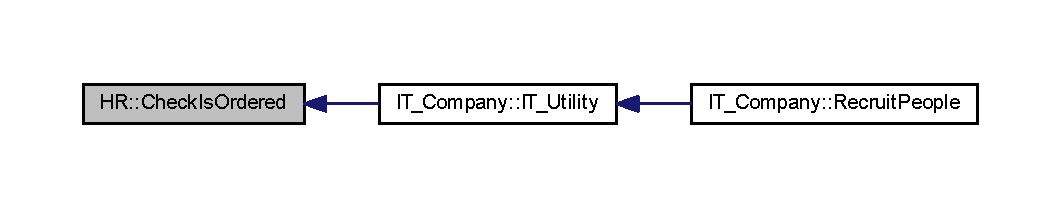
\includegraphics[width=350pt]{class_h_r_af2203b0b515794db46c12b02bc9b9bd2_icgraph}
\end{center}
\end{figure}
\mbox{\Hypertarget{class_h_r_a03a185de9601109b13c6a34c381b7b6f}\label{class_h_r_a03a185de9601109b13c6a34c381b7b6f}} 
\index{HR@{HR}!Get\+Firstname@{Get\+Firstname}}
\index{Get\+Firstname@{Get\+Firstname}!HR@{HR}}
\subsubsection{\texorpdfstring{Get\+Firstname()}{GetFirstname()}}
{\footnotesize\ttfamily string H\+R\+::\+Get\+Firstname (\begin{DoxyParamCaption}{ }\end{DoxyParamCaption})}



Definition at line 85 of file H\+R.\+cpp.

Here is the caller graph for this function\+:
\nopagebreak
\begin{figure}[H]
\begin{center}
\leavevmode
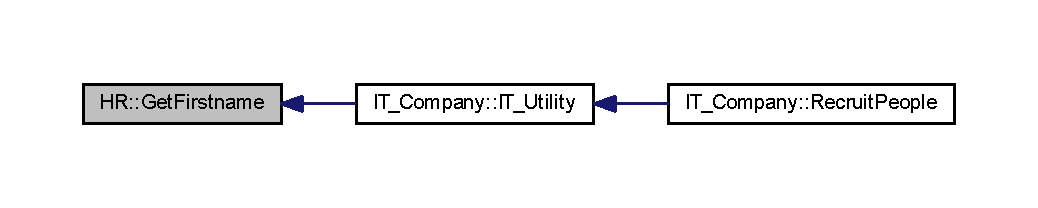
\includegraphics[width=350pt]{class_h_r_a03a185de9601109b13c6a34c381b7b6f_icgraph}
\end{center}
\end{figure}
\mbox{\Hypertarget{class_h_r_acbee31efce04c45b16cd9f24c7e2359c}\label{class_h_r_acbee31efce04c45b16cd9f24c7e2359c}} 
\index{HR@{HR}!Get\+Is\+Ordered@{Get\+Is\+Ordered}}
\index{Get\+Is\+Ordered@{Get\+Is\+Ordered}!HR@{HR}}
\subsubsection{\texorpdfstring{Get\+Is\+Ordered()}{GetIsOrdered()}}
{\footnotesize\ttfamily bool H\+R\+::\+Get\+Is\+Ordered (\begin{DoxyParamCaption}{ }\end{DoxyParamCaption})}



Definition at line 93 of file H\+R.\+cpp.

Here is the caller graph for this function\+:
\nopagebreak
\begin{figure}[H]
\begin{center}
\leavevmode
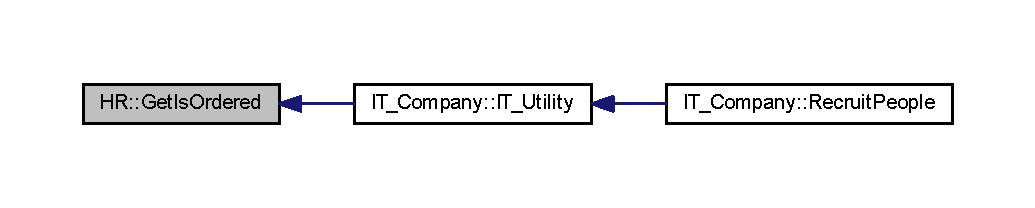
\includegraphics[width=350pt]{class_h_r_acbee31efce04c45b16cd9f24c7e2359c_icgraph}
\end{center}
\end{figure}
\mbox{\Hypertarget{class_h_r_aed5b4581248646ba06467442b080c262}\label{class_h_r_aed5b4581248646ba06467442b080c262}} 
\index{HR@{HR}!Get\+Position@{Get\+Position}}
\index{Get\+Position@{Get\+Position}!HR@{HR}}
\subsubsection{\texorpdfstring{Get\+Position()}{GetPosition()}}
{\footnotesize\ttfamily string H\+R\+::\+Get\+Position (\begin{DoxyParamCaption}{ }\end{DoxyParamCaption})}



Definition at line 89 of file H\+R.\+cpp.

Here is the caller graph for this function\+:
\nopagebreak
\begin{figure}[H]
\begin{center}
\leavevmode
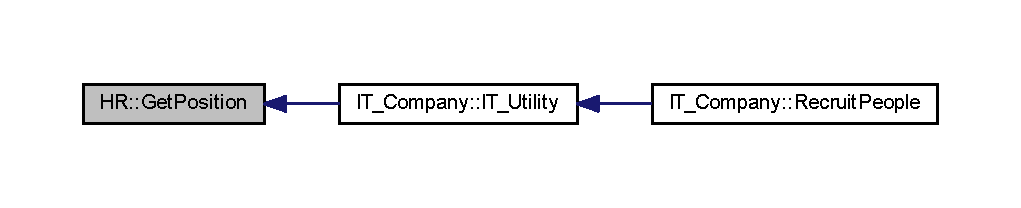
\includegraphics[width=350pt]{class_h_r_aed5b4581248646ba06467442b080c262_icgraph}
\end{center}
\end{figure}
\mbox{\Hypertarget{class_h_r_ad794de5aee2a01b9ac3d5f22d435afba}\label{class_h_r_ad794de5aee2a01b9ac3d5f22d435afba}} 
\index{HR@{HR}!Giving\+A\+Changes\+In\+Personal\+Cardof\+Worker@{Giving\+A\+Changes\+In\+Personal\+Cardof\+Worker}}
\index{Giving\+A\+Changes\+In\+Personal\+Cardof\+Worker@{Giving\+A\+Changes\+In\+Personal\+Cardof\+Worker}!HR@{HR}}
\subsubsection{\texorpdfstring{Giving\+A\+Changes\+In\+Personal\+Cardof\+Worker()}{GivingAChangesInPersonalCardofWorker()}}
{\footnotesize\ttfamily std\+::string H\+R\+::\+Giving\+A\+Changes\+In\+Personal\+Cardof\+Worker (\begin{DoxyParamCaption}{ }\end{DoxyParamCaption})}



Definition at line 54 of file H\+R.\+cpp.

\mbox{\Hypertarget{class_h_r_a55cb339b18d5eac3fb3a7a9a260d5f98}\label{class_h_r_a55cb339b18d5eac3fb3a7a9a260d5f98}} 
\index{HR@{HR}!H\+R\+\_\+\+Utility@{H\+R\+\_\+\+Utility}}
\index{H\+R\+\_\+\+Utility@{H\+R\+\_\+\+Utility}!HR@{HR}}
\subsubsection{\texorpdfstring{H\+R\+\_\+\+Utility()}{HR\_Utility()}}
{\footnotesize\ttfamily string H\+R\+::\+H\+R\+\_\+\+Utility (\begin{DoxyParamCaption}\item[{int}]{i }\end{DoxyParamCaption})\hspace{0.3cm}{\ttfamily [private]}}



utility funtioin 



Definition at line 11 of file H\+R.\+cpp.

Here is the caller graph for this function\+:
\nopagebreak
\begin{figure}[H]
\begin{center}
\leavevmode
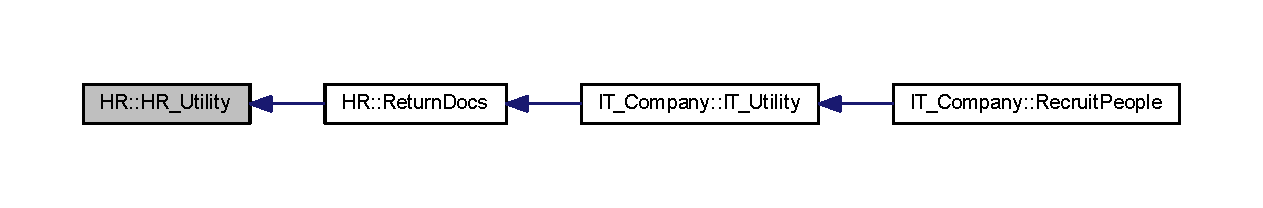
\includegraphics[width=350pt]{class_h_r_a55cb339b18d5eac3fb3a7a9a260d5f98_icgraph}
\end{center}
\end{figure}
\mbox{\Hypertarget{class_h_r_aacf64628213ae72aa5ff5a1b44e829fa}\label{class_h_r_aacf64628213ae72aa5ff5a1b44e829fa}} 
\index{HR@{HR}!Putting\+A\+Mark\+In\+Employment\+History\+Book@{Putting\+A\+Mark\+In\+Employment\+History\+Book}}
\index{Putting\+A\+Mark\+In\+Employment\+History\+Book@{Putting\+A\+Mark\+In\+Employment\+History\+Book}!HR@{HR}}
\subsubsection{\texorpdfstring{Putting\+A\+Mark\+In\+Employment\+History\+Book()}{PuttingAMarkInEmploymentHistoryBook()}}
{\footnotesize\ttfamily std\+::string H\+R\+::\+Putting\+A\+Mark\+In\+Employment\+History\+Book (\begin{DoxyParamCaption}\item[{void}]{ }\end{DoxyParamCaption})}



Definition at line 69 of file H\+R.\+cpp.

\mbox{\Hypertarget{class_h_r_a3f962907d6ed8e81da66d4608ff3660d}\label{class_h_r_a3f962907d6ed8e81da66d4608ff3660d}} 
\index{HR@{HR}!Putting\+Mark\+Of\+Reckoning\+In\+Employment\+History\+Book@{Putting\+Mark\+Of\+Reckoning\+In\+Employment\+History\+Book}}
\index{Putting\+Mark\+Of\+Reckoning\+In\+Employment\+History\+Book@{Putting\+Mark\+Of\+Reckoning\+In\+Employment\+History\+Book}!HR@{HR}}
\subsubsection{\texorpdfstring{Putting\+Mark\+Of\+Reckoning\+In\+Employment\+History\+Book()}{PuttingMarkOfReckoningInEmploymentHistoryBook()}}
{\footnotesize\ttfamily std\+::string H\+R\+::\+Putting\+Mark\+Of\+Reckoning\+In\+Employment\+History\+Book (\begin{DoxyParamCaption}\item[{void}]{ }\end{DoxyParamCaption})}



Definition at line 59 of file H\+R.\+cpp.

\mbox{\Hypertarget{class_h_r_a0047e05a0a5ebee5dfafe50fe61ee373}\label{class_h_r_a0047e05a0a5ebee5dfafe50fe61ee373}} 
\index{HR@{HR}!Return\+Docs@{Return\+Docs}}
\index{Return\+Docs@{Return\+Docs}!HR@{HR}}
\subsubsection{\texorpdfstring{Return\+Docs()}{ReturnDocs()}}
{\footnotesize\ttfamily std\+::string H\+R\+::\+Return\+Docs (\begin{DoxyParamCaption}\item[{int}]{i }\end{DoxyParamCaption})}



Definition at line 49 of file H\+R.\+cpp.

Here is the call graph for this function\+:
\nopagebreak
\begin{figure}[H]
\begin{center}
\leavevmode
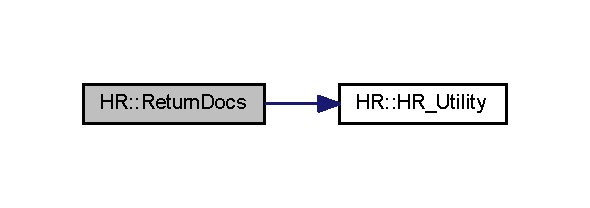
\includegraphics[width=283pt]{class_h_r_a0047e05a0a5ebee5dfafe50fe61ee373_cgraph}
\end{center}
\end{figure}
Here is the caller graph for this function\+:
\nopagebreak
\begin{figure}[H]
\begin{center}
\leavevmode
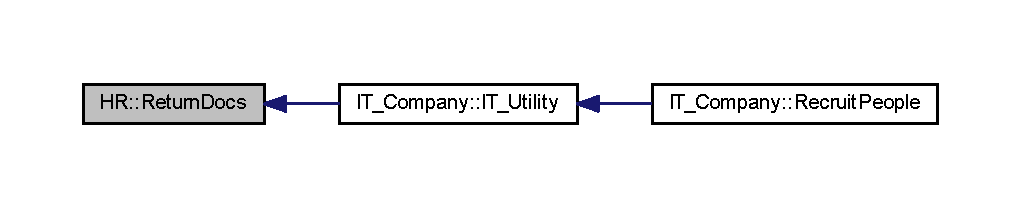
\includegraphics[width=350pt]{class_h_r_a0047e05a0a5ebee5dfafe50fe61ee373_icgraph}
\end{center}
\end{figure}
\mbox{\Hypertarget{class_h_r_a795d089594c22910ea58938faf131b67}\label{class_h_r_a795d089594c22910ea58938faf131b67}} 
\index{HR@{HR}!Set\+Firstname@{Set\+Firstname}}
\index{Set\+Firstname@{Set\+Firstname}!HR@{HR}}
\subsubsection{\texorpdfstring{Set\+Firstname()}{SetFirstname()}}
{\footnotesize\ttfamily void H\+R\+::\+Set\+Firstname (\begin{DoxyParamCaption}\item[{string}]{v\+\_\+\+Firstname }\end{DoxyParamCaption})}



Definition at line 73 of file H\+R.\+cpp.

Here is the caller graph for this function\+:
\nopagebreak
\begin{figure}[H]
\begin{center}
\leavevmode
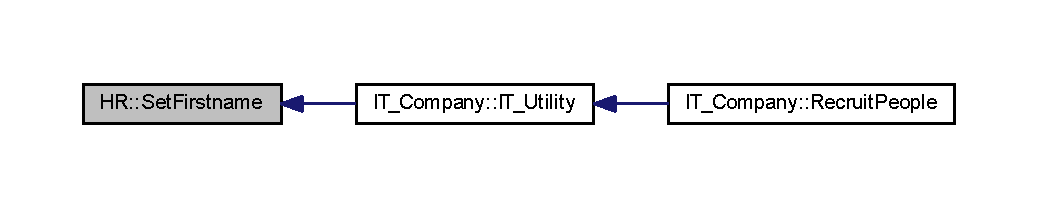
\includegraphics[width=350pt]{class_h_r_a795d089594c22910ea58938faf131b67_icgraph}
\end{center}
\end{figure}
\mbox{\Hypertarget{class_h_r_ac927323d22c1580b0b6d258e28294322}\label{class_h_r_ac927323d22c1580b0b6d258e28294322}} 
\index{HR@{HR}!Set\+Is\+Ordered@{Set\+Is\+Ordered}}
\index{Set\+Is\+Ordered@{Set\+Is\+Ordered}!HR@{HR}}
\subsubsection{\texorpdfstring{Set\+Is\+Ordered()}{SetIsOrdered()}}
{\footnotesize\ttfamily void H\+R\+::\+Set\+Is\+Ordered (\begin{DoxyParamCaption}\item[{bool}]{v\+\_\+\+Is\+Ordered }\end{DoxyParamCaption})}



Definition at line 81 of file H\+R.\+cpp.

Here is the caller graph for this function\+:
\nopagebreak
\begin{figure}[H]
\begin{center}
\leavevmode
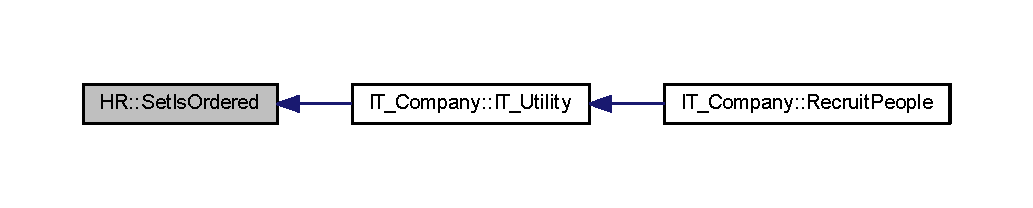
\includegraphics[width=350pt]{class_h_r_ac927323d22c1580b0b6d258e28294322_icgraph}
\end{center}
\end{figure}
\mbox{\Hypertarget{class_h_r_ae092262d1dc245604fdb37fbe5564362}\label{class_h_r_ae092262d1dc245604fdb37fbe5564362}} 
\index{HR@{HR}!Set\+Position@{Set\+Position}}
\index{Set\+Position@{Set\+Position}!HR@{HR}}
\subsubsection{\texorpdfstring{Set\+Position()}{SetPosition()}}
{\footnotesize\ttfamily void H\+R\+::\+Set\+Position (\begin{DoxyParamCaption}\item[{string}]{v\+\_\+\+Position }\end{DoxyParamCaption})}



Definition at line 77 of file H\+R.\+cpp.

Here is the caller graph for this function\+:
\nopagebreak
\begin{figure}[H]
\begin{center}
\leavevmode
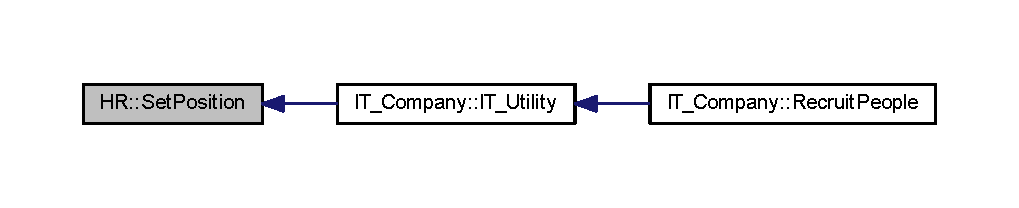
\includegraphics[width=350pt]{class_h_r_ae092262d1dc245604fdb37fbe5564362_icgraph}
\end{center}
\end{figure}
\mbox{\Hypertarget{class_h_r_a3c509dc4449f8406ebd4bac482a8b50c}\label{class_h_r_a3c509dc4449f8406ebd4bac482a8b50c}} 
\index{HR@{HR}!Write\+Order\+In\+Personal\+Card@{Write\+Order\+In\+Personal\+Card}}
\index{Write\+Order\+In\+Personal\+Card@{Write\+Order\+In\+Personal\+Card}!HR@{HR}}
\subsubsection{\texorpdfstring{Write\+Order\+In\+Personal\+Card()}{WriteOrderInPersonalCard()}}
{\footnotesize\ttfamily std\+::string H\+R\+::\+Write\+Order\+In\+Personal\+Card (\begin{DoxyParamCaption}\item[{int}]{i }\end{DoxyParamCaption})}



Definition at line 19 of file H\+R.\+cpp.

Here is the caller graph for this function\+:
\nopagebreak
\begin{figure}[H]
\begin{center}
\leavevmode
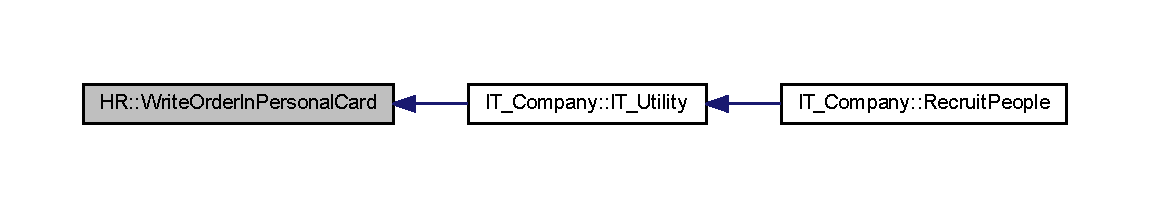
\includegraphics[width=350pt]{class_h_r_a3c509dc4449f8406ebd4bac482a8b50c_icgraph}
\end{center}
\end{figure}


\subsection{Member Data Documentation}
\mbox{\Hypertarget{class_h_r_a3dca2f7facc0c01c245af8a1a1994f37}\label{class_h_r_a3dca2f7facc0c01c245af8a1a1994f37}} 
\index{HR@{HR}!docs@{docs}}
\index{docs@{docs}!HR@{HR}}
\subsubsection{\texorpdfstring{docs}{docs}}
{\footnotesize\ttfamily vector$<$\hyperlink{class_documents}{Documents}$>$ H\+R\+::docs\hspace{0.3cm}{\ttfamily [private]}}



contains \hyperlink{class_documents}{Documents} 



Definition at line 50 of file H\+R.\+h.

\mbox{\Hypertarget{class_h_r_a9d6a324bfb9253c23e71eefeb8bacde2}\label{class_h_r_a9d6a324bfb9253c23e71eefeb8bacde2}} 
\index{HR@{HR}!Firstname@{Firstname}}
\index{Firstname@{Firstname}!HR@{HR}}
\subsubsection{\texorpdfstring{Firstname}{Firstname}}
{\footnotesize\ttfamily string H\+R\+::\+Firstname\hspace{0.3cm}{\ttfamily [private]}}



first name 



Definition at line 42 of file H\+R.\+h.

\mbox{\Hypertarget{class_h_r_a9afdecc986cdc4e15a8d73b30286dbdc}\label{class_h_r_a9afdecc986cdc4e15a8d73b30286dbdc}} 
\index{HR@{HR}!Is\+Ordered@{Is\+Ordered}}
\index{Is\+Ordered@{Is\+Ordered}!HR@{HR}}
\subsubsection{\texorpdfstring{Is\+Ordered}{IsOrdered}}
{\footnotesize\ttfamily bool H\+R\+::\+Is\+Ordered\hspace{0.3cm}{\ttfamily [private]}}



is ordered 



Definition at line 46 of file H\+R.\+h.

\mbox{\Hypertarget{class_h_r_aa19b0e239c73c6f5ab18801f102f1c2e}\label{class_h_r_aa19b0e239c73c6f5ab18801f102f1c2e}} 
\index{HR@{HR}!Position@{Position}}
\index{Position@{Position}!HR@{HR}}
\subsubsection{\texorpdfstring{Position}{Position}}
{\footnotesize\ttfamily string H\+R\+::\+Position\hspace{0.3cm}{\ttfamily [private]}}



position 



Definition at line 44 of file H\+R.\+h.



The documentation for this class was generated from the following files\+:\begin{DoxyCompactItemize}
\item 
C\+:/\+Workspace/\+I\+T\+Company\+Cpp/\+I\+T\+Company/\+I\+T\+Company/\hyperlink{_h_r_8h}{H\+R.\+h}\item 
C\+:/\+Workspace/\+I\+T\+Company\+Cpp/\+I\+T\+Company/\+I\+T\+Company/\hyperlink{_h_r_8cpp}{H\+R.\+cpp}\end{DoxyCompactItemize}

\hypertarget{class_i_t___company}{}\section{I\+T\+\_\+\+Company Class Reference}
\label{class_i_t___company}\index{I\+T\+\_\+\+Company@{I\+T\+\_\+\+Company}}


I\+T\+Company class.  




{\ttfamily \#include $<$I\+T\+\_\+\+Company.\+h$>$}



Collaboration diagram for I\+T\+\_\+\+Company\+:\nopagebreak
\begin{figure}[H]
\begin{center}
\leavevmode
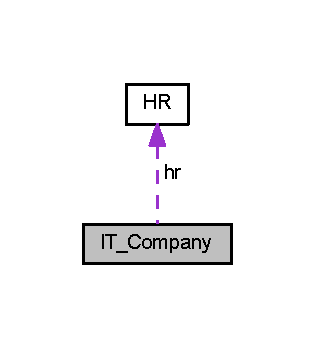
\includegraphics[width=151pt]{class_i_t___company__coll__graph}
\end{center}
\end{figure}
\subsection*{Public Member Functions}
\begin{DoxyCompactItemize}
\item 
\hyperlink{class_i_t___company_a13bea9468214205bd5b4b57c6174de9a}{I\+T\+\_\+\+Company} ()
\begin{DoxyCompactList}\small\item\em Default constructor. \end{DoxyCompactList}\item 
\hyperlink{class_i_t___company_aacbb3e9ae0d6d8a41a25785484cfc05f}{$\sim$\+I\+T\+\_\+\+Company} ()
\begin{DoxyCompactList}\small\item\em Destructor. \end{DoxyCompactList}\item 
int \hyperlink{class_i_t___company_a2753c0f3da2fb8aee6a48b3ebe3bef79}{Recruit\+People} (void)
\begin{DoxyCompactList}\small\item\em Recruit people. \end{DoxyCompactList}\item 
void \hyperlink{class_i_t___company_a652c409e38a609c96e788be7687ab744}{Set\+Name\+Of\+Company} (string v\+\_\+\+Name\+Of\+Company)
\item 
void \hyperlink{class_i_t___company_a918bdfd512ef8267cf082a20e86a63e9}{Set\+Amountof\+Employees} (int v\+\_\+\+Amountof\+Employees)
\item 
string \hyperlink{class_i_t___company_addd5ab4a8699d8df60fd2cd00a4f9875}{Get\+Name\+Of\+Company} ()
\item 
int \hyperlink{class_i_t___company_ad5210ab4e6ef0a7c9b218678645410e4}{Get\+Amountof\+Employees} ()
\item 
bool \hyperlink{class_i_t___company_a8214142064b5b8f6fed854b45f83a2aa}{Check\+Amountof\+Employees} (int v\+\_\+\+Amountof\+Employees)
\end{DoxyCompactItemize}
\subsection*{Public Attributes}
\begin{DoxyCompactItemize}
\item 
\hyperlink{class_h_r}{HR} \hyperlink{class_i_t___company_a9ef1fdbdfe9220c9f91fee83bfe65c29}{hr}
\begin{DoxyCompactList}\small\item\em Contains \hyperlink{class_h_r}{HR}. \end{DoxyCompactList}\end{DoxyCompactItemize}
\subsection*{Private Member Functions}
\begin{DoxyCompactItemize}
\item 
int \hyperlink{class_i_t___company_a06d2d0d74d96533e474618fb92291c04}{I\+T\+\_\+\+Utility} ()
\begin{DoxyCompactList}\small\item\em Utility function. \end{DoxyCompactList}\end{DoxyCompactItemize}
\subsection*{Private Attributes}
\begin{DoxyCompactItemize}
\item 
vector$<$ \hyperlink{class_employee}{Employee} $>$ \hyperlink{class_i_t___company_a26c2bb58e3f36ccc1fcfeebe651a29d2}{employee}
\begin{DoxyCompactList}\small\item\em Contains Employees. \end{DoxyCompactList}\item 
string \hyperlink{class_i_t___company_a2c19371df703f0aa969aaf8bfba32874}{Name\+Of\+Company}
\begin{DoxyCompactList}\small\item\em Contains Company Name. \end{DoxyCompactList}\item 
int \hyperlink{class_i_t___company_a5a839f7995a47589d983fd1990c06a0a}{Amountof\+Employees}
\begin{DoxyCompactList}\small\item\em Contains number of employees. \end{DoxyCompactList}\end{DoxyCompactItemize}


\subsection{Detailed Description}
I\+T\+Company class. 

Definition at line 16 of file I\+T\+\_\+\+Company.\+h.



\subsection{Constructor \& Destructor Documentation}
\mbox{\Hypertarget{class_i_t___company_a13bea9468214205bd5b4b57c6174de9a}\label{class_i_t___company_a13bea9468214205bd5b4b57c6174de9a}} 
\index{I\+T\+\_\+\+Company@{I\+T\+\_\+\+Company}!I\+T\+\_\+\+Company@{I\+T\+\_\+\+Company}}
\index{I\+T\+\_\+\+Company@{I\+T\+\_\+\+Company}!I\+T\+\_\+\+Company@{I\+T\+\_\+\+Company}}
\subsubsection{\texorpdfstring{I\+T\+\_\+\+Company()}{IT\_Company()}}
{\footnotesize\ttfamily I\+T\+\_\+\+Company\+::\+I\+T\+\_\+\+Company (\begin{DoxyParamCaption}{ }\end{DoxyParamCaption})}



Default constructor. 



Definition at line 7 of file I\+T\+\_\+\+Company.\+cpp.

\mbox{\Hypertarget{class_i_t___company_aacbb3e9ae0d6d8a41a25785484cfc05f}\label{class_i_t___company_aacbb3e9ae0d6d8a41a25785484cfc05f}} 
\index{I\+T\+\_\+\+Company@{I\+T\+\_\+\+Company}!````~I\+T\+\_\+\+Company@{$\sim$\+I\+T\+\_\+\+Company}}
\index{````~I\+T\+\_\+\+Company@{$\sim$\+I\+T\+\_\+\+Company}!I\+T\+\_\+\+Company@{I\+T\+\_\+\+Company}}
\subsubsection{\texorpdfstring{$\sim$\+I\+T\+\_\+\+Company()}{~IT\_Company()}}
{\footnotesize\ttfamily I\+T\+\_\+\+Company\+::$\sim$\+I\+T\+\_\+\+Company (\begin{DoxyParamCaption}{ }\end{DoxyParamCaption})}



Destructor. 



Definition at line 14 of file I\+T\+\_\+\+Company.\+cpp.



\subsection{Member Function Documentation}
\mbox{\Hypertarget{class_i_t___company_a8214142064b5b8f6fed854b45f83a2aa}\label{class_i_t___company_a8214142064b5b8f6fed854b45f83a2aa}} 
\index{I\+T\+\_\+\+Company@{I\+T\+\_\+\+Company}!Check\+Amountof\+Employees@{Check\+Amountof\+Employees}}
\index{Check\+Amountof\+Employees@{Check\+Amountof\+Employees}!I\+T\+\_\+\+Company@{I\+T\+\_\+\+Company}}
\subsubsection{\texorpdfstring{Check\+Amountof\+Employees()}{CheckAmountofEmployees()}}
{\footnotesize\ttfamily bool I\+T\+\_\+\+Company\+::\+Check\+Amountof\+Employees (\begin{DoxyParamCaption}\item[{int}]{v\+\_\+\+Amountof\+Employees }\end{DoxyParamCaption})}



Definition at line 116 of file I\+T\+\_\+\+Company.\+cpp.

Here is the caller graph for this function\+:
\nopagebreak
\begin{figure}[H]
\begin{center}
\leavevmode
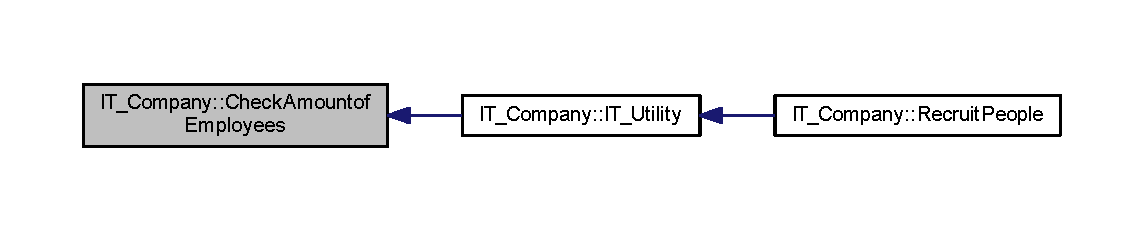
\includegraphics[width=350pt]{class_i_t___company_a8214142064b5b8f6fed854b45f83a2aa_icgraph}
\end{center}
\end{figure}
\mbox{\Hypertarget{class_i_t___company_ad5210ab4e6ef0a7c9b218678645410e4}\label{class_i_t___company_ad5210ab4e6ef0a7c9b218678645410e4}} 
\index{I\+T\+\_\+\+Company@{I\+T\+\_\+\+Company}!Get\+Amountof\+Employees@{Get\+Amountof\+Employees}}
\index{Get\+Amountof\+Employees@{Get\+Amountof\+Employees}!I\+T\+\_\+\+Company@{I\+T\+\_\+\+Company}}
\subsubsection{\texorpdfstring{Get\+Amountof\+Employees()}{GetAmountofEmployees()}}
{\footnotesize\ttfamily int I\+T\+\_\+\+Company\+::\+Get\+Amountof\+Employees (\begin{DoxyParamCaption}{ }\end{DoxyParamCaption})}



Definition at line 112 of file I\+T\+\_\+\+Company.\+cpp.

Here is the caller graph for this function\+:
\nopagebreak
\begin{figure}[H]
\begin{center}
\leavevmode
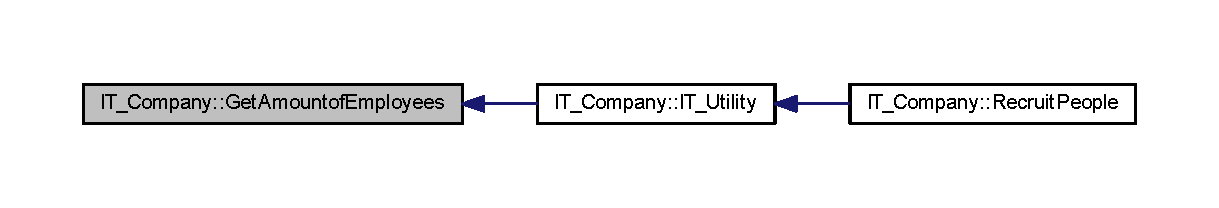
\includegraphics[width=350pt]{class_i_t___company_ad5210ab4e6ef0a7c9b218678645410e4_icgraph}
\end{center}
\end{figure}
\mbox{\Hypertarget{class_i_t___company_addd5ab4a8699d8df60fd2cd00a4f9875}\label{class_i_t___company_addd5ab4a8699d8df60fd2cd00a4f9875}} 
\index{I\+T\+\_\+\+Company@{I\+T\+\_\+\+Company}!Get\+Name\+Of\+Company@{Get\+Name\+Of\+Company}}
\index{Get\+Name\+Of\+Company@{Get\+Name\+Of\+Company}!I\+T\+\_\+\+Company@{I\+T\+\_\+\+Company}}
\subsubsection{\texorpdfstring{Get\+Name\+Of\+Company()}{GetNameOfCompany()}}
{\footnotesize\ttfamily string I\+T\+\_\+\+Company\+::\+Get\+Name\+Of\+Company (\begin{DoxyParamCaption}{ }\end{DoxyParamCaption})}



Definition at line 108 of file I\+T\+\_\+\+Company.\+cpp.

Here is the caller graph for this function\+:
\nopagebreak
\begin{figure}[H]
\begin{center}
\leavevmode
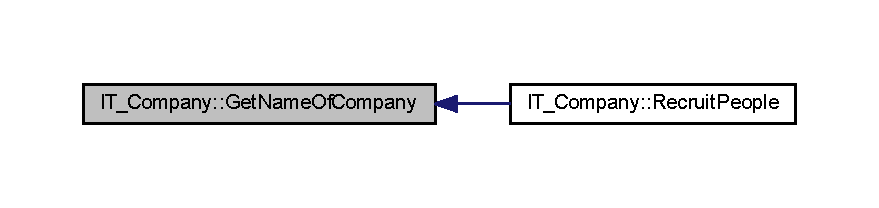
\includegraphics[width=350pt]{class_i_t___company_addd5ab4a8699d8df60fd2cd00a4f9875_icgraph}
\end{center}
\end{figure}
\mbox{\Hypertarget{class_i_t___company_a06d2d0d74d96533e474618fb92291c04}\label{class_i_t___company_a06d2d0d74d96533e474618fb92291c04}} 
\index{I\+T\+\_\+\+Company@{I\+T\+\_\+\+Company}!I\+T\+\_\+\+Utility@{I\+T\+\_\+\+Utility}}
\index{I\+T\+\_\+\+Utility@{I\+T\+\_\+\+Utility}!I\+T\+\_\+\+Company@{I\+T\+\_\+\+Company}}
\subsubsection{\texorpdfstring{I\+T\+\_\+\+Utility()}{IT\_Utility()}}
{\footnotesize\ttfamily int I\+T\+\_\+\+Company\+::\+I\+T\+\_\+\+Utility (\begin{DoxyParamCaption}{ }\end{DoxyParamCaption})\hspace{0.3cm}{\ttfamily [private]}}



Utility function. 



Definition at line 18 of file I\+T\+\_\+\+Company.\+cpp.

Here is the call graph for this function\+:
\nopagebreak
\begin{figure}[H]
\begin{center}
\leavevmode
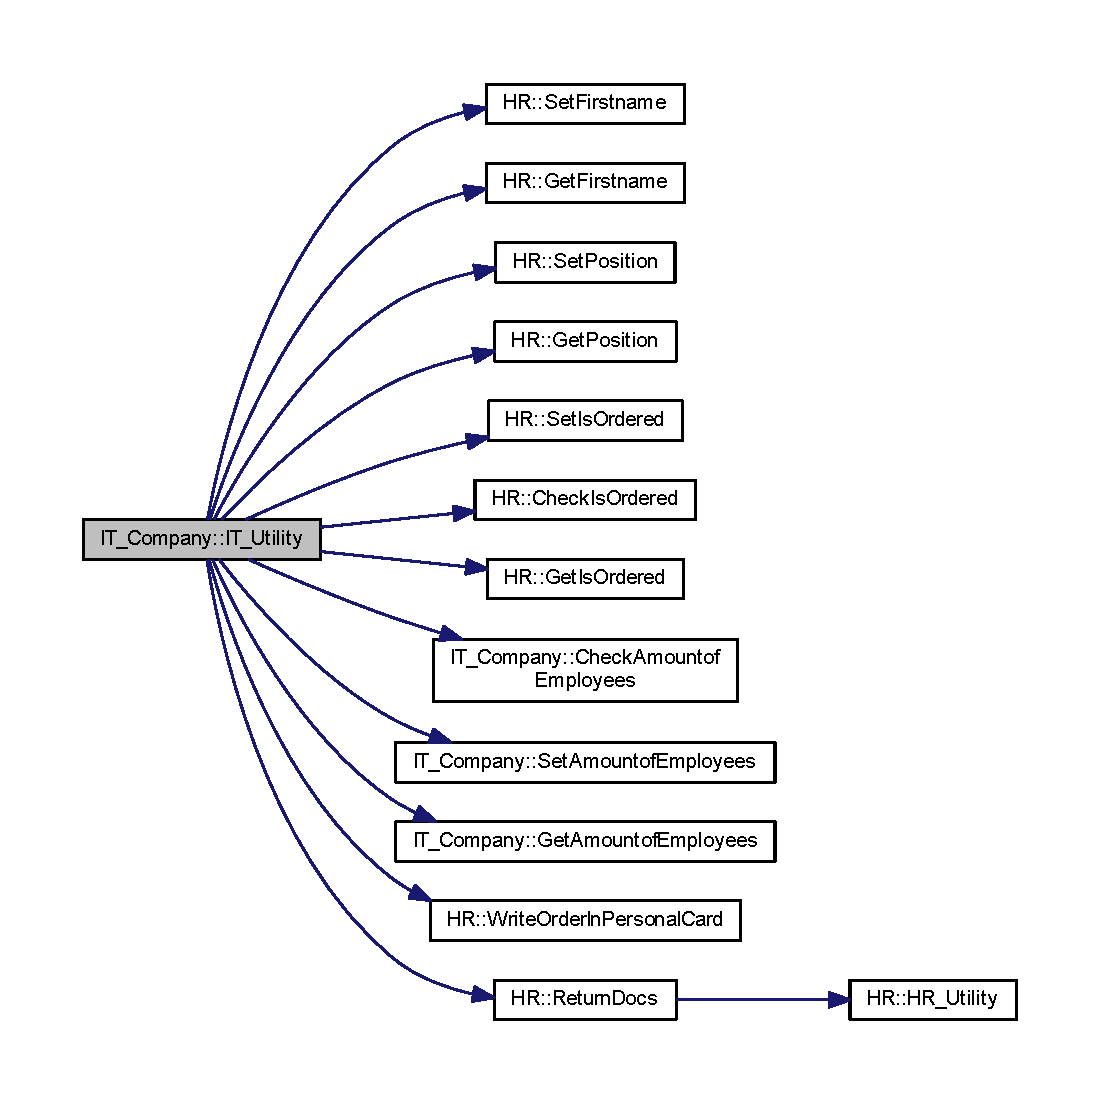
\includegraphics[width=350pt]{class_i_t___company_a06d2d0d74d96533e474618fb92291c04_cgraph}
\end{center}
\end{figure}
Here is the caller graph for this function\+:
\nopagebreak
\begin{figure}[H]
\begin{center}
\leavevmode
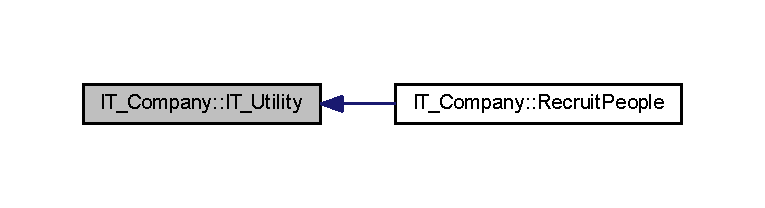
\includegraphics[width=350pt]{class_i_t___company_a06d2d0d74d96533e474618fb92291c04_icgraph}
\end{center}
\end{figure}
\mbox{\Hypertarget{class_i_t___company_a2753c0f3da2fb8aee6a48b3ebe3bef79}\label{class_i_t___company_a2753c0f3da2fb8aee6a48b3ebe3bef79}} 
\index{I\+T\+\_\+\+Company@{I\+T\+\_\+\+Company}!Recruit\+People@{Recruit\+People}}
\index{Recruit\+People@{Recruit\+People}!I\+T\+\_\+\+Company@{I\+T\+\_\+\+Company}}
\subsubsection{\texorpdfstring{Recruit\+People()}{RecruitPeople()}}
{\footnotesize\ttfamily int I\+T\+\_\+\+Company\+::\+Recruit\+People (\begin{DoxyParamCaption}\item[{void}]{ }\end{DoxyParamCaption})}



Recruit people. 



Definition at line 87 of file I\+T\+\_\+\+Company.\+cpp.

Here is the call graph for this function\+:
\nopagebreak
\begin{figure}[H]
\begin{center}
\leavevmode
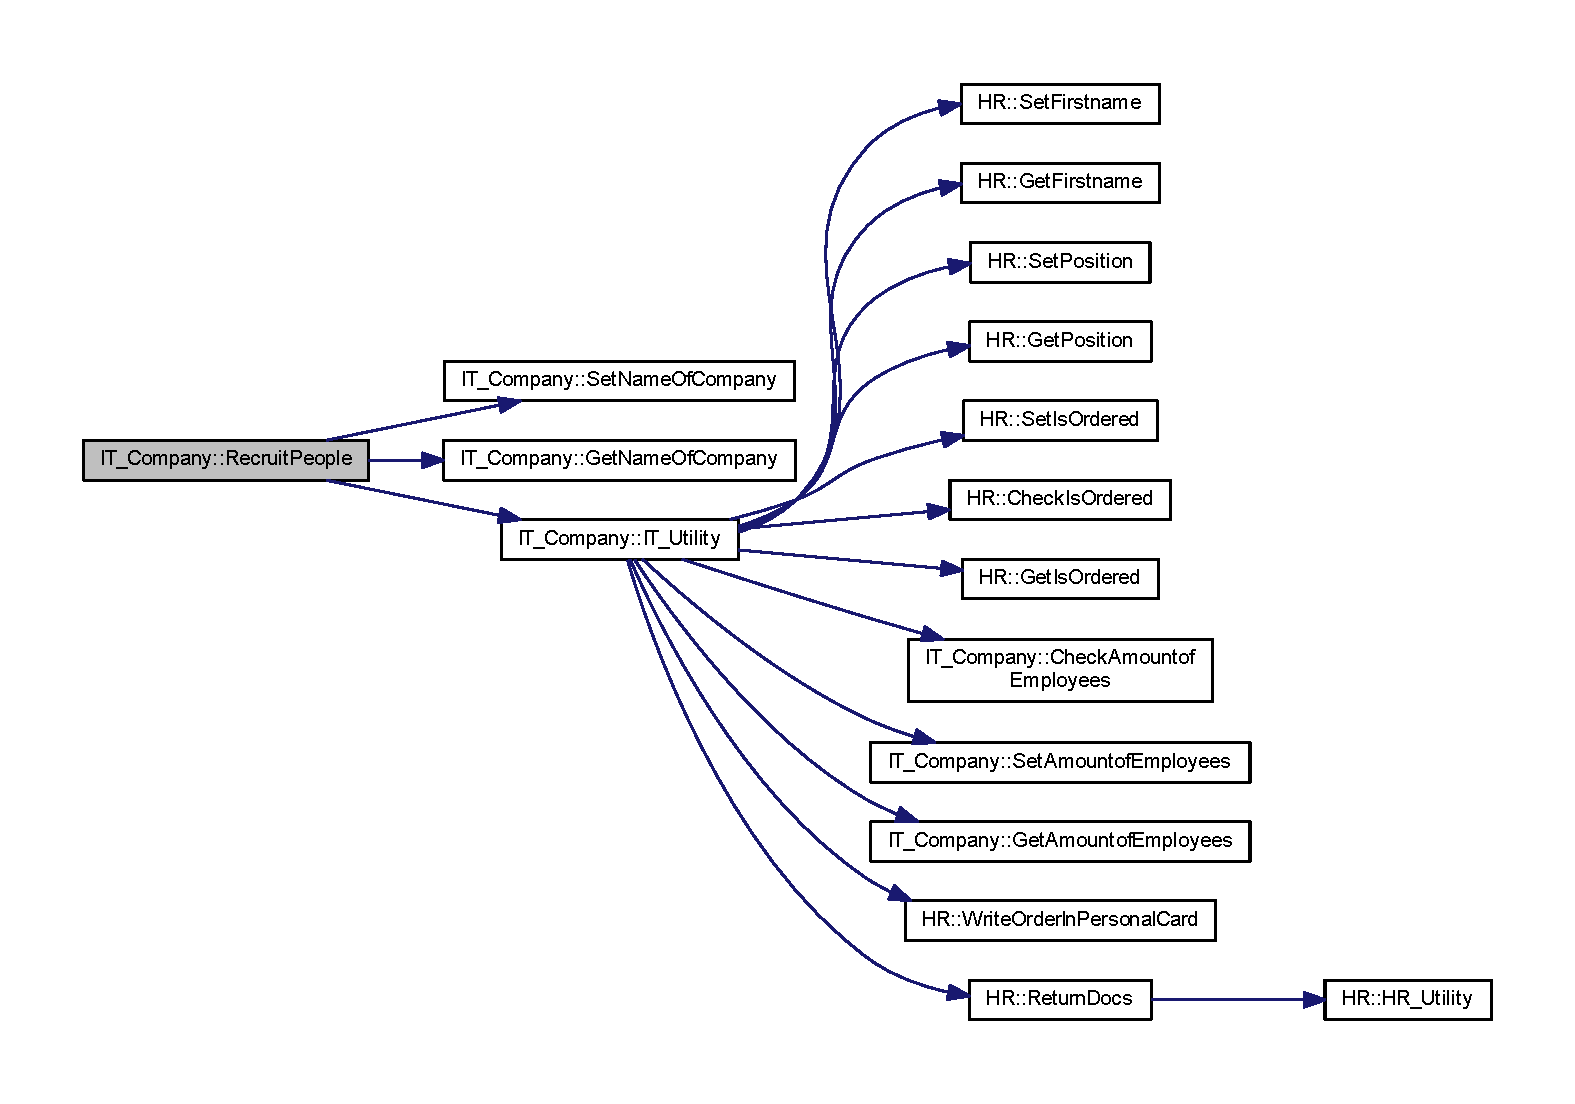
\includegraphics[width=350pt]{class_i_t___company_a2753c0f3da2fb8aee6a48b3ebe3bef79_cgraph}
\end{center}
\end{figure}
\mbox{\Hypertarget{class_i_t___company_a918bdfd512ef8267cf082a20e86a63e9}\label{class_i_t___company_a918bdfd512ef8267cf082a20e86a63e9}} 
\index{I\+T\+\_\+\+Company@{I\+T\+\_\+\+Company}!Set\+Amountof\+Employees@{Set\+Amountof\+Employees}}
\index{Set\+Amountof\+Employees@{Set\+Amountof\+Employees}!I\+T\+\_\+\+Company@{I\+T\+\_\+\+Company}}
\subsubsection{\texorpdfstring{Set\+Amountof\+Employees()}{SetAmountofEmployees()}}
{\footnotesize\ttfamily void I\+T\+\_\+\+Company\+::\+Set\+Amountof\+Employees (\begin{DoxyParamCaption}\item[{int}]{v\+\_\+\+Amountof\+Employees }\end{DoxyParamCaption})}



Definition at line 104 of file I\+T\+\_\+\+Company.\+cpp.

Here is the caller graph for this function\+:
\nopagebreak
\begin{figure}[H]
\begin{center}
\leavevmode
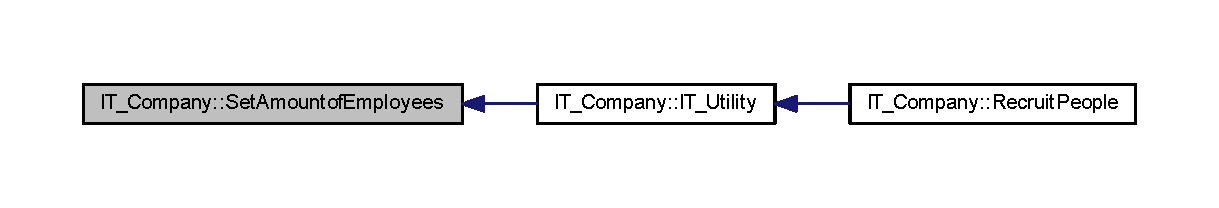
\includegraphics[width=350pt]{class_i_t___company_a918bdfd512ef8267cf082a20e86a63e9_icgraph}
\end{center}
\end{figure}
\mbox{\Hypertarget{class_i_t___company_a652c409e38a609c96e788be7687ab744}\label{class_i_t___company_a652c409e38a609c96e788be7687ab744}} 
\index{I\+T\+\_\+\+Company@{I\+T\+\_\+\+Company}!Set\+Name\+Of\+Company@{Set\+Name\+Of\+Company}}
\index{Set\+Name\+Of\+Company@{Set\+Name\+Of\+Company}!I\+T\+\_\+\+Company@{I\+T\+\_\+\+Company}}
\subsubsection{\texorpdfstring{Set\+Name\+Of\+Company()}{SetNameOfCompany()}}
{\footnotesize\ttfamily void I\+T\+\_\+\+Company\+::\+Set\+Name\+Of\+Company (\begin{DoxyParamCaption}\item[{string}]{v\+\_\+\+Name\+Of\+Company }\end{DoxyParamCaption})}



Definition at line 100 of file I\+T\+\_\+\+Company.\+cpp.

Here is the caller graph for this function\+:
\nopagebreak
\begin{figure}[H]
\begin{center}
\leavevmode
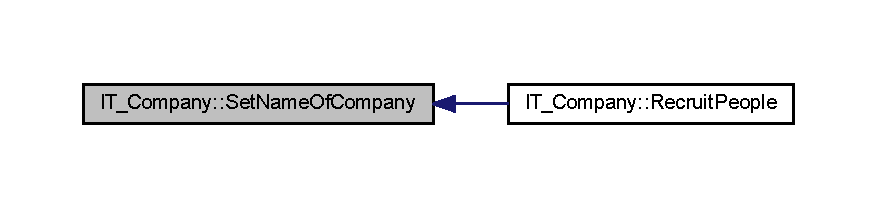
\includegraphics[width=350pt]{class_i_t___company_a652c409e38a609c96e788be7687ab744_icgraph}
\end{center}
\end{figure}


\subsection{Member Data Documentation}
\mbox{\Hypertarget{class_i_t___company_a5a839f7995a47589d983fd1990c06a0a}\label{class_i_t___company_a5a839f7995a47589d983fd1990c06a0a}} 
\index{I\+T\+\_\+\+Company@{I\+T\+\_\+\+Company}!Amountof\+Employees@{Amountof\+Employees}}
\index{Amountof\+Employees@{Amountof\+Employees}!I\+T\+\_\+\+Company@{I\+T\+\_\+\+Company}}
\subsubsection{\texorpdfstring{Amountof\+Employees}{AmountofEmployees}}
{\footnotesize\ttfamily int I\+T\+\_\+\+Company\+::\+Amountof\+Employees\hspace{0.3cm}{\ttfamily [private]}}



Contains number of employees. 



Definition at line 42 of file I\+T\+\_\+\+Company.\+h.

\mbox{\Hypertarget{class_i_t___company_a26c2bb58e3f36ccc1fcfeebe651a29d2}\label{class_i_t___company_a26c2bb58e3f36ccc1fcfeebe651a29d2}} 
\index{I\+T\+\_\+\+Company@{I\+T\+\_\+\+Company}!employee@{employee}}
\index{employee@{employee}!I\+T\+\_\+\+Company@{I\+T\+\_\+\+Company}}
\subsubsection{\texorpdfstring{employee}{employee}}
{\footnotesize\ttfamily vector$<$\hyperlink{class_employee}{Employee}$>$ I\+T\+\_\+\+Company\+::employee\hspace{0.3cm}{\ttfamily [private]}}



Contains Employees. 



Definition at line 38 of file I\+T\+\_\+\+Company.\+h.

\mbox{\Hypertarget{class_i_t___company_a9ef1fdbdfe9220c9f91fee83bfe65c29}\label{class_i_t___company_a9ef1fdbdfe9220c9f91fee83bfe65c29}} 
\index{I\+T\+\_\+\+Company@{I\+T\+\_\+\+Company}!hr@{hr}}
\index{hr@{hr}!I\+T\+\_\+\+Company@{I\+T\+\_\+\+Company}}
\subsubsection{\texorpdfstring{hr}{hr}}
{\footnotesize\ttfamily \hyperlink{class_h_r}{HR} I\+T\+\_\+\+Company\+::hr}



Contains \hyperlink{class_h_r}{HR}. 



Definition at line 28 of file I\+T\+\_\+\+Company.\+h.

\mbox{\Hypertarget{class_i_t___company_a2c19371df703f0aa969aaf8bfba32874}\label{class_i_t___company_a2c19371df703f0aa969aaf8bfba32874}} 
\index{I\+T\+\_\+\+Company@{I\+T\+\_\+\+Company}!Name\+Of\+Company@{Name\+Of\+Company}}
\index{Name\+Of\+Company@{Name\+Of\+Company}!I\+T\+\_\+\+Company@{I\+T\+\_\+\+Company}}
\subsubsection{\texorpdfstring{Name\+Of\+Company}{NameOfCompany}}
{\footnotesize\ttfamily string I\+T\+\_\+\+Company\+::\+Name\+Of\+Company\hspace{0.3cm}{\ttfamily [private]}}



Contains Company Name. 



Definition at line 40 of file I\+T\+\_\+\+Company.\+h.



The documentation for this class was generated from the following files\+:\begin{DoxyCompactItemize}
\item 
C\+:/\+Workspace/\+I\+T\+Company\+Cpp/\+I\+T\+Company/\+I\+T\+Company/\hyperlink{_i_t___company_8h}{I\+T\+\_\+\+Company.\+h}\item 
C\+:/\+Workspace/\+I\+T\+Company\+Cpp/\+I\+T\+Company/\+I\+T\+Company/\hyperlink{_i_t___company_8cpp}{I\+T\+\_\+\+Company.\+cpp}\end{DoxyCompactItemize}

\hypertarget{class_personal_card}{}\section{Personal\+Card Class Reference}
\label{class_personal_card}\index{Personal\+Card@{Personal\+Card}}


\hyperlink{class_personal_card}{Personal\+Card} class.  




{\ttfamily \#include $<$Personal\+Card.\+h$>$}

\subsection*{Public Member Functions}
\begin{DoxyCompactItemize}
\item 
\hyperlink{class_personal_card_aacffa8a4bdb2d9f94456f40ca4ed13fd}{Personal\+Card} ()
\item 
\hyperlink{class_personal_card_af091bd8305d36b1c8766a1f229f39e8e}{$\sim$\+Personal\+Card} ()
\begin{DoxyCompactList}\small\item\em Destructor. \end{DoxyCompactList}\item 
string \hyperlink{class_personal_card_a774f3b78adef43c85249fe79b3033d38}{Create} (void)
\item 
void \hyperlink{class_personal_card_a16bfc51a2799441fd51dc5a9629aaf84}{Set\+First\+Name} (string v\+\_\+\+First\+Name)
\item 
void \hyperlink{class_personal_card_a4e730d56dc6b1ceb02caaa5f7bd22355}{Set\+Mark\+In\+Employment\+History\+Book} (string v\+\_\+\+Mark\+In\+Employment\+History\+Book)
\item 
void \hyperlink{class_personal_card_a16506f3197fea963fc3b2d0adfd66cc4}{Set\+Birthday} (string v\+\_\+\+Birthday)
\item 
void \hyperlink{class_personal_card_a764a8481bcb8dcef50e9cb8c6494d57f}{Set\+Birthday\+Place} (string v\+\_\+\+Birthday\+Place)
\item 
void \hyperlink{class_personal_card_a48115ca8e0f475555b54d433c2afc520}{Set\+Current\+Experience} (int v\+\_\+\+Current\+Experience)
\item 
void \hyperlink{class_personal_card_a29fa16d9f23752ed9a816deaba9cbddc}{Set\+Position} (string v\+\_\+\+Position)
\item 
void \hyperlink{class_personal_card_a965fb1e37dade935ea62d0c520559acf}{Set\+Pension\+Certificate} (string v\+\_\+\+Pension\+Certificate)
\item 
void \hyperlink{class_personal_card_a2e9ddff06c5ff0e22949d24505f40ccd}{Set\+Medical\+Insurance} (string v\+\_\+\+Medical\+Insurance)
\item 
void \hyperlink{class_personal_card_a8bb3282bbfb14220af810833040b6b54}{Set\+Tax\+ID} (string v\+\_\+\+Tax\+ID)
\item 
void \hyperlink{class_personal_card_ac1afd2dd3136a2309be0176aa66dbf80}{Set\+Marital\+Status} (string v\+\_\+\+Marital\+Status)
\item 
void \hyperlink{class_personal_card_a7d69b0978b5fb6ea6e73845bbb2bbb9f}{Set\+Children} (int v\+\_\+\+Children)
\item 
void \hyperlink{class_personal_card_a77e6093986bbc85c7e3c059e5917f644}{Set\+Education\+Document} (string v\+\_\+\+Education\+Document)
\item 
void \hyperlink{class_personal_card_a3ca640fa4e9a91c78c02b7c9cc54d3fc}{Set\+Passport\+Numberand\+Series} (string v\+\_\+\+Passport\+Numberand\+Series)
\item 
string \hyperlink{class_personal_card_a19b7a8415b6884ae8b3bf7ae0d87b7ba}{Get\+First\+Name} ()
\item 
string \hyperlink{class_personal_card_a997c73c07747e9827a9ceb7485f80641}{Get\+Mark\+In\+Employment\+History\+Book} ()
\item 
string \hyperlink{class_personal_card_a11047dcaa640d5170477318e5baef1e5}{Get\+Birhday} ()
\item 
string \hyperlink{class_personal_card_ad859469f1bd01abd223a0e2a022c41ba}{Get\+Birthday\+Place} ()
\item 
int \hyperlink{class_personal_card_afd7705ca4f1900df16fc24a9ed60b0b1}{Get\+Current\+Experience} ()
\item 
string \hyperlink{class_personal_card_a29f5b5c9afad6d7ff3d9d0eb97f7d8ea}{Get\+Position} ()
\item 
string \hyperlink{class_personal_card_ab73d926e143e0771ca4af7f06e4c1c4e}{Get\+Pension\+Certificate} ()
\item 
string \hyperlink{class_personal_card_a26846e9e2d225d7db37cca1831eca69c}{Get\+Medical\+Insurance} ()
\item 
string \hyperlink{class_personal_card_a51916b1375d50c9c914fa5e49b59d653}{Get\+Tax\+ID} ()
\item 
string \hyperlink{class_personal_card_a0732cc495fb1208c9b46d7dd72c6d261}{Get\+Marital\+Status} ()
\item 
int \hyperlink{class_personal_card_af2d6c90909a49f8fb8dabf2ec5d1bd96}{Get\+Children} ()
\item 
string \hyperlink{class_personal_card_a603ff1ccfda3befb27426a1416640faa}{Get\+Education\+Document} ()
\item 
string \hyperlink{class_personal_card_a8ecd57bcbfac1f95f14aabbdb71d418c}{Get\+Passport\+Numberand\+Series} ()
\item 
bool \hyperlink{class_personal_card_a9a6e00618504841576370a6f33d5a3ea}{Check\+Current\+Experience} (int �urrent\+Experience)
\item 
bool \hyperlink{class_personal_card_a5e5249e91b615c70b6f8dfed3757ffe7}{Check\+Children} (int �hildren)
\end{DoxyCompactItemize}
\subsection*{Private Member Functions}
\begin{DoxyCompactItemize}
\item 
void \hyperlink{class_personal_card_a6a77263e418dd177303bbc03b78256c2}{P\+C\+\_\+\+Utility} ()
\begin{DoxyCompactList}\small\item\em Utility funxtion. \end{DoxyCompactList}\end{DoxyCompactItemize}
\subsection*{Private Attributes}
\begin{DoxyCompactItemize}
\item 
string \hyperlink{class_personal_card_a5d886372e6fd85fd201dd7197858b87f}{First\+Name}
\begin{DoxyCompactList}\small\item\em firstname \end{DoxyCompactList}\item 
string \hyperlink{class_personal_card_aca45730500482ce9cabb9cb867221bfe}{Mark\+In\+Employment\+History\+Book}
\begin{DoxyCompactList}\small\item\em Mark\+In\+Employment\+History\+Book. \end{DoxyCompactList}\item 
string \hyperlink{class_personal_card_a66f3010ea772ee8f4558366511195caa}{Birthday}
\begin{DoxyCompactList}\small\item\em Birthday. \end{DoxyCompactList}\item 
string \hyperlink{class_personal_card_a7804218412178d0e188ae084effca73c}{Birthday\+Place}
\begin{DoxyCompactList}\small\item\em Birthday\+Place. \end{DoxyCompactList}\item 
int \hyperlink{class_personal_card_a5629b515000706a5d4d0b6b981e2d258}{Current\+Experience}
\begin{DoxyCompactList}\small\item\em Current\+Experience. \end{DoxyCompactList}\item 
string \hyperlink{class_personal_card_a9c2275134da8725a41855aa4050c51dc}{Position}
\begin{DoxyCompactList}\small\item\em Position. \end{DoxyCompactList}\item 
string \hyperlink{class_personal_card_a14e321878525cd3275d28e5600c34834}{Pension\+Certificate}
\begin{DoxyCompactList}\small\item\em Pension\+Certificate. \end{DoxyCompactList}\item 
string \hyperlink{class_personal_card_a4742180fadcf4f32bc3e825dddc369b3}{Medical\+Insurance}
\begin{DoxyCompactList}\small\item\em Medical\+Insurance. \end{DoxyCompactList}\item 
string \hyperlink{class_personal_card_ac24b7e68e8bde96a92fccb67a21a5254}{Tax\+ID}
\begin{DoxyCompactList}\small\item\em Tax\+ID. \end{DoxyCompactList}\item 
string \hyperlink{class_personal_card_a9e13327f59ee2b29c32feb5d3b903dcd}{Marital\+Status}
\begin{DoxyCompactList}\small\item\em Marital\+Status. \end{DoxyCompactList}\item 
int \hyperlink{class_personal_card_a4c3448e9aded5212ea510c432e49943b}{Children}
\begin{DoxyCompactList}\small\item\em Children. \end{DoxyCompactList}\item 
string \hyperlink{class_personal_card_a7f39109985c882f26e81a6ba6a3838ef}{Education\+Document}
\begin{DoxyCompactList}\small\item\em Education\+Document. \end{DoxyCompactList}\item 
string \hyperlink{class_personal_card_a25cc725250662caceff129745eeca080}{Passport\+Numberand\+Series}
\begin{DoxyCompactList}\small\item\em Passport\+Numberand\+Series. \end{DoxyCompactList}\end{DoxyCompactItemize}


\subsection{Detailed Description}
\hyperlink{class_personal_card}{Personal\+Card} class. 

Definition at line 12 of file Personal\+Card.\+h.



\subsection{Constructor \& Destructor Documentation}
\mbox{\Hypertarget{class_personal_card_aacffa8a4bdb2d9f94456f40ca4ed13fd}\label{class_personal_card_aacffa8a4bdb2d9f94456f40ca4ed13fd}} 
\index{Personal\+Card@{Personal\+Card}!Personal\+Card@{Personal\+Card}}
\index{Personal\+Card@{Personal\+Card}!Personal\+Card@{Personal\+Card}}
\subsubsection{\texorpdfstring{Personal\+Card()}{PersonalCard()}}
{\footnotesize\ttfamily Personal\+Card\+::\+Personal\+Card (\begin{DoxyParamCaption}{ }\end{DoxyParamCaption})}



Definition at line 3 of file Personal\+Card.\+cpp.

\mbox{\Hypertarget{class_personal_card_af091bd8305d36b1c8766a1f229f39e8e}\label{class_personal_card_af091bd8305d36b1c8766a1f229f39e8e}} 
\index{Personal\+Card@{Personal\+Card}!````~Personal\+Card@{$\sim$\+Personal\+Card}}
\index{````~Personal\+Card@{$\sim$\+Personal\+Card}!Personal\+Card@{Personal\+Card}}
\subsubsection{\texorpdfstring{$\sim$\+Personal\+Card()}{~PersonalCard()}}
{\footnotesize\ttfamily Personal\+Card\+::$\sim$\+Personal\+Card (\begin{DoxyParamCaption}{ }\end{DoxyParamCaption})}



Destructor. 



Definition at line 6 of file Personal\+Card.\+cpp.



\subsection{Member Function Documentation}
\mbox{\Hypertarget{class_personal_card_a5e5249e91b615c70b6f8dfed3757ffe7}\label{class_personal_card_a5e5249e91b615c70b6f8dfed3757ffe7}} 
\index{Personal\+Card@{Personal\+Card}!Check\+Children@{Check\+Children}}
\index{Check\+Children@{Check\+Children}!Personal\+Card@{Personal\+Card}}
\subsubsection{\texorpdfstring{Check\+Children()}{CheckChildren()}}
{\footnotesize\ttfamily bool Personal\+Card\+::\+Check\+Children (\begin{DoxyParamCaption}\item[{int}]{�hildren }\end{DoxyParamCaption})}



Definition at line 224 of file Personal\+Card.\+cpp.

Here is the caller graph for this function\+:
\nopagebreak
\begin{figure}[H]
\begin{center}
\leavevmode
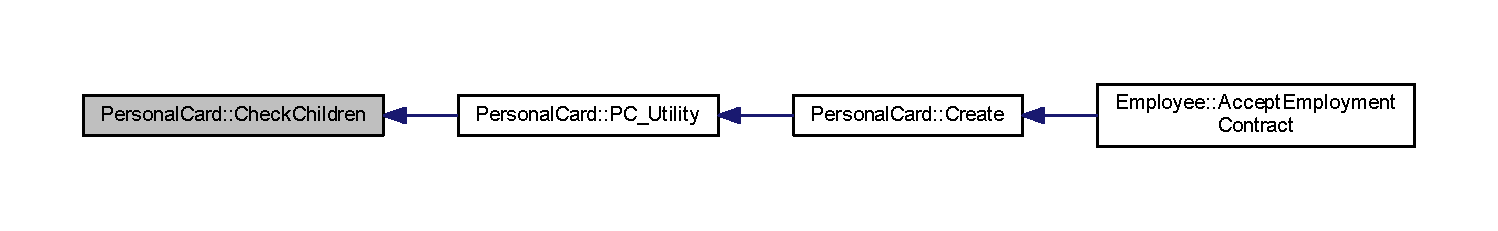
\includegraphics[width=350pt]{class_personal_card_a5e5249e91b615c70b6f8dfed3757ffe7_icgraph}
\end{center}
\end{figure}
\mbox{\Hypertarget{class_personal_card_a9a6e00618504841576370a6f33d5a3ea}\label{class_personal_card_a9a6e00618504841576370a6f33d5a3ea}} 
\index{Personal\+Card@{Personal\+Card}!Check\+Current\+Experience@{Check\+Current\+Experience}}
\index{Check\+Current\+Experience@{Check\+Current\+Experience}!Personal\+Card@{Personal\+Card}}
\subsubsection{\texorpdfstring{Check\+Current\+Experience()}{CheckCurrentExperience()}}
{\footnotesize\ttfamily bool Personal\+Card\+::\+Check\+Current\+Experience (\begin{DoxyParamCaption}\item[{int}]{�urrent\+Experience }\end{DoxyParamCaption})}



Definition at line 218 of file Personal\+Card.\+cpp.

Here is the caller graph for this function\+:
\nopagebreak
\begin{figure}[H]
\begin{center}
\leavevmode
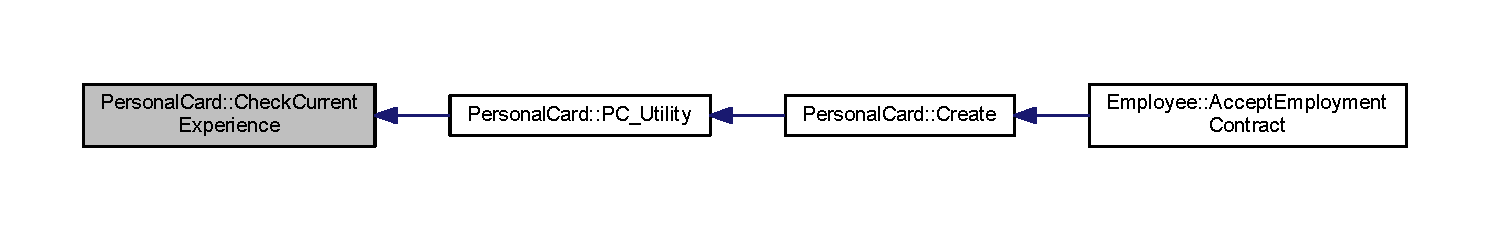
\includegraphics[width=350pt]{class_personal_card_a9a6e00618504841576370a6f33d5a3ea_icgraph}
\end{center}
\end{figure}
\mbox{\Hypertarget{class_personal_card_a774f3b78adef43c85249fe79b3033d38}\label{class_personal_card_a774f3b78adef43c85249fe79b3033d38}} 
\index{Personal\+Card@{Personal\+Card}!Create@{Create}}
\index{Create@{Create}!Personal\+Card@{Personal\+Card}}
\subsubsection{\texorpdfstring{Create()}{Create()}}
{\footnotesize\ttfamily std\+::string Personal\+Card\+::\+Create (\begin{DoxyParamCaption}\item[{void}]{ }\end{DoxyParamCaption})}



Definition at line 104 of file Personal\+Card.\+cpp.

Here is the call graph for this function\+:
\nopagebreak
\begin{figure}[H]
\begin{center}
\leavevmode
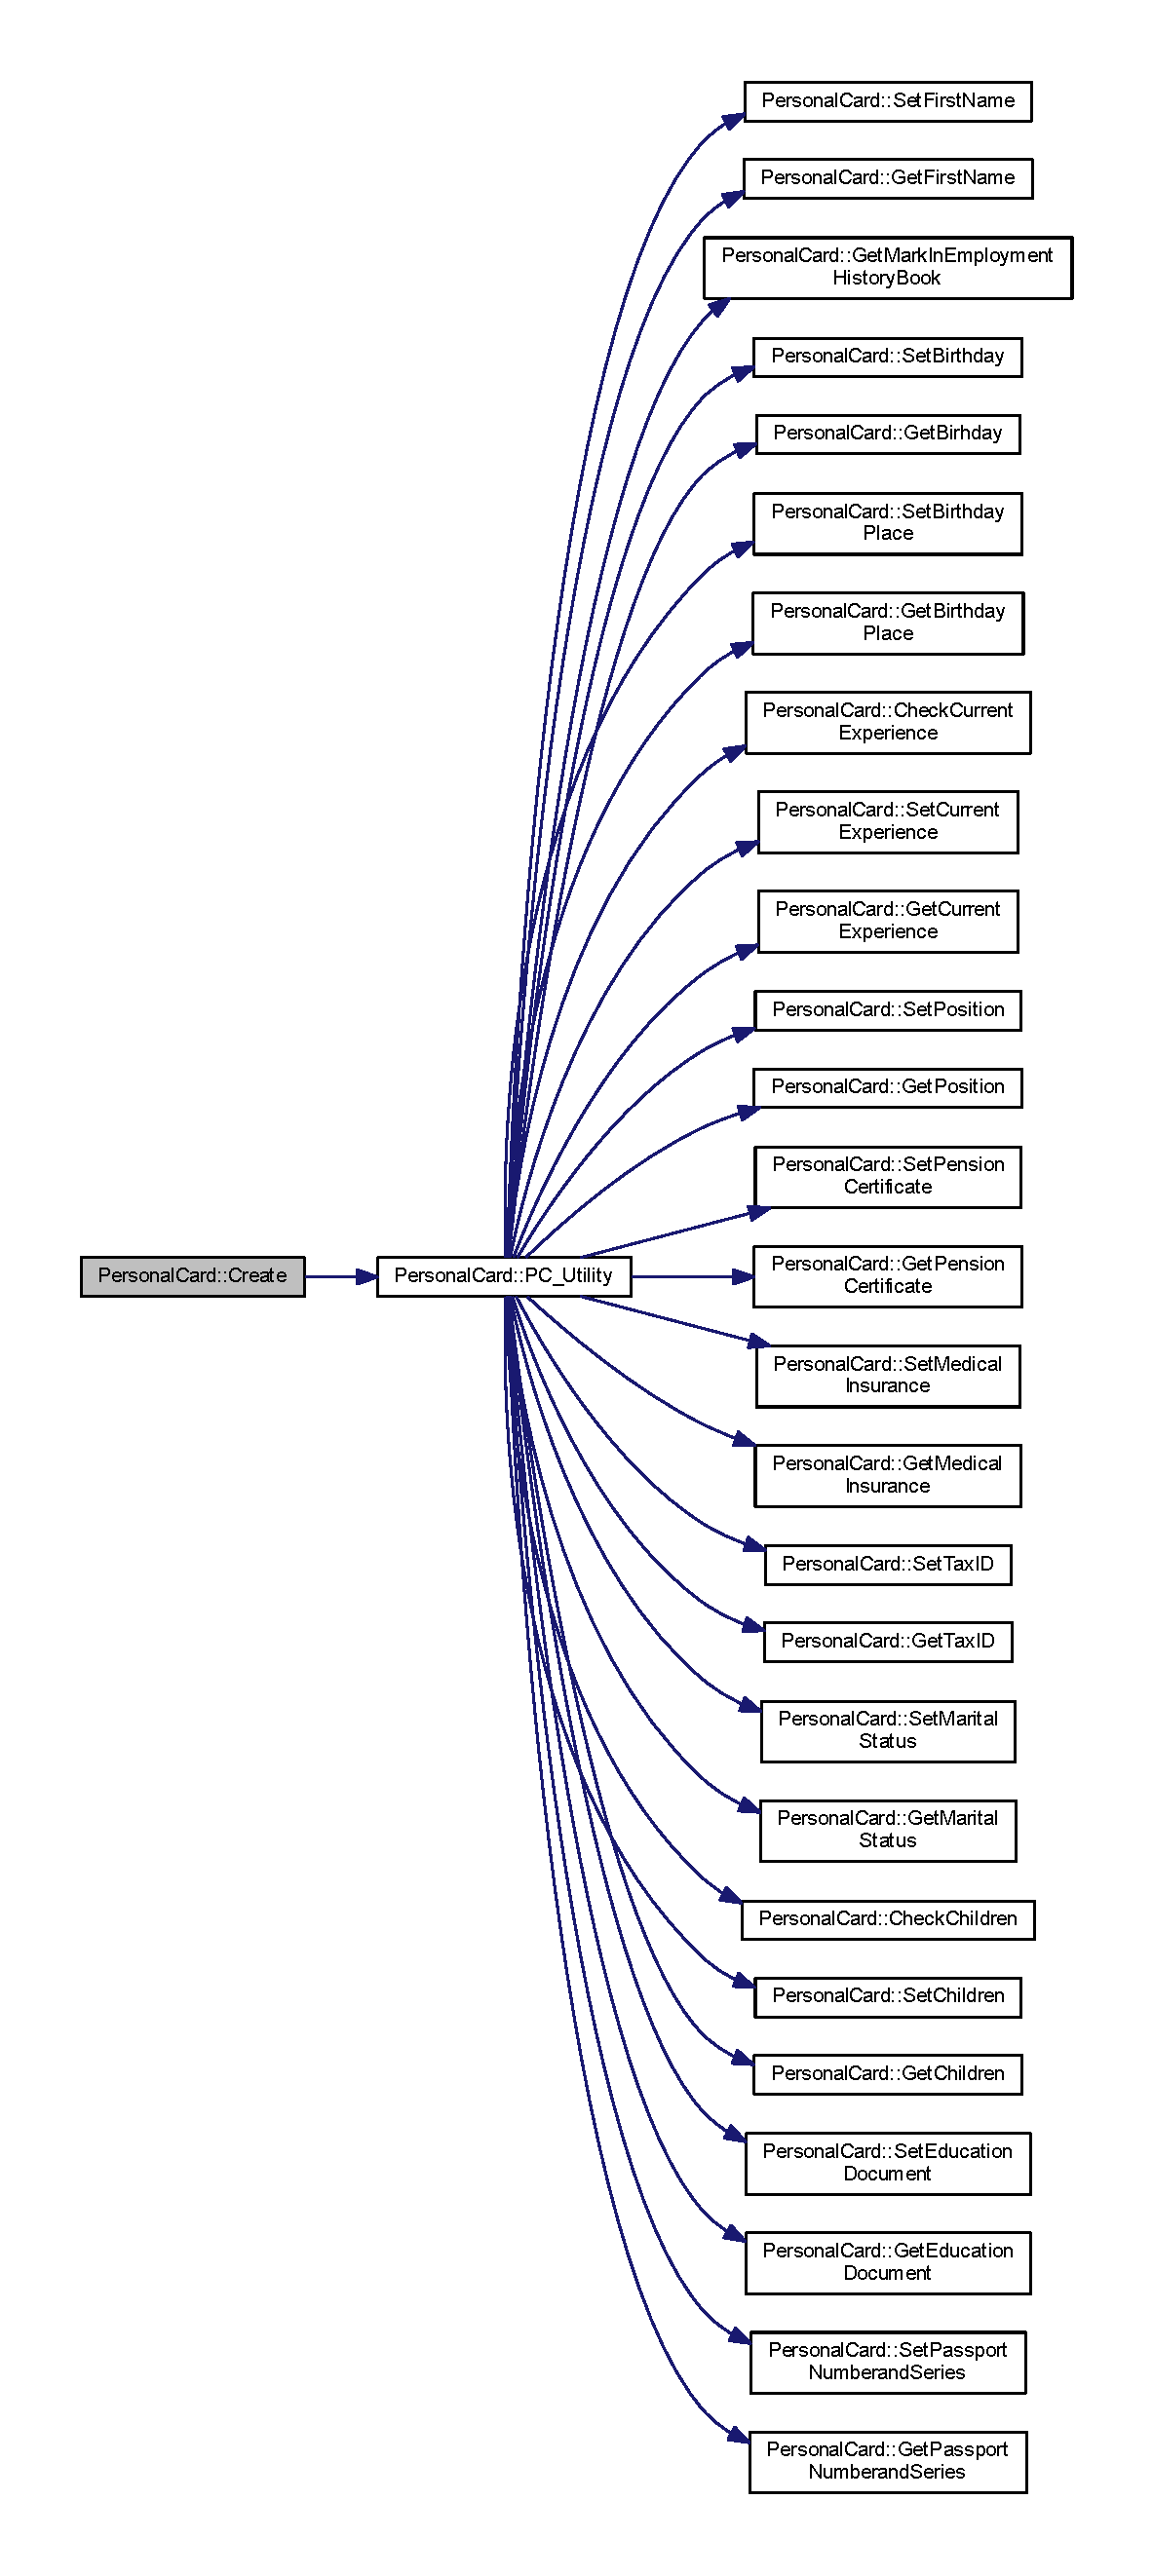
\includegraphics[height=550pt]{class_personal_card_a774f3b78adef43c85249fe79b3033d38_cgraph}
\end{center}
\end{figure}
Here is the caller graph for this function\+:
\nopagebreak
\begin{figure}[H]
\begin{center}
\leavevmode
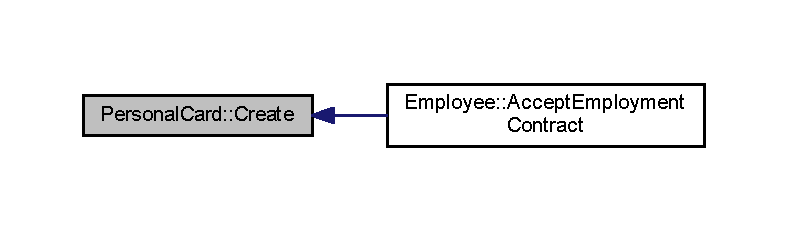
\includegraphics[width=350pt]{class_personal_card_a774f3b78adef43c85249fe79b3033d38_icgraph}
\end{center}
\end{figure}
\mbox{\Hypertarget{class_personal_card_a11047dcaa640d5170477318e5baef1e5}\label{class_personal_card_a11047dcaa640d5170477318e5baef1e5}} 
\index{Personal\+Card@{Personal\+Card}!Get\+Birhday@{Get\+Birhday}}
\index{Get\+Birhday@{Get\+Birhday}!Personal\+Card@{Personal\+Card}}
\subsubsection{\texorpdfstring{Get\+Birhday()}{GetBirhday()}}
{\footnotesize\ttfamily string Personal\+Card\+::\+Get\+Birhday (\begin{DoxyParamCaption}{ }\end{DoxyParamCaption})}



Definition at line 174 of file Personal\+Card.\+cpp.

Here is the caller graph for this function\+:
\nopagebreak
\begin{figure}[H]
\begin{center}
\leavevmode
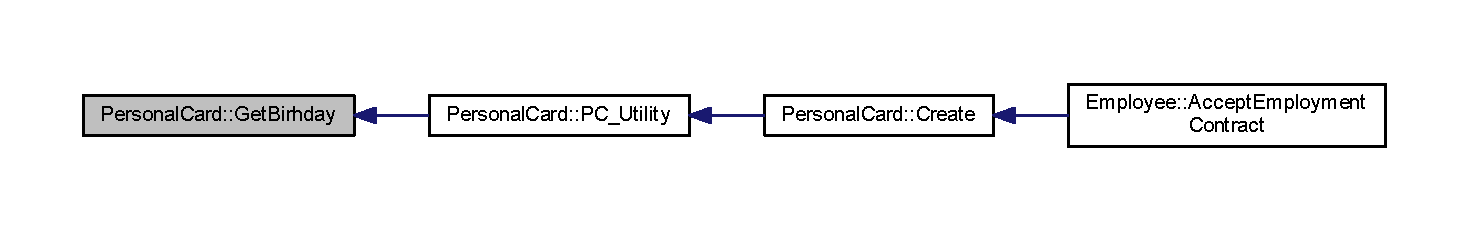
\includegraphics[width=350pt]{class_personal_card_a11047dcaa640d5170477318e5baef1e5_icgraph}
\end{center}
\end{figure}
\mbox{\Hypertarget{class_personal_card_ad859469f1bd01abd223a0e2a022c41ba}\label{class_personal_card_ad859469f1bd01abd223a0e2a022c41ba}} 
\index{Personal\+Card@{Personal\+Card}!Get\+Birthday\+Place@{Get\+Birthday\+Place}}
\index{Get\+Birthday\+Place@{Get\+Birthday\+Place}!Personal\+Card@{Personal\+Card}}
\subsubsection{\texorpdfstring{Get\+Birthday\+Place()}{GetBirthdayPlace()}}
{\footnotesize\ttfamily string Personal\+Card\+::\+Get\+Birthday\+Place (\begin{DoxyParamCaption}{ }\end{DoxyParamCaption})}



Definition at line 178 of file Personal\+Card.\+cpp.

Here is the caller graph for this function\+:
\nopagebreak
\begin{figure}[H]
\begin{center}
\leavevmode
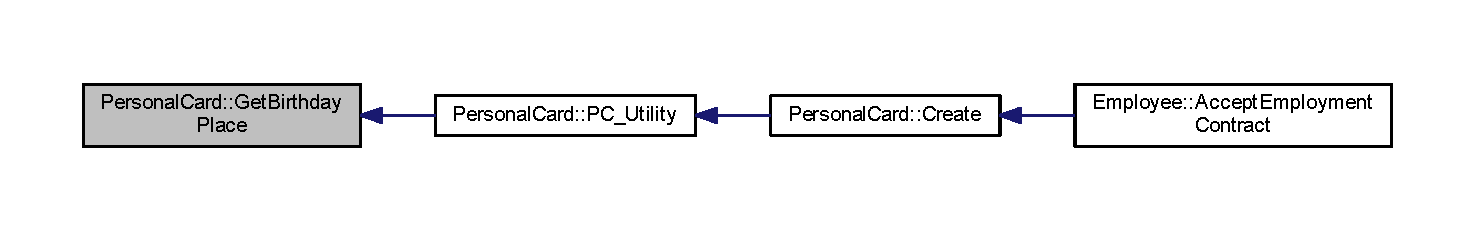
\includegraphics[width=350pt]{class_personal_card_ad859469f1bd01abd223a0e2a022c41ba_icgraph}
\end{center}
\end{figure}
\mbox{\Hypertarget{class_personal_card_af2d6c90909a49f8fb8dabf2ec5d1bd96}\label{class_personal_card_af2d6c90909a49f8fb8dabf2ec5d1bd96}} 
\index{Personal\+Card@{Personal\+Card}!Get\+Children@{Get\+Children}}
\index{Get\+Children@{Get\+Children}!Personal\+Card@{Personal\+Card}}
\subsubsection{\texorpdfstring{Get\+Children()}{GetChildren()}}
{\footnotesize\ttfamily int Personal\+Card\+::\+Get\+Children (\begin{DoxyParamCaption}{ }\end{DoxyParamCaption})}



Definition at line 206 of file Personal\+Card.\+cpp.

Here is the caller graph for this function\+:
\nopagebreak
\begin{figure}[H]
\begin{center}
\leavevmode
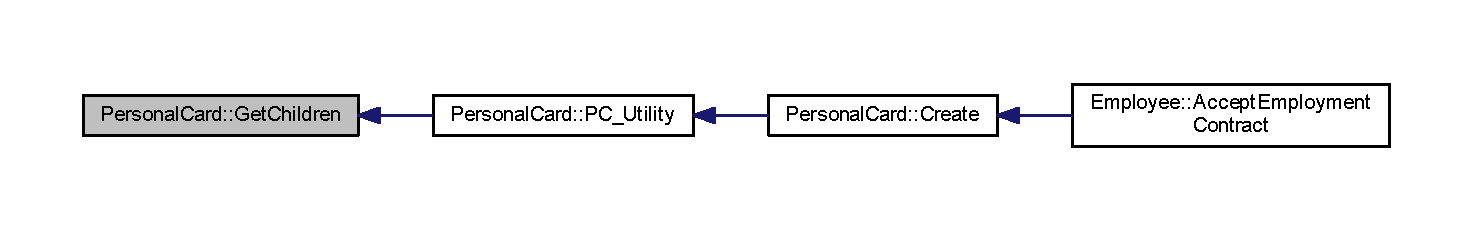
\includegraphics[width=350pt]{class_personal_card_af2d6c90909a49f8fb8dabf2ec5d1bd96_icgraph}
\end{center}
\end{figure}
\mbox{\Hypertarget{class_personal_card_afd7705ca4f1900df16fc24a9ed60b0b1}\label{class_personal_card_afd7705ca4f1900df16fc24a9ed60b0b1}} 
\index{Personal\+Card@{Personal\+Card}!Get\+Current\+Experience@{Get\+Current\+Experience}}
\index{Get\+Current\+Experience@{Get\+Current\+Experience}!Personal\+Card@{Personal\+Card}}
\subsubsection{\texorpdfstring{Get\+Current\+Experience()}{GetCurrentExperience()}}
{\footnotesize\ttfamily int Personal\+Card\+::\+Get\+Current\+Experience (\begin{DoxyParamCaption}{ }\end{DoxyParamCaption})}



Definition at line 182 of file Personal\+Card.\+cpp.

Here is the caller graph for this function\+:
\nopagebreak
\begin{figure}[H]
\begin{center}
\leavevmode
\includegraphics[width=350pt]{class_personal_card_afd7705ca4f1900df16fc24a9ed60b0b1_icgraph}
\end{center}
\end{figure}
\mbox{\Hypertarget{class_personal_card_a603ff1ccfda3befb27426a1416640faa}\label{class_personal_card_a603ff1ccfda3befb27426a1416640faa}} 
\index{Personal\+Card@{Personal\+Card}!Get\+Education\+Document@{Get\+Education\+Document}}
\index{Get\+Education\+Document@{Get\+Education\+Document}!Personal\+Card@{Personal\+Card}}
\subsubsection{\texorpdfstring{Get\+Education\+Document()}{GetEducationDocument()}}
{\footnotesize\ttfamily string Personal\+Card\+::\+Get\+Education\+Document (\begin{DoxyParamCaption}{ }\end{DoxyParamCaption})}



Definition at line 210 of file Personal\+Card.\+cpp.

Here is the caller graph for this function\+:
\nopagebreak
\begin{figure}[H]
\begin{center}
\leavevmode
\includegraphics[width=350pt]{class_personal_card_a603ff1ccfda3befb27426a1416640faa_icgraph}
\end{center}
\end{figure}
\mbox{\Hypertarget{class_personal_card_a19b7a8415b6884ae8b3bf7ae0d87b7ba}\label{class_personal_card_a19b7a8415b6884ae8b3bf7ae0d87b7ba}} 
\index{Personal\+Card@{Personal\+Card}!Get\+First\+Name@{Get\+First\+Name}}
\index{Get\+First\+Name@{Get\+First\+Name}!Personal\+Card@{Personal\+Card}}
\subsubsection{\texorpdfstring{Get\+First\+Name()}{GetFirstName()}}
{\footnotesize\ttfamily string Personal\+Card\+::\+Get\+First\+Name (\begin{DoxyParamCaption}{ }\end{DoxyParamCaption})}



Definition at line 166 of file Personal\+Card.\+cpp.

Here is the caller graph for this function\+:
\nopagebreak
\begin{figure}[H]
\begin{center}
\leavevmode
\includegraphics[width=350pt]{class_personal_card_a19b7a8415b6884ae8b3bf7ae0d87b7ba_icgraph}
\end{center}
\end{figure}
\mbox{\Hypertarget{class_personal_card_a0732cc495fb1208c9b46d7dd72c6d261}\label{class_personal_card_a0732cc495fb1208c9b46d7dd72c6d261}} 
\index{Personal\+Card@{Personal\+Card}!Get\+Marital\+Status@{Get\+Marital\+Status}}
\index{Get\+Marital\+Status@{Get\+Marital\+Status}!Personal\+Card@{Personal\+Card}}
\subsubsection{\texorpdfstring{Get\+Marital\+Status()}{GetMaritalStatus()}}
{\footnotesize\ttfamily string Personal\+Card\+::\+Get\+Marital\+Status (\begin{DoxyParamCaption}{ }\end{DoxyParamCaption})}



Definition at line 202 of file Personal\+Card.\+cpp.

Here is the caller graph for this function\+:
\nopagebreak
\begin{figure}[H]
\begin{center}
\leavevmode
\includegraphics[width=350pt]{class_personal_card_a0732cc495fb1208c9b46d7dd72c6d261_icgraph}
\end{center}
\end{figure}
\mbox{\Hypertarget{class_personal_card_a997c73c07747e9827a9ceb7485f80641}\label{class_personal_card_a997c73c07747e9827a9ceb7485f80641}} 
\index{Personal\+Card@{Personal\+Card}!Get\+Mark\+In\+Employment\+History\+Book@{Get\+Mark\+In\+Employment\+History\+Book}}
\index{Get\+Mark\+In\+Employment\+History\+Book@{Get\+Mark\+In\+Employment\+History\+Book}!Personal\+Card@{Personal\+Card}}
\subsubsection{\texorpdfstring{Get\+Mark\+In\+Employment\+History\+Book()}{GetMarkInEmploymentHistoryBook()}}
{\footnotesize\ttfamily string Personal\+Card\+::\+Get\+Mark\+In\+Employment\+History\+Book (\begin{DoxyParamCaption}{ }\end{DoxyParamCaption})}



Definition at line 170 of file Personal\+Card.\+cpp.

Here is the caller graph for this function\+:
\nopagebreak
\begin{figure}[H]
\begin{center}
\leavevmode
\includegraphics[width=350pt]{class_personal_card_a997c73c07747e9827a9ceb7485f80641_icgraph}
\end{center}
\end{figure}
\mbox{\Hypertarget{class_personal_card_a26846e9e2d225d7db37cca1831eca69c}\label{class_personal_card_a26846e9e2d225d7db37cca1831eca69c}} 
\index{Personal\+Card@{Personal\+Card}!Get\+Medical\+Insurance@{Get\+Medical\+Insurance}}
\index{Get\+Medical\+Insurance@{Get\+Medical\+Insurance}!Personal\+Card@{Personal\+Card}}
\subsubsection{\texorpdfstring{Get\+Medical\+Insurance()}{GetMedicalInsurance()}}
{\footnotesize\ttfamily string Personal\+Card\+::\+Get\+Medical\+Insurance (\begin{DoxyParamCaption}{ }\end{DoxyParamCaption})}



Definition at line 194 of file Personal\+Card.\+cpp.

Here is the caller graph for this function\+:
\nopagebreak
\begin{figure}[H]
\begin{center}
\leavevmode
\includegraphics[width=350pt]{class_personal_card_a26846e9e2d225d7db37cca1831eca69c_icgraph}
\end{center}
\end{figure}
\mbox{\Hypertarget{class_personal_card_a8ecd57bcbfac1f95f14aabbdb71d418c}\label{class_personal_card_a8ecd57bcbfac1f95f14aabbdb71d418c}} 
\index{Personal\+Card@{Personal\+Card}!Get\+Passport\+Numberand\+Series@{Get\+Passport\+Numberand\+Series}}
\index{Get\+Passport\+Numberand\+Series@{Get\+Passport\+Numberand\+Series}!Personal\+Card@{Personal\+Card}}
\subsubsection{\texorpdfstring{Get\+Passport\+Numberand\+Series()}{GetPassportNumberandSeries()}}
{\footnotesize\ttfamily string Personal\+Card\+::\+Get\+Passport\+Numberand\+Series (\begin{DoxyParamCaption}{ }\end{DoxyParamCaption})}



Definition at line 214 of file Personal\+Card.\+cpp.

Here is the caller graph for this function\+:
\nopagebreak
\begin{figure}[H]
\begin{center}
\leavevmode
\includegraphics[width=350pt]{class_personal_card_a8ecd57bcbfac1f95f14aabbdb71d418c_icgraph}
\end{center}
\end{figure}
\mbox{\Hypertarget{class_personal_card_ab73d926e143e0771ca4af7f06e4c1c4e}\label{class_personal_card_ab73d926e143e0771ca4af7f06e4c1c4e}} 
\index{Personal\+Card@{Personal\+Card}!Get\+Pension\+Certificate@{Get\+Pension\+Certificate}}
\index{Get\+Pension\+Certificate@{Get\+Pension\+Certificate}!Personal\+Card@{Personal\+Card}}
\subsubsection{\texorpdfstring{Get\+Pension\+Certificate()}{GetPensionCertificate()}}
{\footnotesize\ttfamily string Personal\+Card\+::\+Get\+Pension\+Certificate (\begin{DoxyParamCaption}{ }\end{DoxyParamCaption})}



Definition at line 190 of file Personal\+Card.\+cpp.

Here is the caller graph for this function\+:
\nopagebreak
\begin{figure}[H]
\begin{center}
\leavevmode
\includegraphics[width=350pt]{class_personal_card_ab73d926e143e0771ca4af7f06e4c1c4e_icgraph}
\end{center}
\end{figure}
\mbox{\Hypertarget{class_personal_card_a29f5b5c9afad6d7ff3d9d0eb97f7d8ea}\label{class_personal_card_a29f5b5c9afad6d7ff3d9d0eb97f7d8ea}} 
\index{Personal\+Card@{Personal\+Card}!Get\+Position@{Get\+Position}}
\index{Get\+Position@{Get\+Position}!Personal\+Card@{Personal\+Card}}
\subsubsection{\texorpdfstring{Get\+Position()}{GetPosition()}}
{\footnotesize\ttfamily string Personal\+Card\+::\+Get\+Position (\begin{DoxyParamCaption}{ }\end{DoxyParamCaption})}



Definition at line 186 of file Personal\+Card.\+cpp.

Here is the caller graph for this function\+:
\nopagebreak
\begin{figure}[H]
\begin{center}
\leavevmode
\includegraphics[width=350pt]{class_personal_card_a29f5b5c9afad6d7ff3d9d0eb97f7d8ea_icgraph}
\end{center}
\end{figure}
\mbox{\Hypertarget{class_personal_card_a51916b1375d50c9c914fa5e49b59d653}\label{class_personal_card_a51916b1375d50c9c914fa5e49b59d653}} 
\index{Personal\+Card@{Personal\+Card}!Get\+Tax\+ID@{Get\+Tax\+ID}}
\index{Get\+Tax\+ID@{Get\+Tax\+ID}!Personal\+Card@{Personal\+Card}}
\subsubsection{\texorpdfstring{Get\+Tax\+I\+D()}{GetTaxID()}}
{\footnotesize\ttfamily string Personal\+Card\+::\+Get\+Tax\+ID (\begin{DoxyParamCaption}{ }\end{DoxyParamCaption})}



Definition at line 198 of file Personal\+Card.\+cpp.

Here is the caller graph for this function\+:
\nopagebreak
\begin{figure}[H]
\begin{center}
\leavevmode
\includegraphics[width=350pt]{class_personal_card_a51916b1375d50c9c914fa5e49b59d653_icgraph}
\end{center}
\end{figure}
\mbox{\Hypertarget{class_personal_card_a6a77263e418dd177303bbc03b78256c2}\label{class_personal_card_a6a77263e418dd177303bbc03b78256c2}} 
\index{Personal\+Card@{Personal\+Card}!P\+C\+\_\+\+Utility@{P\+C\+\_\+\+Utility}}
\index{P\+C\+\_\+\+Utility@{P\+C\+\_\+\+Utility}!Personal\+Card@{Personal\+Card}}
\subsubsection{\texorpdfstring{P\+C\+\_\+\+Utility()}{PC\_Utility()}}
{\footnotesize\ttfamily void Personal\+Card\+::\+P\+C\+\_\+\+Utility (\begin{DoxyParamCaption}{ }\end{DoxyParamCaption})\hspace{0.3cm}{\ttfamily [private]}}



Utility funxtion. 



Definition at line 9 of file Personal\+Card.\+cpp.

Here is the call graph for this function\+:
\nopagebreak
\begin{figure}[H]
\begin{center}
\leavevmode
\includegraphics[height=550pt]{class_personal_card_a6a77263e418dd177303bbc03b78256c2_cgraph}
\end{center}
\end{figure}
Here is the caller graph for this function\+:
\nopagebreak
\begin{figure}[H]
\begin{center}
\leavevmode
\includegraphics[width=350pt]{class_personal_card_a6a77263e418dd177303bbc03b78256c2_icgraph}
\end{center}
\end{figure}
\mbox{\Hypertarget{class_personal_card_a16506f3197fea963fc3b2d0adfd66cc4}\label{class_personal_card_a16506f3197fea963fc3b2d0adfd66cc4}} 
\index{Personal\+Card@{Personal\+Card}!Set\+Birthday@{Set\+Birthday}}
\index{Set\+Birthday@{Set\+Birthday}!Personal\+Card@{Personal\+Card}}
\subsubsection{\texorpdfstring{Set\+Birthday()}{SetBirthday()}}
{\footnotesize\ttfamily void Personal\+Card\+::\+Set\+Birthday (\begin{DoxyParamCaption}\item[{string}]{v\+\_\+\+Birthday }\end{DoxyParamCaption})}



Definition at line 123 of file Personal\+Card.\+cpp.

Here is the caller graph for this function\+:
\nopagebreak
\begin{figure}[H]
\begin{center}
\leavevmode
\includegraphics[width=350pt]{class_personal_card_a16506f3197fea963fc3b2d0adfd66cc4_icgraph}
\end{center}
\end{figure}
\mbox{\Hypertarget{class_personal_card_a764a8481bcb8dcef50e9cb8c6494d57f}\label{class_personal_card_a764a8481bcb8dcef50e9cb8c6494d57f}} 
\index{Personal\+Card@{Personal\+Card}!Set\+Birthday\+Place@{Set\+Birthday\+Place}}
\index{Set\+Birthday\+Place@{Set\+Birthday\+Place}!Personal\+Card@{Personal\+Card}}
\subsubsection{\texorpdfstring{Set\+Birthday\+Place()}{SetBirthdayPlace()}}
{\footnotesize\ttfamily void Personal\+Card\+::\+Set\+Birthday\+Place (\begin{DoxyParamCaption}\item[{string}]{v\+\_\+\+Birthday\+Place }\end{DoxyParamCaption})}



Definition at line 127 of file Personal\+Card.\+cpp.

Here is the caller graph for this function\+:
\nopagebreak
\begin{figure}[H]
\begin{center}
\leavevmode
\includegraphics[width=350pt]{class_personal_card_a764a8481bcb8dcef50e9cb8c6494d57f_icgraph}
\end{center}
\end{figure}
\mbox{\Hypertarget{class_personal_card_a7d69b0978b5fb6ea6e73845bbb2bbb9f}\label{class_personal_card_a7d69b0978b5fb6ea6e73845bbb2bbb9f}} 
\index{Personal\+Card@{Personal\+Card}!Set\+Children@{Set\+Children}}
\index{Set\+Children@{Set\+Children}!Personal\+Card@{Personal\+Card}}
\subsubsection{\texorpdfstring{Set\+Children()}{SetChildren()}}
{\footnotesize\ttfamily void Personal\+Card\+::\+Set\+Children (\begin{DoxyParamCaption}\item[{int}]{v\+\_\+\+Children }\end{DoxyParamCaption})}



Definition at line 154 of file Personal\+Card.\+cpp.

Here is the caller graph for this function\+:
\nopagebreak
\begin{figure}[H]
\begin{center}
\leavevmode
\includegraphics[width=350pt]{class_personal_card_a7d69b0978b5fb6ea6e73845bbb2bbb9f_icgraph}
\end{center}
\end{figure}
\mbox{\Hypertarget{class_personal_card_a48115ca8e0f475555b54d433c2afc520}\label{class_personal_card_a48115ca8e0f475555b54d433c2afc520}} 
\index{Personal\+Card@{Personal\+Card}!Set\+Current\+Experience@{Set\+Current\+Experience}}
\index{Set\+Current\+Experience@{Set\+Current\+Experience}!Personal\+Card@{Personal\+Card}}
\subsubsection{\texorpdfstring{Set\+Current\+Experience()}{SetCurrentExperience()}}
{\footnotesize\ttfamily void Personal\+Card\+::\+Set\+Current\+Experience (\begin{DoxyParamCaption}\item[{int}]{v\+\_\+\+Current\+Experience }\end{DoxyParamCaption})}



Definition at line 131 of file Personal\+Card.\+cpp.

Here is the caller graph for this function\+:
\nopagebreak
\begin{figure}[H]
\begin{center}
\leavevmode
\includegraphics[width=350pt]{class_personal_card_a48115ca8e0f475555b54d433c2afc520_icgraph}
\end{center}
\end{figure}
\mbox{\Hypertarget{class_personal_card_a77e6093986bbc85c7e3c059e5917f644}\label{class_personal_card_a77e6093986bbc85c7e3c059e5917f644}} 
\index{Personal\+Card@{Personal\+Card}!Set\+Education\+Document@{Set\+Education\+Document}}
\index{Set\+Education\+Document@{Set\+Education\+Document}!Personal\+Card@{Personal\+Card}}
\subsubsection{\texorpdfstring{Set\+Education\+Document()}{SetEducationDocument()}}
{\footnotesize\ttfamily void Personal\+Card\+::\+Set\+Education\+Document (\begin{DoxyParamCaption}\item[{string}]{v\+\_\+\+Education\+Document }\end{DoxyParamCaption})}



Definition at line 158 of file Personal\+Card.\+cpp.

Here is the caller graph for this function\+:
\nopagebreak
\begin{figure}[H]
\begin{center}
\leavevmode
\includegraphics[width=350pt]{class_personal_card_a77e6093986bbc85c7e3c059e5917f644_icgraph}
\end{center}
\end{figure}
\mbox{\Hypertarget{class_personal_card_a16bfc51a2799441fd51dc5a9629aaf84}\label{class_personal_card_a16bfc51a2799441fd51dc5a9629aaf84}} 
\index{Personal\+Card@{Personal\+Card}!Set\+First\+Name@{Set\+First\+Name}}
\index{Set\+First\+Name@{Set\+First\+Name}!Personal\+Card@{Personal\+Card}}
\subsubsection{\texorpdfstring{Set\+First\+Name()}{SetFirstName()}}
{\footnotesize\ttfamily void Personal\+Card\+::\+Set\+First\+Name (\begin{DoxyParamCaption}\item[{string}]{v\+\_\+\+First\+Name }\end{DoxyParamCaption})}



Definition at line 115 of file Personal\+Card.\+cpp.

Here is the caller graph for this function\+:
\nopagebreak
\begin{figure}[H]
\begin{center}
\leavevmode
\includegraphics[width=350pt]{class_personal_card_a16bfc51a2799441fd51dc5a9629aaf84_icgraph}
\end{center}
\end{figure}
\mbox{\Hypertarget{class_personal_card_ac1afd2dd3136a2309be0176aa66dbf80}\label{class_personal_card_ac1afd2dd3136a2309be0176aa66dbf80}} 
\index{Personal\+Card@{Personal\+Card}!Set\+Marital\+Status@{Set\+Marital\+Status}}
\index{Set\+Marital\+Status@{Set\+Marital\+Status}!Personal\+Card@{Personal\+Card}}
\subsubsection{\texorpdfstring{Set\+Marital\+Status()}{SetMaritalStatus()}}
{\footnotesize\ttfamily void Personal\+Card\+::\+Set\+Marital\+Status (\begin{DoxyParamCaption}\item[{string}]{v\+\_\+\+Marital\+Status }\end{DoxyParamCaption})}



Definition at line 150 of file Personal\+Card.\+cpp.

Here is the caller graph for this function\+:
\nopagebreak
\begin{figure}[H]
\begin{center}
\leavevmode
\includegraphics[width=350pt]{class_personal_card_ac1afd2dd3136a2309be0176aa66dbf80_icgraph}
\end{center}
\end{figure}
\mbox{\Hypertarget{class_personal_card_a4e730d56dc6b1ceb02caaa5f7bd22355}\label{class_personal_card_a4e730d56dc6b1ceb02caaa5f7bd22355}} 
\index{Personal\+Card@{Personal\+Card}!Set\+Mark\+In\+Employment\+History\+Book@{Set\+Mark\+In\+Employment\+History\+Book}}
\index{Set\+Mark\+In\+Employment\+History\+Book@{Set\+Mark\+In\+Employment\+History\+Book}!Personal\+Card@{Personal\+Card}}
\subsubsection{\texorpdfstring{Set\+Mark\+In\+Employment\+History\+Book()}{SetMarkInEmploymentHistoryBook()}}
{\footnotesize\ttfamily void Personal\+Card\+::\+Set\+Mark\+In\+Employment\+History\+Book (\begin{DoxyParamCaption}\item[{string}]{v\+\_\+\+Mark\+In\+Employment\+History\+Book }\end{DoxyParamCaption})}



Definition at line 119 of file Personal\+Card.\+cpp.

\mbox{\Hypertarget{class_personal_card_a2e9ddff06c5ff0e22949d24505f40ccd}\label{class_personal_card_a2e9ddff06c5ff0e22949d24505f40ccd}} 
\index{Personal\+Card@{Personal\+Card}!Set\+Medical\+Insurance@{Set\+Medical\+Insurance}}
\index{Set\+Medical\+Insurance@{Set\+Medical\+Insurance}!Personal\+Card@{Personal\+Card}}
\subsubsection{\texorpdfstring{Set\+Medical\+Insurance()}{SetMedicalInsurance()}}
{\footnotesize\ttfamily void Personal\+Card\+::\+Set\+Medical\+Insurance (\begin{DoxyParamCaption}\item[{string}]{v\+\_\+\+Medical\+Insurance }\end{DoxyParamCaption})}



Definition at line 142 of file Personal\+Card.\+cpp.

Here is the caller graph for this function\+:
\nopagebreak
\begin{figure}[H]
\begin{center}
\leavevmode
\includegraphics[width=350pt]{class_personal_card_a2e9ddff06c5ff0e22949d24505f40ccd_icgraph}
\end{center}
\end{figure}
\mbox{\Hypertarget{class_personal_card_a3ca640fa4e9a91c78c02b7c9cc54d3fc}\label{class_personal_card_a3ca640fa4e9a91c78c02b7c9cc54d3fc}} 
\index{Personal\+Card@{Personal\+Card}!Set\+Passport\+Numberand\+Series@{Set\+Passport\+Numberand\+Series}}
\index{Set\+Passport\+Numberand\+Series@{Set\+Passport\+Numberand\+Series}!Personal\+Card@{Personal\+Card}}
\subsubsection{\texorpdfstring{Set\+Passport\+Numberand\+Series()}{SetPassportNumberandSeries()}}
{\footnotesize\ttfamily void Personal\+Card\+::\+Set\+Passport\+Numberand\+Series (\begin{DoxyParamCaption}\item[{string}]{v\+\_\+\+Passport\+Numberand\+Series }\end{DoxyParamCaption})}



Definition at line 162 of file Personal\+Card.\+cpp.

Here is the caller graph for this function\+:
\nopagebreak
\begin{figure}[H]
\begin{center}
\leavevmode
\includegraphics[width=350pt]{class_personal_card_a3ca640fa4e9a91c78c02b7c9cc54d3fc_icgraph}
\end{center}
\end{figure}
\mbox{\Hypertarget{class_personal_card_a965fb1e37dade935ea62d0c520559acf}\label{class_personal_card_a965fb1e37dade935ea62d0c520559acf}} 
\index{Personal\+Card@{Personal\+Card}!Set\+Pension\+Certificate@{Set\+Pension\+Certificate}}
\index{Set\+Pension\+Certificate@{Set\+Pension\+Certificate}!Personal\+Card@{Personal\+Card}}
\subsubsection{\texorpdfstring{Set\+Pension\+Certificate()}{SetPensionCertificate()}}
{\footnotesize\ttfamily void Personal\+Card\+::\+Set\+Pension\+Certificate (\begin{DoxyParamCaption}\item[{string}]{v\+\_\+\+Pension\+Certificate }\end{DoxyParamCaption})}



Definition at line 138 of file Personal\+Card.\+cpp.

Here is the caller graph for this function\+:
\nopagebreak
\begin{figure}[H]
\begin{center}
\leavevmode
\includegraphics[width=350pt]{class_personal_card_a965fb1e37dade935ea62d0c520559acf_icgraph}
\end{center}
\end{figure}
\mbox{\Hypertarget{class_personal_card_a29fa16d9f23752ed9a816deaba9cbddc}\label{class_personal_card_a29fa16d9f23752ed9a816deaba9cbddc}} 
\index{Personal\+Card@{Personal\+Card}!Set\+Position@{Set\+Position}}
\index{Set\+Position@{Set\+Position}!Personal\+Card@{Personal\+Card}}
\subsubsection{\texorpdfstring{Set\+Position()}{SetPosition()}}
{\footnotesize\ttfamily void Personal\+Card\+::\+Set\+Position (\begin{DoxyParamCaption}\item[{string}]{v\+\_\+\+Position }\end{DoxyParamCaption})}



Definition at line 135 of file Personal\+Card.\+cpp.

Here is the caller graph for this function\+:
\nopagebreak
\begin{figure}[H]
\begin{center}
\leavevmode
\includegraphics[width=350pt]{class_personal_card_a29fa16d9f23752ed9a816deaba9cbddc_icgraph}
\end{center}
\end{figure}
\mbox{\Hypertarget{class_personal_card_a8bb3282bbfb14220af810833040b6b54}\label{class_personal_card_a8bb3282bbfb14220af810833040b6b54}} 
\index{Personal\+Card@{Personal\+Card}!Set\+Tax\+ID@{Set\+Tax\+ID}}
\index{Set\+Tax\+ID@{Set\+Tax\+ID}!Personal\+Card@{Personal\+Card}}
\subsubsection{\texorpdfstring{Set\+Tax\+I\+D()}{SetTaxID()}}
{\footnotesize\ttfamily void Personal\+Card\+::\+Set\+Tax\+ID (\begin{DoxyParamCaption}\item[{string}]{v\+\_\+\+Tax\+ID }\end{DoxyParamCaption})}



Definition at line 146 of file Personal\+Card.\+cpp.

Here is the caller graph for this function\+:
\nopagebreak
\begin{figure}[H]
\begin{center}
\leavevmode
\includegraphics[width=350pt]{class_personal_card_a8bb3282bbfb14220af810833040b6b54_icgraph}
\end{center}
\end{figure}


\subsection{Member Data Documentation}
\mbox{\Hypertarget{class_personal_card_a66f3010ea772ee8f4558366511195caa}\label{class_personal_card_a66f3010ea772ee8f4558366511195caa}} 
\index{Personal\+Card@{Personal\+Card}!Birthday@{Birthday}}
\index{Birthday@{Birthday}!Personal\+Card@{Personal\+Card}}
\subsubsection{\texorpdfstring{Birthday}{Birthday}}
{\footnotesize\ttfamily string Personal\+Card\+::\+Birthday\hspace{0.3cm}{\ttfamily [private]}}



Birthday. 



Definition at line 59 of file Personal\+Card.\+h.

\mbox{\Hypertarget{class_personal_card_a7804218412178d0e188ae084effca73c}\label{class_personal_card_a7804218412178d0e188ae084effca73c}} 
\index{Personal\+Card@{Personal\+Card}!Birthday\+Place@{Birthday\+Place}}
\index{Birthday\+Place@{Birthday\+Place}!Personal\+Card@{Personal\+Card}}
\subsubsection{\texorpdfstring{Birthday\+Place}{BirthdayPlace}}
{\footnotesize\ttfamily string Personal\+Card\+::\+Birthday\+Place\hspace{0.3cm}{\ttfamily [private]}}



Birthday\+Place. 



Definition at line 61 of file Personal\+Card.\+h.

\mbox{\Hypertarget{class_personal_card_a4c3448e9aded5212ea510c432e49943b}\label{class_personal_card_a4c3448e9aded5212ea510c432e49943b}} 
\index{Personal\+Card@{Personal\+Card}!Children@{Children}}
\index{Children@{Children}!Personal\+Card@{Personal\+Card}}
\subsubsection{\texorpdfstring{Children}{Children}}
{\footnotesize\ttfamily int Personal\+Card\+::\+Children\hspace{0.3cm}{\ttfamily [private]}}



Children. 



Definition at line 75 of file Personal\+Card.\+h.

\mbox{\Hypertarget{class_personal_card_a5629b515000706a5d4d0b6b981e2d258}\label{class_personal_card_a5629b515000706a5d4d0b6b981e2d258}} 
\index{Personal\+Card@{Personal\+Card}!Current\+Experience@{Current\+Experience}}
\index{Current\+Experience@{Current\+Experience}!Personal\+Card@{Personal\+Card}}
\subsubsection{\texorpdfstring{Current\+Experience}{CurrentExperience}}
{\footnotesize\ttfamily int Personal\+Card\+::\+Current\+Experience\hspace{0.3cm}{\ttfamily [private]}}



Current\+Experience. 



Definition at line 63 of file Personal\+Card.\+h.

\mbox{\Hypertarget{class_personal_card_a7f39109985c882f26e81a6ba6a3838ef}\label{class_personal_card_a7f39109985c882f26e81a6ba6a3838ef}} 
\index{Personal\+Card@{Personal\+Card}!Education\+Document@{Education\+Document}}
\index{Education\+Document@{Education\+Document}!Personal\+Card@{Personal\+Card}}
\subsubsection{\texorpdfstring{Education\+Document}{EducationDocument}}
{\footnotesize\ttfamily string Personal\+Card\+::\+Education\+Document\hspace{0.3cm}{\ttfamily [private]}}



Education\+Document. 



Definition at line 77 of file Personal\+Card.\+h.

\mbox{\Hypertarget{class_personal_card_a5d886372e6fd85fd201dd7197858b87f}\label{class_personal_card_a5d886372e6fd85fd201dd7197858b87f}} 
\index{Personal\+Card@{Personal\+Card}!First\+Name@{First\+Name}}
\index{First\+Name@{First\+Name}!Personal\+Card@{Personal\+Card}}
\subsubsection{\texorpdfstring{First\+Name}{FirstName}}
{\footnotesize\ttfamily string Personal\+Card\+::\+First\+Name\hspace{0.3cm}{\ttfamily [private]}}



firstname 



Definition at line 55 of file Personal\+Card.\+h.

\mbox{\Hypertarget{class_personal_card_a9e13327f59ee2b29c32feb5d3b903dcd}\label{class_personal_card_a9e13327f59ee2b29c32feb5d3b903dcd}} 
\index{Personal\+Card@{Personal\+Card}!Marital\+Status@{Marital\+Status}}
\index{Marital\+Status@{Marital\+Status}!Personal\+Card@{Personal\+Card}}
\subsubsection{\texorpdfstring{Marital\+Status}{MaritalStatus}}
{\footnotesize\ttfamily string Personal\+Card\+::\+Marital\+Status\hspace{0.3cm}{\ttfamily [private]}}



Marital\+Status. 



Definition at line 73 of file Personal\+Card.\+h.

\mbox{\Hypertarget{class_personal_card_aca45730500482ce9cabb9cb867221bfe}\label{class_personal_card_aca45730500482ce9cabb9cb867221bfe}} 
\index{Personal\+Card@{Personal\+Card}!Mark\+In\+Employment\+History\+Book@{Mark\+In\+Employment\+History\+Book}}
\index{Mark\+In\+Employment\+History\+Book@{Mark\+In\+Employment\+History\+Book}!Personal\+Card@{Personal\+Card}}
\subsubsection{\texorpdfstring{Mark\+In\+Employment\+History\+Book}{MarkInEmploymentHistoryBook}}
{\footnotesize\ttfamily string Personal\+Card\+::\+Mark\+In\+Employment\+History\+Book\hspace{0.3cm}{\ttfamily [private]}}



Mark\+In\+Employment\+History\+Book. 



Definition at line 57 of file Personal\+Card.\+h.

\mbox{\Hypertarget{class_personal_card_a4742180fadcf4f32bc3e825dddc369b3}\label{class_personal_card_a4742180fadcf4f32bc3e825dddc369b3}} 
\index{Personal\+Card@{Personal\+Card}!Medical\+Insurance@{Medical\+Insurance}}
\index{Medical\+Insurance@{Medical\+Insurance}!Personal\+Card@{Personal\+Card}}
\subsubsection{\texorpdfstring{Medical\+Insurance}{MedicalInsurance}}
{\footnotesize\ttfamily string Personal\+Card\+::\+Medical\+Insurance\hspace{0.3cm}{\ttfamily [private]}}



Medical\+Insurance. 



Definition at line 69 of file Personal\+Card.\+h.

\mbox{\Hypertarget{class_personal_card_a25cc725250662caceff129745eeca080}\label{class_personal_card_a25cc725250662caceff129745eeca080}} 
\index{Personal\+Card@{Personal\+Card}!Passport\+Numberand\+Series@{Passport\+Numberand\+Series}}
\index{Passport\+Numberand\+Series@{Passport\+Numberand\+Series}!Personal\+Card@{Personal\+Card}}
\subsubsection{\texorpdfstring{Passport\+Numberand\+Series}{PassportNumberandSeries}}
{\footnotesize\ttfamily string Personal\+Card\+::\+Passport\+Numberand\+Series\hspace{0.3cm}{\ttfamily [private]}}



Passport\+Numberand\+Series. 



Definition at line 79 of file Personal\+Card.\+h.

\mbox{\Hypertarget{class_personal_card_a14e321878525cd3275d28e5600c34834}\label{class_personal_card_a14e321878525cd3275d28e5600c34834}} 
\index{Personal\+Card@{Personal\+Card}!Pension\+Certificate@{Pension\+Certificate}}
\index{Pension\+Certificate@{Pension\+Certificate}!Personal\+Card@{Personal\+Card}}
\subsubsection{\texorpdfstring{Pension\+Certificate}{PensionCertificate}}
{\footnotesize\ttfamily string Personal\+Card\+::\+Pension\+Certificate\hspace{0.3cm}{\ttfamily [private]}}



Pension\+Certificate. 



Definition at line 67 of file Personal\+Card.\+h.

\mbox{\Hypertarget{class_personal_card_a9c2275134da8725a41855aa4050c51dc}\label{class_personal_card_a9c2275134da8725a41855aa4050c51dc}} 
\index{Personal\+Card@{Personal\+Card}!Position@{Position}}
\index{Position@{Position}!Personal\+Card@{Personal\+Card}}
\subsubsection{\texorpdfstring{Position}{Position}}
{\footnotesize\ttfamily string Personal\+Card\+::\+Position\hspace{0.3cm}{\ttfamily [private]}}



Position. 



Definition at line 65 of file Personal\+Card.\+h.

\mbox{\Hypertarget{class_personal_card_ac24b7e68e8bde96a92fccb67a21a5254}\label{class_personal_card_ac24b7e68e8bde96a92fccb67a21a5254}} 
\index{Personal\+Card@{Personal\+Card}!Tax\+ID@{Tax\+ID}}
\index{Tax\+ID@{Tax\+ID}!Personal\+Card@{Personal\+Card}}
\subsubsection{\texorpdfstring{Tax\+ID}{TaxID}}
{\footnotesize\ttfamily string Personal\+Card\+::\+Tax\+ID\hspace{0.3cm}{\ttfamily [private]}}



Tax\+ID. 



Definition at line 71 of file Personal\+Card.\+h.



The documentation for this class was generated from the following files\+:\begin{DoxyCompactItemize}
\item 
C\+:/\+Workspace/\+I\+T\+Company\+Cpp/\+I\+T\+Company/\+I\+T\+Company/\hyperlink{_personal_card_8h}{Personal\+Card.\+h}\item 
C\+:/\+Workspace/\+I\+T\+Company\+Cpp/\+I\+T\+Company/\+I\+T\+Company/\hyperlink{_personal_card_8cpp}{Personal\+Card.\+cpp}\end{DoxyCompactItemize}

\chapter{File Documentation}
\hypertarget{_documents_8cpp}{}\section{C\+:/\+Workspace/\+I\+T\+Company\+Cpp/\+I\+T\+Company/\+I\+T\+Company/\+Documents.cpp File Reference}
\label{_documents_8cpp}\index{C\+:/\+Workspace/\+I\+T\+Company\+Cpp/\+I\+T\+Company/\+I\+T\+Company/\+Documents.\+cpp@{C\+:/\+Workspace/\+I\+T\+Company\+Cpp/\+I\+T\+Company/\+I\+T\+Company/\+Documents.\+cpp}}
{\ttfamily \#include \char`\"{}H\+R.\+h\char`\"{}}\newline
{\ttfamily \#include \char`\"{}Documents.\+h\char`\"{}}\newline
Include dependency graph for Documents.\+cpp\+:
\nopagebreak
\begin{figure}[H]
\begin{center}
\leavevmode
\includegraphics[width=350pt]{_documents_8cpp__incl}
\end{center}
\end{figure}

\hypertarget{_documents_8h}{}\section{C\+:/\+Workspace/\+I\+T\+Company\+Cpp/\+I\+T\+Company/\+I\+T\+Company/\+Documents.h File Reference}
\label{_documents_8h}\index{C\+:/\+Workspace/\+I\+T\+Company\+Cpp/\+I\+T\+Company/\+I\+T\+Company/\+Documents.\+h@{C\+:/\+Workspace/\+I\+T\+Company\+Cpp/\+I\+T\+Company/\+I\+T\+Company/\+Documents.\+h}}
{\ttfamily \#include $<$iostream$>$}\newline
{\ttfamily \#include \char`\"{}String\char`\"{}}\newline
Include dependency graph for Documents.\+h\+:
\nopagebreak
\begin{figure}[H]
\begin{center}
\leavevmode
\includegraphics[width=261pt]{_documents_8h__incl}
\end{center}
\end{figure}
This graph shows which files directly or indirectly include this file\+:
\nopagebreak
\begin{figure}[H]
\begin{center}
\leavevmode
\includegraphics[width=350pt]{_documents_8h__dep__incl}
\end{center}
\end{figure}
\subsection*{Classes}
\begin{DoxyCompactItemize}
\item 
class \hyperlink{class_documents}{Documents}
\begin{DoxyCompactList}\small\item\em \hyperlink{class_documents}{Documents} class. \end{DoxyCompactList}\end{DoxyCompactItemize}

\hypertarget{_employee_8cpp}{}\section{C\+:/\+Workspace/\+I\+T\+Company\+Cpp/\+I\+T\+Company/\+I\+T\+Company/\+Employee.cpp File Reference}
\label{_employee_8cpp}\index{C\+:/\+Workspace/\+I\+T\+Company\+Cpp/\+I\+T\+Company/\+I\+T\+Company/\+Employee.\+cpp@{C\+:/\+Workspace/\+I\+T\+Company\+Cpp/\+I\+T\+Company/\+I\+T\+Company/\+Employee.\+cpp}}
{\ttfamily \#include \char`\"{}Personal\+Card.\+h\char`\"{}}\newline
{\ttfamily \#include \char`\"{}Employee.\+h\char`\"{}}\newline
Include dependency graph for Employee.\+cpp\+:
\nopagebreak
\begin{figure}[H]
\begin{center}
\leavevmode
\includegraphics[width=278pt]{_employee_8cpp__incl}
\end{center}
\end{figure}

\hypertarget{_employee_8h}{}\section{C\+:/\+Workspace/\+I\+T\+Company\+Cpp/\+I\+T\+Company/\+I\+T\+Company/\+Employee.h File Reference}
\label{_employee_8h}\index{C\+:/\+Workspace/\+I\+T\+Company\+Cpp/\+I\+T\+Company/\+I\+T\+Company/\+Employee.\+h@{C\+:/\+Workspace/\+I\+T\+Company\+Cpp/\+I\+T\+Company/\+I\+T\+Company/\+Employee.\+h}}
{\ttfamily \#include $<$iostream$>$}\newline
{\ttfamily \#include \char`\"{}String\char`\"{}}\newline
{\ttfamily \#include \char`\"{}Personal\+Card.\+h\char`\"{}}\newline
Include dependency graph for Employee.\+h\+:
\nopagebreak
\begin{figure}[H]
\begin{center}
\leavevmode
\includegraphics[width=290pt]{_employee_8h__incl}
\end{center}
\end{figure}
This graph shows which files directly or indirectly include this file\+:
\nopagebreak
\begin{figure}[H]
\begin{center}
\leavevmode
\includegraphics[width=350pt]{_employee_8h__dep__incl}
\end{center}
\end{figure}
\subsection*{Classes}
\begin{DoxyCompactItemize}
\item 
class \hyperlink{class_employee}{Employee}
\begin{DoxyCompactList}\small\item\em \hyperlink{class_employee}{Employee} class. \end{DoxyCompactList}\end{DoxyCompactItemize}

\hypertarget{_h_r_8cpp}{}\section{C\+:/\+Workspace/\+I\+T\+Company\+Cpp/\+I\+T\+Company/\+I\+T\+Company/\+HR.cpp File Reference}
\label{_h_r_8cpp}\index{C\+:/\+Workspace/\+I\+T\+Company\+Cpp/\+I\+T\+Company/\+I\+T\+Company/\+H\+R.\+cpp@{C\+:/\+Workspace/\+I\+T\+Company\+Cpp/\+I\+T\+Company/\+I\+T\+Company/\+H\+R.\+cpp}}
{\ttfamily \#include \char`\"{}H\+R.\+h\char`\"{}}\newline
Include dependency graph for H\+R.\+cpp\+:
\nopagebreak
\begin{figure}[H]
\begin{center}
\leavevmode
\includegraphics[width=350pt]{_h_r_8cpp__incl}
\end{center}
\end{figure}

\hypertarget{_h_r_8h}{}\section{C\+:/\+Workspace/\+I\+T\+Company\+Cpp/\+I\+T\+Company/\+I\+T\+Company/\+HR.h File Reference}
\label{_h_r_8h}\index{C\+:/\+Workspace/\+I\+T\+Company\+Cpp/\+I\+T\+Company/\+I\+T\+Company/\+H\+R.\+h@{C\+:/\+Workspace/\+I\+T\+Company\+Cpp/\+I\+T\+Company/\+I\+T\+Company/\+H\+R.\+h}}
{\ttfamily \#include $<$iostream$>$}\newline
{\ttfamily \#include \char`\"{}String\char`\"{}}\newline
{\ttfamily \#include \char`\"{}Personal\+Card.\+h\char`\"{}}\newline
{\ttfamily \#include \char`\"{}Documents.\+h\char`\"{}}\newline
{\ttfamily \#include $<$vector$>$}\newline
Include dependency graph for H\+R.\+h\+:
\nopagebreak
\begin{figure}[H]
\begin{center}
\leavevmode
\includegraphics[width=350pt]{_h_r_8h__incl}
\end{center}
\end{figure}
This graph shows which files directly or indirectly include this file\+:
\nopagebreak
\begin{figure}[H]
\begin{center}
\leavevmode
\includegraphics[width=350pt]{_h_r_8h__dep__incl}
\end{center}
\end{figure}
\subsection*{Classes}
\begin{DoxyCompactItemize}
\item 
class \hyperlink{class_h_r}{HR}
\begin{DoxyCompactList}\small\item\em \hyperlink{class_h_r}{HR} class. \end{DoxyCompactList}\end{DoxyCompactItemize}

\hypertarget{_i_t___company_8cpp}{}\section{C\+:/\+Workspace/\+I\+T\+Company\+Cpp/\+I\+T\+Company/\+I\+T\+Company/\+I\+T\+\_\+\+Company.cpp File Reference}
\label{_i_t___company_8cpp}\index{C\+:/\+Workspace/\+I\+T\+Company\+Cpp/\+I\+T\+Company/\+I\+T\+Company/\+I\+T\+\_\+\+Company.\+cpp@{C\+:/\+Workspace/\+I\+T\+Company\+Cpp/\+I\+T\+Company/\+I\+T\+Company/\+I\+T\+\_\+\+Company.\+cpp}}
{\ttfamily \#include \char`\"{}H\+R.\+h\char`\"{}}\newline
{\ttfamily \#include \char`\"{}Employee.\+h\char`\"{}}\newline
{\ttfamily \#include \char`\"{}I\+T\+\_\+\+Company.\+h\char`\"{}}\newline
Include dependency graph for I\+T\+\_\+\+Company.\+cpp\+:
\nopagebreak
\begin{figure}[H]
\begin{center}
\leavevmode
\includegraphics[width=350pt]{_i_t___company_8cpp__incl}
\end{center}
\end{figure}

\hypertarget{_i_t___company_8h}{}\section{C\+:/\+Workspace/\+I\+T\+Company\+Cpp/\+I\+T\+Company/\+I\+T\+Company/\+I\+T\+\_\+\+Company.h File Reference}
\label{_i_t___company_8h}\index{C\+:/\+Workspace/\+I\+T\+Company\+Cpp/\+I\+T\+Company/\+I\+T\+Company/\+I\+T\+\_\+\+Company.\+h@{C\+:/\+Workspace/\+I\+T\+Company\+Cpp/\+I\+T\+Company/\+I\+T\+Company/\+I\+T\+\_\+\+Company.\+h}}
{\ttfamily \#include $<$iostream$>$}\newline
{\ttfamily \#include $<$string$>$}\newline
{\ttfamily \#include $<$vector$>$}\newline
{\ttfamily \#include \char`\"{}H\+R.\+h\char`\"{}}\newline
{\ttfamily \#include \char`\"{}Employee.\+h\char`\"{}}\newline
Include dependency graph for I\+T\+\_\+\+Company.\+h\+:
\nopagebreak
\begin{figure}[H]
\begin{center}
\leavevmode
\includegraphics[width=350pt]{_i_t___company_8h__incl}
\end{center}
\end{figure}
This graph shows which files directly or indirectly include this file\+:
\nopagebreak
\begin{figure}[H]
\begin{center}
\leavevmode
\includegraphics[width=350pt]{_i_t___company_8h__dep__incl}
\end{center}
\end{figure}
\subsection*{Classes}
\begin{DoxyCompactItemize}
\item 
class \hyperlink{class_i_t___company}{I\+T\+\_\+\+Company}
\begin{DoxyCompactList}\small\item\em I\+T\+Company class. \end{DoxyCompactList}\end{DoxyCompactItemize}

\hypertarget{_main_8cpp}{}\section{C\+:/\+Workspace/\+I\+T\+Company\+Cpp/\+I\+T\+Company/\+I\+T\+Company/\+Main.cpp File Reference}
\label{_main_8cpp}\index{C\+:/\+Workspace/\+I\+T\+Company\+Cpp/\+I\+T\+Company/\+I\+T\+Company/\+Main.\+cpp@{C\+:/\+Workspace/\+I\+T\+Company\+Cpp/\+I\+T\+Company/\+I\+T\+Company/\+Main.\+cpp}}
{\ttfamily \#include \char`\"{}Employee.\+h\char`\"{}}\newline
{\ttfamily \#include \char`\"{}H\+R.\+h\char`\"{}}\newline
{\ttfamily \#include \char`\"{}I\+T\+\_\+\+Company.\+h\char`\"{}}\newline
{\ttfamily \#include \char`\"{}Personal\+Card.\+h\char`\"{}}\newline
{\ttfamily \#include \char`\"{}Documents.\+h\char`\"{}}\newline
Include dependency graph for Main.\+cpp\+:
\nopagebreak
\begin{figure}[H]
\begin{center}
\leavevmode
\includegraphics[width=350pt]{_main_8cpp__incl}
\end{center}
\end{figure}
\subsection*{Functions}
\begin{DoxyCompactItemize}
\item 
int \hyperlink{_main_8cpp_ae66f6b31b5ad750f1fe042a706a4e3d4}{main} ()
\end{DoxyCompactItemize}


\subsection{Function Documentation}
\mbox{\Hypertarget{_main_8cpp_ae66f6b31b5ad750f1fe042a706a4e3d4}\label{_main_8cpp_ae66f6b31b5ad750f1fe042a706a4e3d4}} 
\index{Main.\+cpp@{Main.\+cpp}!main@{main}}
\index{main@{main}!Main.\+cpp@{Main.\+cpp}}
\subsubsection{\texorpdfstring{main()}{main()}}
{\footnotesize\ttfamily int main (\begin{DoxyParamCaption}{ }\end{DoxyParamCaption})}



Definition at line 12 of file Main.\+cpp.


\hypertarget{_personal_card_8cpp}{}\section{C\+:/\+Workspace/\+I\+T\+Company\+Cpp/\+I\+T\+Company/\+I\+T\+Company/\+Personal\+Card.cpp File Reference}
\label{_personal_card_8cpp}\index{C\+:/\+Workspace/\+I\+T\+Company\+Cpp/\+I\+T\+Company/\+I\+T\+Company/\+Personal\+Card.\+cpp@{C\+:/\+Workspace/\+I\+T\+Company\+Cpp/\+I\+T\+Company/\+I\+T\+Company/\+Personal\+Card.\+cpp}}
{\ttfamily \#include \char`\"{}Personal\+Card.\+h\char`\"{}}\newline
Include dependency graph for Personal\+Card.\+cpp\+:
\nopagebreak
\begin{figure}[H]
\begin{center}
\leavevmode
\includegraphics[width=280pt]{_personal_card_8cpp__incl}
\end{center}
\end{figure}

\hypertarget{_personal_card_8h}{}\section{C\+:/\+Workspace/\+I\+T\+Company\+Cpp/\+I\+T\+Company/\+I\+T\+Company/\+Personal\+Card.h File Reference}
\label{_personal_card_8h}\index{C\+:/\+Workspace/\+I\+T\+Company\+Cpp/\+I\+T\+Company/\+I\+T\+Company/\+Personal\+Card.\+h@{C\+:/\+Workspace/\+I\+T\+Company\+Cpp/\+I\+T\+Company/\+I\+T\+Company/\+Personal\+Card.\+h}}
{\ttfamily \#include $<$iostream$>$}\newline
{\ttfamily \#include $<$string$>$}\newline
Include dependency graph for Personal\+Card.\+h\+:
\nopagebreak
\begin{figure}[H]
\begin{center}
\leavevmode
\includegraphics[width=270pt]{_personal_card_8h__incl}
\end{center}
\end{figure}
This graph shows which files directly or indirectly include this file\+:
\nopagebreak
\begin{figure}[H]
\begin{center}
\leavevmode
\includegraphics[width=350pt]{_personal_card_8h__dep__incl}
\end{center}
\end{figure}
\subsection*{Classes}
\begin{DoxyCompactItemize}
\item 
class \hyperlink{class_personal_card}{Personal\+Card}
\begin{DoxyCompactList}\small\item\em \hyperlink{class_personal_card}{Personal\+Card} class. \end{DoxyCompactList}\end{DoxyCompactItemize}

%--- End generated contents ---

% Index
\backmatter
\newpage
\phantomsection
\clearemptydoublepage
\addcontentsline{toc}{chapter}{Index}
\printindex

\end{document}
